\renewcommand{\leveltopI}{-15cm + \leveltop}
\renewcommand{\leveltopII}{-15cm + \leveltopI}
\renewcommand{\leveltopIII}{-15cm + \leveltopII}
\renewcommand{\leveltopIIII}{-15cm + \leveltopIII}
\renewcommand{\leveltopIIIII}{-15cm + \leveltopIIII}
\renewcommand{\leveltopIIIIII}{-15cm + \leveltopIIIII}
\renewcommand{\leveltopIIIIIII}{-15cm + \leveltopIIIIII}
\renewcommand{\leveltopIIIIIIII}{-15cm + \leveltopIIIIIII}
\renewcommand{\leveltopIIIIIIIII}{-15cm + \leveltopIIIIIIII}
\renewcommand{\leveltopIIIIIIIIII}{-15cm + \leveltopIIIIIIIII}
\renewcommand{\leveltopIIIIIIIIIII}{-15cm + \leveltopIIIIIIIIII}
\renewcommand{\leveltopIIIIIIIIIIII}{-15cm + \leveltopIIIIIIIIIII}
\begin{tikzpicture}[scale=.2, anchor=south]
\begin{scope}[yshift=\leveltopI cm]
\matrix (line1)[column sep=1cm] {
\node[draw=black, rectangle split,  rectangle split parts=4] (sn0x9b86e80){
\footnotesize{100}
\nodepart{two}
\begin{tikzpicture}[scale=.2]
\node[circle, scale=0.75, fill] (tid0) at (4.5,1.5){};
\node[circle, scale=0.75, fill] (tid1) at (3,3){};
\node[circle, scale=0.75, fill] (tid3) at (1.5,4.5){};
\node[circle, scale=0.75, fill, red] (tid8) at (0.75,6){};
\node[circle, scale=0.75, fill, red] (tid9) at (2.25,6){};
\draw[](tid3) -- (tid8);
\draw[](tid3) -- (tid9);
\node[circle, scale=0.75, fill, red] (tid4) at (3.75,4.5){};
\node[circle, scale=0.75, fill] (tid5) at (5.25,4.5){};
\draw[](tid1) -- (tid3);
\draw[](tid1) -- (tid4);
\draw[](tid1) -- (tid5);
\node[circle, scale=0.75, fill] (tid2) at (7.5,3){};
\node[circle, scale=0.75, fill] (tid6) at (6.75,4.5){};
\node[circle, scale=0.75, fill] (tid10) at (6.75,6){};
\draw[](tid6) -- (tid10);
\node[circle, scale=0.75, fill] (tid7) at (8.25,4.5){};
\node[circle, scale=0.75, fill] (tid11) at (8.25,6){};
\draw[](tid7) -- (tid11);
\draw[](tid2) -- (tid6);
\draw[](tid2) -- (tid7);
\draw[](tid0) -- (tid1);
\draw[](tid0) -- (tid2);
\end{tikzpicture}
\nodepart{three}
\footnotesize{6.29294}
\nodepart{four}
\footnotesize{$11\:22\:22\:44$}
};
 & 
\\
};
\end{scope}
\begin{scope}[yshift=\leveltopII cm]
\matrix (line2)[column sep=1cm] {
\node[draw=black, rectangle split,  rectangle split parts=4] (sn0x9b89f18){
\footnotesize{11.1111}
\nodepart{two}
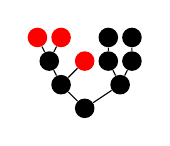
\begin{tikzpicture}[scale=.2]
\node[circle, scale=0.75, fill] (tid0) at (3.75,1.5){};
\node[circle, scale=0.75, fill] (tid1) at (2.25,3){};
\node[circle, scale=0.75, fill] (tid3) at (1.5,4.5){};
\node[circle, scale=0.75, fill, red] (tid7) at (0.75,6){};
\node[circle, scale=0.75, fill, red] (tid8) at (2.25,6){};
\draw[](tid3) -- (tid7);
\draw[](tid3) -- (tid8);
\node[circle, scale=0.75, fill, red] (tid4) at (3.75,4.5){};
\draw[](tid1) -- (tid3);
\draw[](tid1) -- (tid4);
\node[circle, scale=0.75, fill] (tid2) at (6,3){};
\node[circle, scale=0.75, fill] (tid5) at (5.25,4.5){};
\node[circle, scale=0.75, fill] (tid9) at (5.25,6){};
\draw[](tid5) -- (tid9);
\node[circle, scale=0.75, fill] (tid6) at (6.75,4.5){};
\node[circle, scale=0.75, fill] (tid10) at (6.75,6){};
\draw[](tid6) -- (tid10);
\draw[](tid2) -- (tid5);
\draw[](tid2) -- (tid6);
\draw[](tid0) -- (tid1);
\draw[](tid0) -- (tid2);
\end{tikzpicture}
\nodepart{three}
\footnotesize{6.01555}
\nodepart{four}
\footnotesize{$33\:67$}
};
 & 
\node[draw=black, rectangle split,  rectangle split parts=4] (sn0x9b89760){
\footnotesize{22.2222}
\nodepart{two}
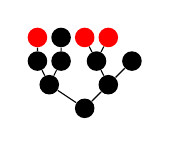
\begin{tikzpicture}[scale=.2]
\node[circle, scale=0.75, fill] (tid0) at (3.75,1.5){};
\node[circle, scale=0.75, fill] (tid1) at (1.5,3){};
\node[circle, scale=0.75, fill] (tid3) at (0.75,4.5){};
\node[circle, scale=0.75, fill, red] (tid7) at (0.75,6){};
\draw[](tid3) -- (tid7);
\node[circle, scale=0.75, fill] (tid4) at (2.25,4.5){};
\node[circle, scale=0.75, fill] (tid8) at (2.25,6){};
\draw[](tid4) -- (tid8);
\draw[](tid1) -- (tid3);
\draw[](tid1) -- (tid4);
\node[circle, scale=0.75, fill] (tid2) at (5.25,3){};
\node[circle, scale=0.75, fill] (tid5) at (4.5,4.5){};
\node[circle, scale=0.75, fill, red] (tid9) at (3.75,6){};
\node[circle, scale=0.75, fill, red] (tid10) at (5.25,6){};
\draw[](tid5) -- (tid9);
\draw[](tid5) -- (tid10);
\node[circle, scale=0.75, fill] (tid6) at (6.75,4.5){};
\draw[](tid2) -- (tid5);
\draw[](tid2) -- (tid6);
\draw[](tid0) -- (tid1);
\draw[](tid0) -- (tid2);
\end{tikzpicture}
\nodepart{three}
\footnotesize{5.97196}
\nodepart{four}
\footnotesize{$33\:11\:11\:11\:33$}
};
 & 
\node[draw=black, rectangle split,  rectangle split parts=4] (sn0x9b89cc0){
\footnotesize{22.2222}
\nodepart{two}
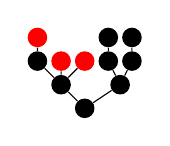
\begin{tikzpicture}[scale=.2]
\node[circle, scale=0.75, fill] (tid0) at (3.75,1.5){};
\node[circle, scale=0.75, fill] (tid1) at (2.25,3){};
\node[circle, scale=0.75, fill] (tid3) at (0.75,4.5){};
\node[circle, scale=0.75, fill, red] (tid8) at (0.75,6){};
\draw[](tid3) -- (tid8);
\node[circle, scale=0.75, fill, red] (tid4) at (2.25,4.5){};
\node[circle, scale=0.75, fill, red] (tid5) at (3.75,4.5){};
\draw[](tid1) -- (tid3);
\draw[](tid1) -- (tid4);
\draw[](tid1) -- (tid5);
\node[circle, scale=0.75, fill] (tid2) at (6,3){};
\node[circle, scale=0.75, fill] (tid6) at (5.25,4.5){};
\node[circle, scale=0.75, fill] (tid9) at (5.25,6){};
\draw[](tid6) -- (tid9);
\node[circle, scale=0.75, fill] (tid7) at (6.75,4.5){};
\node[circle, scale=0.75, fill] (tid10) at (6.75,6){};
\draw[](tid7) -- (tid10);
\draw[](tid2) -- (tid6);
\draw[](tid2) -- (tid7);
\draw[](tid0) -- (tid1);
\draw[](tid0) -- (tid2);
\end{tikzpicture}
\nodepart{three}
\footnotesize{5.97756}
\nodepart{four}
\footnotesize{$67\:11\:22$}
};
 & 
\node[draw=black, rectangle split,  rectangle split parts=4] (sn0x9b8a1f8){
\footnotesize{44.4444}
\nodepart{two}
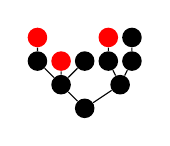
\begin{tikzpicture}[scale=.2]
\node[circle, scale=0.75, fill] (tid0) at (3.75,1.5){};
\node[circle, scale=0.75, fill] (tid1) at (2.25,3){};
\node[circle, scale=0.75, fill] (tid3) at (0.75,4.5){};
\node[circle, scale=0.75, fill, red] (tid8) at (0.75,6){};
\draw[](tid3) -- (tid8);
\node[circle, scale=0.75, fill, red] (tid4) at (2.25,4.5){};
\node[circle, scale=0.75, fill] (tid5) at (3.75,4.5){};
\draw[](tid1) -- (tid3);
\draw[](tid1) -- (tid4);
\draw[](tid1) -- (tid5);
\node[circle, scale=0.75, fill] (tid2) at (6,3){};
\node[circle, scale=0.75, fill] (tid6) at (5.25,4.5){};
\node[circle, scale=0.75, fill, red] (tid9) at (5.25,6){};
\draw[](tid6) -- (tid9);
\node[circle, scale=0.75, fill] (tid7) at (6.75,4.5){};
\node[circle, scale=0.75, fill] (tid10) at (6.75,6){};
\draw[](tid7) -- (tid10);
\draw[](tid2) -- (tid6);
\draw[](tid2) -- (tid7);
\draw[](tid0) -- (tid1);
\draw[](tid0) -- (tid2);
\end{tikzpicture}
\nodepart{three}
\footnotesize{5.93048}
\nodepart{four}
\footnotesize{$17\:17\:22\:11\:11\:11\:11$}
};
 & 
\\
};
\end{scope}
\begin{scope}[yshift=\leveltopIII cm]
\matrix (line3)[column sep=1cm] {
\node[draw=black, rectangle split,  rectangle split parts=4] (sn0x9b8a418){
\footnotesize{3.7037}
\nodepart{two}
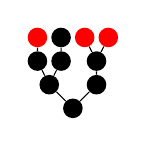
\begin{tikzpicture}[scale=.2]
\node[circle, scale=0.75, fill] (tid0) at (3,1.5){};
\node[circle, scale=0.75, fill] (tid1) at (1.5,3){};
\node[circle, scale=0.75, fill] (tid3) at (0.75,4.5){};
\node[circle, scale=0.75, fill, red] (tid6) at (0.75,6){};
\draw[](tid3) -- (tid6);
\node[circle, scale=0.75, fill] (tid4) at (2.25,4.5){};
\node[circle, scale=0.75, fill] (tid7) at (2.25,6){};
\draw[](tid4) -- (tid7);
\draw[](tid1) -- (tid3);
\draw[](tid1) -- (tid4);
\node[circle, scale=0.75, fill] (tid2) at (4.5,3){};
\node[circle, scale=0.75, fill] (tid5) at (4.5,4.5){};
\node[circle, scale=0.75, fill, red] (tid8) at (3.75,6){};
\node[circle, scale=0.75, fill, red] (tid9) at (5.25,6){};
\draw[](tid5) -- (tid8);
\draw[](tid5) -- (tid9);
\draw[](tid2) -- (tid5);
\draw[](tid0) -- (tid1);
\draw[](tid0) -- (tid2);
\end{tikzpicture}
\nodepart{three}
\footnotesize{5.7278}
\nodepart{four}
\footnotesize{$17\:17\:67$}
};
 & 
\node[draw=black, rectangle split,  rectangle split parts=4] (sn0x9b8aa80){
\footnotesize{37.037}
\nodepart{two}
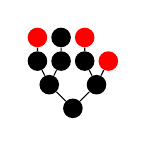
\begin{tikzpicture}[scale=.2]
\node[circle, scale=0.75, fill] (tid0) at (3,1.5){};
\node[circle, scale=0.75, fill] (tid1) at (1.5,3){};
\node[circle, scale=0.75, fill] (tid3) at (0.75,4.5){};
\node[circle, scale=0.75, fill, red] (tid7) at (0.75,6){};
\draw[](tid3) -- (tid7);
\node[circle, scale=0.75, fill] (tid4) at (2.25,4.5){};
\node[circle, scale=0.75, fill] (tid8) at (2.25,6){};
\draw[](tid4) -- (tid8);
\draw[](tid1) -- (tid3);
\draw[](tid1) -- (tid4);
\node[circle, scale=0.75, fill] (tid2) at (4.5,3){};
\node[circle, scale=0.75, fill] (tid5) at (3.75,4.5){};
\node[circle, scale=0.75, fill, red] (tid9) at (3.75,6){};
\draw[](tid5) -- (tid9);
\node[circle, scale=0.75, fill, red] (tid6) at (5.25,4.5){};
\draw[](tid2) -- (tid5);
\draw[](tid2) -- (tid6);
\draw[](tid0) -- (tid1);
\draw[](tid0) -- (tid2);
\end{tikzpicture}
\nodepart{three}
\footnotesize{5.65942}
\nodepart{four}
\footnotesize{$33\:17\:17\:17\:17$}
};
 & 
\node[draw=black, rectangle split,  rectangle split parts=4] (sn0x9b915e0){
\footnotesize{2.46914}
\nodepart{two}
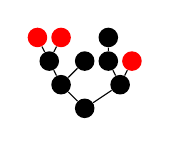
\begin{tikzpicture}[scale=.2]
\node[circle, scale=0.75, fill] (tid0) at (3.75,1.5){};
\node[circle, scale=0.75, fill] (tid1) at (2.25,3){};
\node[circle, scale=0.75, fill] (tid3) at (1.5,4.5){};
\node[circle, scale=0.75, fill, red] (tid7) at (0.75,6){};
\node[circle, scale=0.75, fill, red] (tid8) at (2.25,6){};
\draw[](tid3) -- (tid7);
\draw[](tid3) -- (tid8);
\node[circle, scale=0.75, fill] (tid4) at (3.75,4.5){};
\draw[](tid1) -- (tid3);
\draw[](tid1) -- (tid4);
\node[circle, scale=0.75, fill] (tid2) at (6,3){};
\node[circle, scale=0.75, fill] (tid5) at (5.25,4.5){};
\node[circle, scale=0.75, fill] (tid9) at (5.25,6){};
\draw[](tid5) -- (tid9);
\node[circle, scale=0.75, fill, red] (tid6) at (6.75,4.5){};
\draw[](tid2) -- (tid5);
\draw[](tid2) -- (tid6);
\draw[](tid0) -- (tid1);
\draw[](tid0) -- (tid2);
\end{tikzpicture}
\nodepart{three}
\footnotesize{5.68021}
\nodepart{four}
\footnotesize{$33\:33\:17\:17$}
};
 & 
\node[draw=black, rectangle split,  rectangle split parts=4] (sn0x9b91878){
\footnotesize{2.46914}
\nodepart{two}
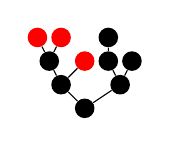
\begin{tikzpicture}[scale=.2]
\node[circle, scale=0.75, fill] (tid0) at (3.75,1.5){};
\node[circle, scale=0.75, fill] (tid1) at (2.25,3){};
\node[circle, scale=0.75, fill] (tid3) at (1.5,4.5){};
\node[circle, scale=0.75, fill, red] (tid7) at (0.75,6){};
\node[circle, scale=0.75, fill, red] (tid8) at (2.25,6){};
\draw[](tid3) -- (tid7);
\draw[](tid3) -- (tid8);
\node[circle, scale=0.75, fill, red] (tid4) at (3.75,4.5){};
\draw[](tid1) -- (tid3);
\draw[](tid1) -- (tid4);
\node[circle, scale=0.75, fill] (tid2) at (6,3){};
\node[circle, scale=0.75, fill] (tid5) at (5.25,4.5){};
\node[circle, scale=0.75, fill] (tid9) at (5.25,6){};
\draw[](tid5) -- (tid9);
\node[circle, scale=0.75, fill] (tid6) at (6.75,4.5){};
\draw[](tid2) -- (tid5);
\draw[](tid2) -- (tid6);
\draw[](tid0) -- (tid1);
\draw[](tid0) -- (tid2);
\end{tikzpicture}
\nodepart{three}
\footnotesize{5.68176}
\nodepart{four}
\footnotesize{$17\:17\:33\:33$}
};
 & 
\node[draw=black, rectangle split,  rectangle split parts=4] (sn0x9b91ba0){
\footnotesize{2.46914}
\nodepart{two}
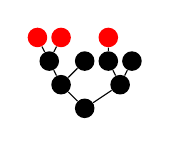
\begin{tikzpicture}[scale=.2]
\node[circle, scale=0.75, fill] (tid0) at (3.75,1.5){};
\node[circle, scale=0.75, fill] (tid1) at (2.25,3){};
\node[circle, scale=0.75, fill] (tid3) at (1.5,4.5){};
\node[circle, scale=0.75, fill, red] (tid7) at (0.75,6){};
\node[circle, scale=0.75, fill, red] (tid8) at (2.25,6){};
\draw[](tid3) -- (tid7);
\draw[](tid3) -- (tid8);
\node[circle, scale=0.75, fill] (tid4) at (3.75,4.5){};
\draw[](tid1) -- (tid3);
\draw[](tid1) -- (tid4);
\node[circle, scale=0.75, fill] (tid2) at (6,3){};
\node[circle, scale=0.75, fill] (tid5) at (5.25,4.5){};
\node[circle, scale=0.75, fill, red] (tid9) at (5.25,6){};
\draw[](tid5) -- (tid9);
\node[circle, scale=0.75, fill] (tid6) at (6.75,4.5){};
\draw[](tid2) -- (tid5);
\draw[](tid2) -- (tid6);
\draw[](tid0) -- (tid1);
\draw[](tid0) -- (tid2);
\end{tikzpicture}
\nodepart{three}
\footnotesize{5.6024}
\nodepart{four}
\footnotesize{$67\:11\:22$}
};
 & 
\node[draw=black, rectangle split,  rectangle split parts=4] (sn0x9b92190){
\footnotesize{14.8148}
\nodepart{two}
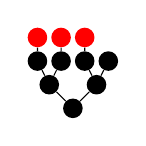
\begin{tikzpicture}[scale=.2]
\node[circle, scale=0.75, fill] (tid0) at (3,1.5){};
\node[circle, scale=0.75, fill] (tid1) at (1.5,3){};
\node[circle, scale=0.75, fill] (tid3) at (0.75,4.5){};
\node[circle, scale=0.75, fill, red] (tid7) at (0.75,6){};
\draw[](tid3) -- (tid7);
\node[circle, scale=0.75, fill] (tid4) at (2.25,4.5){};
\node[circle, scale=0.75, fill, red] (tid8) at (2.25,6){};
\draw[](tid4) -- (tid8);
\draw[](tid1) -- (tid3);
\draw[](tid1) -- (tid4);
\node[circle, scale=0.75, fill] (tid2) at (4.5,3){};
\node[circle, scale=0.75, fill] (tid5) at (3.75,4.5){};
\node[circle, scale=0.75, fill, red] (tid9) at (3.75,6){};
\draw[](tid5) -- (tid9);
\node[circle, scale=0.75, fill] (tid6) at (5.25,4.5){};
\draw[](tid2) -- (tid5);
\draw[](tid2) -- (tid6);
\draw[](tid0) -- (tid1);
\draw[](tid0) -- (tid2);
\end{tikzpicture}
\nodepart{three}
\footnotesize{5.60168}
\nodepart{four}
\footnotesize{$67\:33$}
};
 & 
\node[draw=black, rectangle split,  rectangle split parts=4] (sn0x9b94588){
\footnotesize{2.46914}
\nodepart{two}
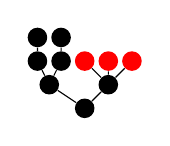
\begin{tikzpicture}[scale=.2]
\node[circle, scale=0.75, fill] (tid0) at (3.75,1.5){};
\node[circle, scale=0.75, fill] (tid1) at (1.5,3){};
\node[circle, scale=0.75, fill] (tid3) at (0.75,4.5){};
\node[circle, scale=0.75, fill] (tid8) at (0.75,6){};
\draw[](tid3) -- (tid8);
\node[circle, scale=0.75, fill] (tid4) at (2.25,4.5){};
\node[circle, scale=0.75, fill] (tid9) at (2.25,6){};
\draw[](tid4) -- (tid9);
\draw[](tid1) -- (tid3);
\draw[](tid1) -- (tid4);
\node[circle, scale=0.75, fill] (tid2) at (5.25,3){};
\node[circle, scale=0.75, fill, red] (tid5) at (3.75,4.5){};
\node[circle, scale=0.75, fill, red] (tid6) at (5.25,4.5){};
\node[circle, scale=0.75, fill, red] (tid7) at (6.75,4.5){};
\draw[](tid2) -- (tid5);
\draw[](tid2) -- (tid6);
\draw[](tid2) -- (tid7);
\draw[](tid0) -- (tid1);
\draw[](tid0) -- (tid2);
\end{tikzpicture}
\nodepart{three}
\footnotesize{5.64738}
\nodepart{four}
\footnotesize{$1$}
};
 & 
\node[draw=black, rectangle split,  rectangle split parts=4] (sn0x9b94698){
\footnotesize{14.8148}
\nodepart{two}
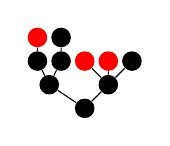
\begin{tikzpicture}[scale=.2]
\node[circle, scale=0.75, fill] (tid0) at (3.75,1.5){};
\node[circle, scale=0.75, fill] (tid1) at (1.5,3){};
\node[circle, scale=0.75, fill] (tid3) at (0.75,4.5){};
\node[circle, scale=0.75, fill, red] (tid8) at (0.75,6){};
\draw[](tid3) -- (tid8);
\node[circle, scale=0.75, fill] (tid4) at (2.25,4.5){};
\node[circle, scale=0.75, fill] (tid9) at (2.25,6){};
\draw[](tid4) -- (tid9);
\draw[](tid1) -- (tid3);
\draw[](tid1) -- (tid4);
\node[circle, scale=0.75, fill] (tid2) at (5.25,3){};
\node[circle, scale=0.75, fill, red] (tid5) at (3.75,4.5){};
\node[circle, scale=0.75, fill, red] (tid6) at (5.25,4.5){};
\node[circle, scale=0.75, fill] (tid7) at (6.75,4.5){};
\draw[](tid2) -- (tid5);
\draw[](tid2) -- (tid6);
\draw[](tid2) -- (tid7);
\draw[](tid0) -- (tid1);
\draw[](tid0) -- (tid2);
\end{tikzpicture}
\nodepart{three}
\footnotesize{5.59704}
\nodepart{four}
\footnotesize{$33\:33\:11\:11\:11$}
};
 & 
\node[draw=black, rectangle split,  rectangle split parts=4] (sn0x9b96f28){
\footnotesize{4.93827}
\nodepart{two}
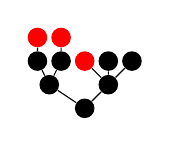
\begin{tikzpicture}[scale=.2]
\node[circle, scale=0.75, fill] (tid0) at (3.75,1.5){};
\node[circle, scale=0.75, fill] (tid1) at (1.5,3){};
\node[circle, scale=0.75, fill] (tid3) at (0.75,4.5){};
\node[circle, scale=0.75, fill, red] (tid8) at (0.75,6){};
\draw[](tid3) -- (tid8);
\node[circle, scale=0.75, fill] (tid4) at (2.25,4.5){};
\node[circle, scale=0.75, fill, red] (tid9) at (2.25,6){};
\draw[](tid4) -- (tid9);
\draw[](tid1) -- (tid3);
\draw[](tid1) -- (tid4);
\node[circle, scale=0.75, fill] (tid2) at (5.25,3){};
\node[circle, scale=0.75, fill, red] (tid5) at (3.75,4.5){};
\node[circle, scale=0.75, fill] (tid6) at (5.25,4.5){};
\node[circle, scale=0.75, fill] (tid7) at (6.75,4.5){};
\draw[](tid2) -- (tid5);
\draw[](tid2) -- (tid6);
\draw[](tid2) -- (tid7);
\draw[](tid0) -- (tid1);
\draw[](tid0) -- (tid2);
\end{tikzpicture}
\nodepart{three}
\footnotesize{5.52543}
\nodepart{four}
\footnotesize{$33\:44\:22$}
};
 & 
\node[draw=black, rectangle split,  rectangle split parts=4] (sn0x9b97408){
\footnotesize{4.93827}
\nodepart{two}
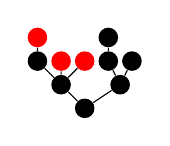
\begin{tikzpicture}[scale=.2]
\node[circle, scale=0.75, fill] (tid0) at (3.75,1.5){};
\node[circle, scale=0.75, fill] (tid1) at (2.25,3){};
\node[circle, scale=0.75, fill] (tid3) at (0.75,4.5){};
\node[circle, scale=0.75, fill, red] (tid8) at (0.75,6){};
\draw[](tid3) -- (tid8);
\node[circle, scale=0.75, fill, red] (tid4) at (2.25,4.5){};
\node[circle, scale=0.75, fill, red] (tid5) at (3.75,4.5){};
\draw[](tid1) -- (tid3);
\draw[](tid1) -- (tid4);
\draw[](tid1) -- (tid5);
\node[circle, scale=0.75, fill] (tid2) at (6,3){};
\node[circle, scale=0.75, fill] (tid6) at (5.25,4.5){};
\node[circle, scale=0.75, fill] (tid9) at (5.25,6){};
\draw[](tid6) -- (tid9);
\node[circle, scale=0.75, fill] (tid7) at (6.75,4.5){};
\draw[](tid2) -- (tid6);
\draw[](tid2) -- (tid7);
\draw[](tid0) -- (tid1);
\draw[](tid0) -- (tid2);
\end{tikzpicture}
\nodepart{three}
\footnotesize{5.61513}
\nodepart{four}
\footnotesize{$33\:33\:11\:11\:11$}
};
 & 
\node[draw=black, rectangle split,  rectangle split parts=4] (sn0x9b97470){
\footnotesize{4.93827}
\nodepart{two}
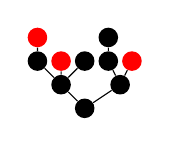
\begin{tikzpicture}[scale=.2]
\node[circle, scale=0.75, fill] (tid0) at (3.75,1.5){};
\node[circle, scale=0.75, fill] (tid1) at (2.25,3){};
\node[circle, scale=0.75, fill] (tid3) at (0.75,4.5){};
\node[circle, scale=0.75, fill, red] (tid8) at (0.75,6){};
\draw[](tid3) -- (tid8);
\node[circle, scale=0.75, fill, red] (tid4) at (2.25,4.5){};
\node[circle, scale=0.75, fill] (tid5) at (3.75,4.5){};
\draw[](tid1) -- (tid3);
\draw[](tid1) -- (tid4);
\draw[](tid1) -- (tid5);
\node[circle, scale=0.75, fill] (tid2) at (6,3){};
\node[circle, scale=0.75, fill] (tid6) at (5.25,4.5){};
\node[circle, scale=0.75, fill] (tid9) at (5.25,6){};
\draw[](tid6) -- (tid9);
\node[circle, scale=0.75, fill, red] (tid7) at (6.75,4.5){};
\draw[](tid2) -- (tid6);
\draw[](tid2) -- (tid7);
\draw[](tid0) -- (tid1);
\draw[](tid0) -- (tid2);
\end{tikzpicture}
\nodepart{three}
\footnotesize{5.61751}
\nodepart{four}
\footnotesize{$17\:17\:22\:11\:17\:17$}
};
 & 
\node[draw=black, rectangle split,  rectangle split parts=4] (sn0x9b97d88){
\footnotesize{4.93827}
\nodepart{two}
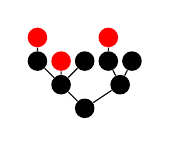
\begin{tikzpicture}[scale=.2]
\node[circle, scale=0.75, fill] (tid0) at (3.75,1.5){};
\node[circle, scale=0.75, fill] (tid1) at (2.25,3){};
\node[circle, scale=0.75, fill] (tid3) at (0.75,4.5){};
\node[circle, scale=0.75, fill, red] (tid8) at (0.75,6){};
\draw[](tid3) -- (tid8);
\node[circle, scale=0.75, fill, red] (tid4) at (2.25,4.5){};
\node[circle, scale=0.75, fill] (tid5) at (3.75,4.5){};
\draw[](tid1) -- (tid3);
\draw[](tid1) -- (tid4);
\draw[](tid1) -- (tid5);
\node[circle, scale=0.75, fill] (tid2) at (6,3){};
\node[circle, scale=0.75, fill] (tid6) at (5.25,4.5){};
\node[circle, scale=0.75, fill, red] (tid9) at (5.25,6){};
\draw[](tid6) -- (tid9);
\node[circle, scale=0.75, fill] (tid7) at (6.75,4.5){};
\draw[](tid2) -- (tid6);
\draw[](tid2) -- (tid7);
\draw[](tid0) -- (tid1);
\draw[](tid0) -- (tid2);
\end{tikzpicture}
\nodepart{three}
\footnotesize{5.53048}
\nodepart{four}
\footnotesize{$33\:22\:11\:11\:22$}
};
 & 
\\
};
\end{scope}
\draw (sn0x9b86e80.south) -- (sn0x9b89f18.north);
\draw (sn0x9b86e80.south) -- (sn0x9b89760.north);
\draw (sn0x9b86e80.south) -- (sn0x9b89cc0.north);
\draw (sn0x9b86e80.south) -- (sn0x9b8a1f8.north);
\draw (sn0x9b89f18.south) -- (sn0x9b8a418.north);
\draw (sn0x9b89f18.south) -- (sn0x9b8aa80.north);
\draw (sn0x9b89760.south) -- (sn0x9b915e0.north);
\draw (sn0x9b89760.south) -- (sn0x9b91878.north);
\draw (sn0x9b89760.south) -- (sn0x9b91ba0.north);
\draw (sn0x9b89760.south) -- (sn0x9b8aa80.north);
\draw (sn0x9b89760.south) -- (sn0x9b92190.north);
\draw (sn0x9b89cc0.south) -- (sn0x9b8aa80.north);
\draw (sn0x9b89cc0.south) -- (sn0x9b94588.north);
\draw (sn0x9b89cc0.south) -- (sn0x9b94698.north);
\draw (sn0x9b8a1f8.south) -- (sn0x9b8aa80.north);
\draw (sn0x9b8a1f8.south) -- (sn0x9b92190.north);
\draw (sn0x9b8a1f8.south) -- (sn0x9b94698.north);
\draw (sn0x9b8a1f8.south) -- (sn0x9b96f28.north);
\draw (sn0x9b8a1f8.south) -- (sn0x9b97408.north);
\draw (sn0x9b8a1f8.south) -- (sn0x9b97470.north);
\draw (sn0x9b8a1f8.south) -- (sn0x9b97d88.north);
\end{tikzpicture}

%%% Local Variables:
%%% TeX-master: "thesis/thesis.tex"
%%% End: 
\renewcommand{\leveltopI}{-15cm + \leveltop}
\renewcommand{\leveltopII}{-15cm + \leveltopI}
\renewcommand{\leveltopIII}{-15cm + \leveltopII}
\renewcommand{\leveltopIIII}{-15cm + \leveltopIII}
\renewcommand{\leveltopIIIII}{-15cm + \leveltopIIII}
\renewcommand{\leveltopIIIIII}{-15cm + \leveltopIIIII}
\renewcommand{\leveltopIIIIIII}{-15cm + \leveltopIIIIII}
\renewcommand{\leveltopIIIIIIII}{-15cm + \leveltopIIIIIII}
\renewcommand{\leveltopIIIIIIIII}{-15cm + \leveltopIIIIIIII}
\renewcommand{\leveltopIIIIIIIIII}{-15cm + \leveltopIIIIIIIII}
\renewcommand{\leveltopIIIIIIIIIII}{-15cm + \leveltopIIIIIIIIII}
\renewcommand{\leveltopIIIIIIIIIIII}{-15cm + \leveltopIIIIIIIIIII}
\begin{tikzpicture}[scale=.2, anchor=south]
\begin{scope}[yshift=\leveltopI cm]
\matrix (line1)[column sep=1cm] {
\node[draw=black, rectangle split,  rectangle split parts=4] (sn0x9b87328){
\footnotesize{100}
\nodepart{two}
\begin{tikzpicture}[scale=.2]
\node[circle, scale=0.75, fill] (tid0) at (4.5,1.5){};
\node[circle, scale=0.75, fill] (tid1) at (3,3){};
\node[circle, scale=0.75, fill] (tid3) at (1.5,4.5){};
\node[circle, scale=0.75, fill] (tid8) at (0.75,6){};
\node[circle, scale=0.75, fill] (tid9) at (2.25,6){};
\draw[](tid3) -- (tid8);
\draw[](tid3) -- (tid9);
\node[circle, scale=0.75, fill, red] (tid4) at (3.75,4.5){};
\node[circle, scale=0.75, fill, red] (tid5) at (5.25,4.5){};
\draw[](tid1) -- (tid3);
\draw[](tid1) -- (tid4);
\draw[](tid1) -- (tid5);
\node[circle, scale=0.75, fill] (tid2) at (7.5,3){};
\node[circle, scale=0.75, fill] (tid6) at (6.75,4.5){};
\node[circle, scale=0.75, fill, red] (tid10) at (6.75,6){};
\draw[](tid6) -- (tid10);
\node[circle, scale=0.75, fill] (tid7) at (8.25,4.5){};
\node[circle, scale=0.75, fill] (tid11) at (8.25,6){};
\draw[](tid7) -- (tid11);
\draw[](tid2) -- (tid6);
\draw[](tid2) -- (tid7);
\draw[](tid0) -- (tid1);
\draw[](tid0) -- (tid2);
\end{tikzpicture}
\nodepart{three}
\footnotesize{6.3725}
\nodepart{four}
\footnotesize{$44\:22\:8.3\:17\:8.3$}
};
 & 
\\
};
\end{scope}
\begin{scope}[yshift=\leveltopII cm]
\matrix (line2)[column sep=1cm] {
\node[draw=black, rectangle split,  rectangle split parts=4] (sn0x9b9a400){
\footnotesize{44.4444}
\nodepart{two}
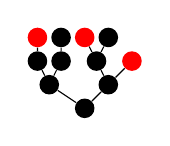
\begin{tikzpicture}[scale=.2]
\node[circle, scale=0.75, fill] (tid0) at (3.75,1.5){};
\node[circle, scale=0.75, fill] (tid1) at (1.5,3){};
\node[circle, scale=0.75, fill] (tid3) at (0.75,4.5){};
\node[circle, scale=0.75, fill, red] (tid7) at (0.75,6){};
\draw[](tid3) -- (tid7);
\node[circle, scale=0.75, fill] (tid4) at (2.25,4.5){};
\node[circle, scale=0.75, fill] (tid8) at (2.25,6){};
\draw[](tid4) -- (tid8);
\draw[](tid1) -- (tid3);
\draw[](tid1) -- (tid4);
\node[circle, scale=0.75, fill] (tid2) at (5.25,3){};
\node[circle, scale=0.75, fill] (tid5) at (4.5,4.5){};
\node[circle, scale=0.75, fill, red] (tid9) at (3.75,6){};
\node[circle, scale=0.75, fill] (tid10) at (5.25,6){};
\draw[](tid5) -- (tid9);
\draw[](tid5) -- (tid10);
\node[circle, scale=0.75, fill, red] (tid6) at (6.75,4.5){};
\draw[](tid2) -- (tid5);
\draw[](tid2) -- (tid6);
\draw[](tid0) -- (tid1);
\draw[](tid0) -- (tid2);
\end{tikzpicture}
\nodepart{three}
\footnotesize{6.03469}
\nodepart{four}
\footnotesize{$17\:17\:11\:11\:11\:17\:17$}
};
 & 
\node[draw=black, rectangle split,  rectangle split parts=4] (sn0x9b9aab0){
\footnotesize{22.2222}
\nodepart{two}
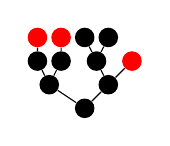
\begin{tikzpicture}[scale=.2]
\node[circle, scale=0.75, fill] (tid0) at (3.75,1.5){};
\node[circle, scale=0.75, fill] (tid1) at (1.5,3){};
\node[circle, scale=0.75, fill] (tid3) at (0.75,4.5){};
\node[circle, scale=0.75, fill, red] (tid7) at (0.75,6){};
\draw[](tid3) -- (tid7);
\node[circle, scale=0.75, fill] (tid4) at (2.25,4.5){};
\node[circle, scale=0.75, fill, red] (tid8) at (2.25,6){};
\draw[](tid4) -- (tid8);
\draw[](tid1) -- (tid3);
\draw[](tid1) -- (tid4);
\node[circle, scale=0.75, fill] (tid2) at (5.25,3){};
\node[circle, scale=0.75, fill] (tid5) at (4.5,4.5){};
\node[circle, scale=0.75, fill] (tid9) at (3.75,6){};
\node[circle, scale=0.75, fill] (tid10) at (5.25,6){};
\draw[](tid5) -- (tid9);
\draw[](tid5) -- (tid10);
\node[circle, scale=0.75, fill, red] (tid6) at (6.75,4.5){};
\draw[](tid2) -- (tid5);
\draw[](tid2) -- (tid6);
\draw[](tid0) -- (tid1);
\draw[](tid0) -- (tid2);
\end{tikzpicture}
\nodepart{three}
\footnotesize{6.05253}
\nodepart{four}
\footnotesize{$33\:44\:22$}
};
 & 
\node[draw=black, rectangle split,  rectangle split parts=4] (sn0x9b9ab88){
\footnotesize{8.33333}
\nodepart{two}
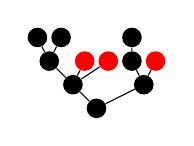
\begin{tikzpicture}[scale=.2]
\node[circle, scale=0.75, fill] (tid0) at (4.5,1.5){};
\node[circle, scale=0.75, fill] (tid1) at (3,3){};
\node[circle, scale=0.75, fill] (tid3) at (1.5,4.5){};
\node[circle, scale=0.75, fill] (tid8) at (0.75,6){};
\node[circle, scale=0.75, fill] (tid9) at (2.25,6){};
\draw[](tid3) -- (tid8);
\draw[](tid3) -- (tid9);
\node[circle, scale=0.75, fill, red] (tid4) at (3.75,4.5){};
\node[circle, scale=0.75, fill, red] (tid5) at (5.25,4.5){};
\draw[](tid1) -- (tid3);
\draw[](tid1) -- (tid4);
\draw[](tid1) -- (tid5);
\node[circle, scale=0.75, fill] (tid2) at (7.5,3){};
\node[circle, scale=0.75, fill] (tid6) at (6.75,4.5){};
\node[circle, scale=0.75, fill] (tid10) at (6.75,6){};
\draw[](tid6) -- (tid10);
\node[circle, scale=0.75, fill, red] (tid7) at (8.25,4.5){};
\draw[](tid2) -- (tid6);
\draw[](tid2) -- (tid7);
\draw[](tid0) -- (tid1);
\draw[](tid0) -- (tid2);
\end{tikzpicture}
\nodepart{three}
\footnotesize{6.08635}
\nodepart{four}
\footnotesize{$44\:22\:22\:11$}
};
 & 
\node[draw=black, rectangle split,  rectangle split parts=4] (sn0x9b9a468){
\footnotesize{16.6667}
\nodepart{two}
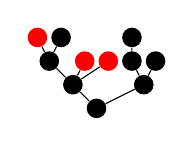
\begin{tikzpicture}[scale=.2]
\node[circle, scale=0.75, fill] (tid0) at (4.5,1.5){};
\node[circle, scale=0.75, fill] (tid1) at (3,3){};
\node[circle, scale=0.75, fill] (tid3) at (1.5,4.5){};
\node[circle, scale=0.75, fill, red] (tid8) at (0.75,6){};
\node[circle, scale=0.75, fill] (tid9) at (2.25,6){};
\draw[](tid3) -- (tid8);
\draw[](tid3) -- (tid9);
\node[circle, scale=0.75, fill, red] (tid4) at (3.75,4.5){};
\node[circle, scale=0.75, fill, red] (tid5) at (5.25,4.5){};
\draw[](tid1) -- (tid3);
\draw[](tid1) -- (tid4);
\draw[](tid1) -- (tid5);
\node[circle, scale=0.75, fill] (tid2) at (7.5,3){};
\node[circle, scale=0.75, fill] (tid6) at (6.75,4.5){};
\node[circle, scale=0.75, fill] (tid10) at (6.75,6){};
\draw[](tid6) -- (tid10);
\node[circle, scale=0.75, fill] (tid7) at (8.25,4.5){};
\draw[](tid2) -- (tid6);
\draw[](tid2) -- (tid7);
\draw[](tid0) -- (tid1);
\draw[](tid0) -- (tid2);
\end{tikzpicture}
\nodepart{three}
\footnotesize{6.01642}
\nodepart{four}
\footnotesize{$22\:22\:22\:11\:11\:11$}
};
 & 
\node[draw=black, rectangle split,  rectangle split parts=4] (sn0x9b9b1b8){
\footnotesize{8.33333}
\nodepart{two}
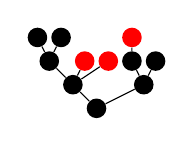
\begin{tikzpicture}[scale=.2]
\node[circle, scale=0.75, fill] (tid0) at (4.5,1.5){};
\node[circle, scale=0.75, fill] (tid1) at (3,3){};
\node[circle, scale=0.75, fill] (tid3) at (1.5,4.5){};
\node[circle, scale=0.75, fill] (tid8) at (0.75,6){};
\node[circle, scale=0.75, fill] (tid9) at (2.25,6){};
\draw[](tid3) -- (tid8);
\draw[](tid3) -- (tid9);
\node[circle, scale=0.75, fill, red] (tid4) at (3.75,4.5){};
\node[circle, scale=0.75, fill, red] (tid5) at (5.25,4.5){};
\draw[](tid1) -- (tid3);
\draw[](tid1) -- (tid4);
\draw[](tid1) -- (tid5);
\node[circle, scale=0.75, fill] (tid2) at (7.5,3){};
\node[circle, scale=0.75, fill] (tid6) at (6.75,4.5){};
\node[circle, scale=0.75, fill, red] (tid10) at (6.75,6){};
\draw[](tid6) -- (tid10);
\node[circle, scale=0.75, fill] (tid7) at (8.25,4.5){};
\draw[](tid2) -- (tid6);
\draw[](tid2) -- (tid7);
\draw[](tid0) -- (tid1);
\draw[](tid0) -- (tid2);
\end{tikzpicture}
\nodepart{three}
\footnotesize{6.02577}
\nodepart{four}
\footnotesize{$44\:22\:17\:17$}
};
 & 
\\
};
\end{scope}
\begin{scope}[yshift=\leveltopIII cm]
\matrix (line3)[column sep=1cm] {
\node[draw=black, rectangle split,  rectangle split parts=4] (sn0x9b9bcf0){
\footnotesize{14.8148}
\nodepart{two}
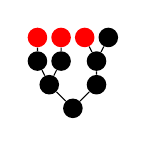
\begin{tikzpicture}[scale=.2]
\node[circle, scale=0.75, fill] (tid0) at (3,1.5){};
\node[circle, scale=0.75, fill] (tid1) at (1.5,3){};
\node[circle, scale=0.75, fill] (tid3) at (0.75,4.5){};
\node[circle, scale=0.75, fill, red] (tid6) at (0.75,6){};
\draw[](tid3) -- (tid6);
\node[circle, scale=0.75, fill] (tid4) at (2.25,4.5){};
\node[circle, scale=0.75, fill, red] (tid7) at (2.25,6){};
\draw[](tid4) -- (tid7);
\draw[](tid1) -- (tid3);
\draw[](tid1) -- (tid4);
\node[circle, scale=0.75, fill] (tid2) at (4.5,3){};
\node[circle, scale=0.75, fill] (tid5) at (4.5,4.5){};
\node[circle, scale=0.75, fill, red] (tid8) at (3.75,6){};
\node[circle, scale=0.75, fill] (tid9) at (5.25,6){};
\draw[](tid5) -- (tid8);
\draw[](tid5) -- (tid9);
\draw[](tid2) -- (tid5);
\draw[](tid0) -- (tid1);
\draw[](tid0) -- (tid2);
\end{tikzpicture}
\nodepart{three}
\footnotesize{5.74108}
\nodepart{four}
\footnotesize{$33\:33\:33$}
};
 & 
\node[draw=black, rectangle split,  rectangle split parts=4] (sn0x9b8a418){
\footnotesize{7.40741}
\nodepart{two}
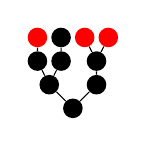
\begin{tikzpicture}[scale=.2]
\node[circle, scale=0.75, fill] (tid0) at (3,1.5){};
\node[circle, scale=0.75, fill] (tid1) at (1.5,3){};
\node[circle, scale=0.75, fill] (tid3) at (0.75,4.5){};
\node[circle, scale=0.75, fill, red] (tid6) at (0.75,6){};
\draw[](tid3) -- (tid6);
\node[circle, scale=0.75, fill] (tid4) at (2.25,4.5){};
\node[circle, scale=0.75, fill] (tid7) at (2.25,6){};
\draw[](tid4) -- (tid7);
\draw[](tid1) -- (tid3);
\draw[](tid1) -- (tid4);
\node[circle, scale=0.75, fill] (tid2) at (4.5,3){};
\node[circle, scale=0.75, fill] (tid5) at (4.5,4.5){};
\node[circle, scale=0.75, fill, red] (tid8) at (3.75,6){};
\node[circle, scale=0.75, fill, red] (tid9) at (5.25,6){};
\draw[](tid5) -- (tid8);
\draw[](tid5) -- (tid9);
\draw[](tid2) -- (tid5);
\draw[](tid0) -- (tid1);
\draw[](tid0) -- (tid2);
\end{tikzpicture}
\nodepart{three}
\footnotesize{5.7278}
\nodepart{four}
\footnotesize{$17\:67\:17$}
};
 & 
\node[draw=black, rectangle split,  rectangle split parts=4] (sn0x9b9bb78){
\footnotesize{12.3457}
\nodepart{two}
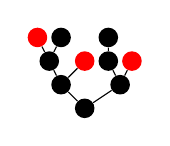
\begin{tikzpicture}[scale=.2]
\node[circle, scale=0.75, fill] (tid0) at (3.75,1.5){};
\node[circle, scale=0.75, fill] (tid1) at (2.25,3){};
\node[circle, scale=0.75, fill] (tid3) at (1.5,4.5){};
\node[circle, scale=0.75, fill, red] (tid7) at (0.75,6){};
\node[circle, scale=0.75, fill] (tid8) at (2.25,6){};
\draw[](tid3) -- (tid7);
\draw[](tid3) -- (tid8);
\node[circle, scale=0.75, fill, red] (tid4) at (3.75,4.5){};
\draw[](tid1) -- (tid3);
\draw[](tid1) -- (tid4);
\node[circle, scale=0.75, fill] (tid2) at (6,3){};
\node[circle, scale=0.75, fill] (tid5) at (5.25,4.5){};
\node[circle, scale=0.75, fill] (tid9) at (5.25,6){};
\draw[](tid5) -- (tid9);
\node[circle, scale=0.75, fill, red] (tid6) at (6.75,4.5){};
\draw[](tid2) -- (tid5);
\draw[](tid2) -- (tid6);
\draw[](tid0) -- (tid1);
\draw[](tid0) -- (tid2);
\end{tikzpicture}
\nodepart{three}
\footnotesize{5.75146}
\nodepart{four}
\footnotesize{$17\:17\:17\:17\:33$}
};
 & 
\node[draw=black, rectangle split,  rectangle split parts=4] (sn0x9b9c080){
\footnotesize{22.2222}
\nodepart{two}
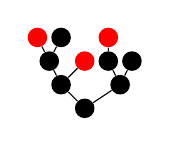
\begin{tikzpicture}[scale=.2]
\node[circle, scale=0.75, fill] (tid0) at (3.75,1.5){};
\node[circle, scale=0.75, fill] (tid1) at (2.25,3){};
\node[circle, scale=0.75, fill] (tid3) at (1.5,4.5){};
\node[circle, scale=0.75, fill, red] (tid7) at (0.75,6){};
\node[circle, scale=0.75, fill] (tid8) at (2.25,6){};
\draw[](tid3) -- (tid7);
\draw[](tid3) -- (tid8);
\node[circle, scale=0.75, fill, red] (tid4) at (3.75,4.5){};
\draw[](tid1) -- (tid3);
\draw[](tid1) -- (tid4);
\node[circle, scale=0.75, fill] (tid2) at (6,3){};
\node[circle, scale=0.75, fill] (tid5) at (5.25,4.5){};
\node[circle, scale=0.75, fill, red] (tid9) at (5.25,6){};
\draw[](tid5) -- (tid9);
\node[circle, scale=0.75, fill] (tid6) at (6.75,4.5){};
\draw[](tid2) -- (tid5);
\draw[](tid2) -- (tid6);
\draw[](tid0) -- (tid1);
\draw[](tid0) -- (tid2);
\end{tikzpicture}
\nodepart{three}
\footnotesize{5.68383}
\nodepart{four}
\footnotesize{$17\:17\:17\:17\:22\:11$}
};
 & 
\node[draw=black, rectangle split,  rectangle split parts=4] (sn0x9b91878){
\footnotesize{8.64198}
\nodepart{two}
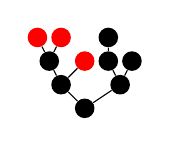
\begin{tikzpicture}[scale=.2]
\node[circle, scale=0.75, fill] (tid0) at (3.75,1.5){};
\node[circle, scale=0.75, fill] (tid1) at (2.25,3){};
\node[circle, scale=0.75, fill] (tid3) at (1.5,4.5){};
\node[circle, scale=0.75, fill, red] (tid7) at (0.75,6){};
\node[circle, scale=0.75, fill, red] (tid8) at (2.25,6){};
\draw[](tid3) -- (tid7);
\draw[](tid3) -- (tid8);
\node[circle, scale=0.75, fill, red] (tid4) at (3.75,4.5){};
\draw[](tid1) -- (tid3);
\draw[](tid1) -- (tid4);
\node[circle, scale=0.75, fill] (tid2) at (6,3){};
\node[circle, scale=0.75, fill] (tid5) at (5.25,4.5){};
\node[circle, scale=0.75, fill] (tid9) at (5.25,6){};
\draw[](tid5) -- (tid9);
\node[circle, scale=0.75, fill] (tid6) at (6.75,4.5){};
\draw[](tid2) -- (tid5);
\draw[](tid2) -- (tid6);
\draw[](tid0) -- (tid1);
\draw[](tid0) -- (tid2);
\end{tikzpicture}
\nodepart{three}
\footnotesize{5.68176}
\nodepart{four}
\footnotesize{$17\:17\:33\:33$}
};
 & 
\node[draw=black, rectangle split,  rectangle split parts=4] (sn0x9b9c560){
\footnotesize{7.40741}
\nodepart{two}
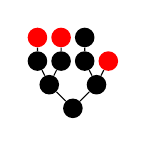
\begin{tikzpicture}[scale=.2]
\node[circle, scale=0.75, fill] (tid0) at (3,1.5){};
\node[circle, scale=0.75, fill] (tid1) at (1.5,3){};
\node[circle, scale=0.75, fill] (tid3) at (0.75,4.5){};
\node[circle, scale=0.75, fill, red] (tid7) at (0.75,6){};
\draw[](tid3) -- (tid7);
\node[circle, scale=0.75, fill] (tid4) at (2.25,4.5){};
\node[circle, scale=0.75, fill, red] (tid8) at (2.25,6){};
\draw[](tid4) -- (tid8);
\draw[](tid1) -- (tid3);
\draw[](tid1) -- (tid4);
\node[circle, scale=0.75, fill] (tid2) at (4.5,3){};
\node[circle, scale=0.75, fill] (tid5) at (3.75,4.5){};
\node[circle, scale=0.75, fill] (tid9) at (3.75,6){};
\draw[](tid5) -- (tid9);
\node[circle, scale=0.75, fill, red] (tid6) at (5.25,4.5){};
\draw[](tid2) -- (tid5);
\draw[](tid2) -- (tid6);
\draw[](tid0) -- (tid1);
\draw[](tid0) -- (tid2);
\end{tikzpicture}
\nodepart{three}
\footnotesize{5.66847}
\nodepart{four}
\footnotesize{$33\:33\:33$}
};
 & 
\node[draw=black, rectangle split,  rectangle split parts=4] (sn0x9b8aa80){
\footnotesize{7.40741}
\nodepart{two}
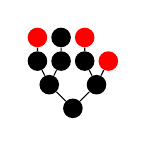
\begin{tikzpicture}[scale=.2]
\node[circle, scale=0.75, fill] (tid0) at (3,1.5){};
\node[circle, scale=0.75, fill] (tid1) at (1.5,3){};
\node[circle, scale=0.75, fill] (tid3) at (0.75,4.5){};
\node[circle, scale=0.75, fill, red] (tid7) at (0.75,6){};
\draw[](tid3) -- (tid7);
\node[circle, scale=0.75, fill] (tid4) at (2.25,4.5){};
\node[circle, scale=0.75, fill] (tid8) at (2.25,6){};
\draw[](tid4) -- (tid8);
\draw[](tid1) -- (tid3);
\draw[](tid1) -- (tid4);
\node[circle, scale=0.75, fill] (tid2) at (4.5,3){};
\node[circle, scale=0.75, fill] (tid5) at (3.75,4.5){};
\node[circle, scale=0.75, fill, red] (tid9) at (3.75,6){};
\draw[](tid5) -- (tid9);
\node[circle, scale=0.75, fill, red] (tid6) at (5.25,4.5){};
\draw[](tid2) -- (tid5);
\draw[](tid2) -- (tid6);
\draw[](tid0) -- (tid1);
\draw[](tid0) -- (tid2);
\end{tikzpicture}
\nodepart{three}
\footnotesize{5.65942}
\nodepart{four}
\footnotesize{$33\:17\:17\:17\:17$}
};
 & 
\node[draw=black, rectangle split,  rectangle split parts=4] (sn0x9b9dd18){
\footnotesize{8.64198}
\nodepart{two}
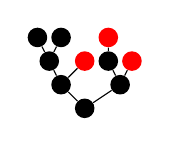
\begin{tikzpicture}[scale=.2]
\node[circle, scale=0.75, fill] (tid0) at (3.75,1.5){};
\node[circle, scale=0.75, fill] (tid1) at (2.25,3){};
\node[circle, scale=0.75, fill] (tid3) at (1.5,4.5){};
\node[circle, scale=0.75, fill] (tid7) at (0.75,6){};
\node[circle, scale=0.75, fill] (tid8) at (2.25,6){};
\draw[](tid3) -- (tid7);
\draw[](tid3) -- (tid8);
\node[circle, scale=0.75, fill, red] (tid4) at (3.75,4.5){};
\draw[](tid1) -- (tid3);
\draw[](tid1) -- (tid4);
\node[circle, scale=0.75, fill] (tid2) at (6,3){};
\node[circle, scale=0.75, fill] (tid5) at (5.25,4.5){};
\node[circle, scale=0.75, fill, red] (tid9) at (5.25,6){};
\draw[](tid5) -- (tid9);
\node[circle, scale=0.75, fill, red] (tid6) at (6.75,4.5){};
\draw[](tid2) -- (tid5);
\draw[](tid2) -- (tid6);
\draw[](tid0) -- (tid1);
\draw[](tid0) -- (tid2);
\end{tikzpicture}
\nodepart{three}
\footnotesize{5.75709}
\nodepart{four}
\footnotesize{$33\:33\:22\:11$}
};
 & 
\node[draw=black, rectangle split,  rectangle split parts=4] (sn0x9b9e468){
\footnotesize{1.85185}
\nodepart{two}
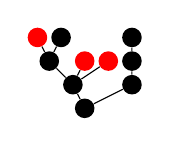
\begin{tikzpicture}[scale=.2]
\node[circle, scale=0.75, fill] (tid0) at (3.75,1.5){};
\node[circle, scale=0.75, fill] (tid1) at (3,3){};
\node[circle, scale=0.75, fill] (tid3) at (1.5,4.5){};
\node[circle, scale=0.75, fill, red] (tid7) at (0.75,6){};
\node[circle, scale=0.75, fill] (tid8) at (2.25,6){};
\draw[](tid3) -- (tid7);
\draw[](tid3) -- (tid8);
\node[circle, scale=0.75, fill, red] (tid4) at (3.75,4.5){};
\node[circle, scale=0.75, fill, red] (tid5) at (5.25,4.5){};
\draw[](tid1) -- (tid3);
\draw[](tid1) -- (tid4);
\draw[](tid1) -- (tid5);
\node[circle, scale=0.75, fill] (tid2) at (6.75,3){};
\node[circle, scale=0.75, fill] (tid6) at (6.75,4.5){};
\node[circle, scale=0.75, fill] (tid9) at (6.75,6){};
\draw[](tid6) -- (tid9);
\draw[](tid2) -- (tid6);
\draw[](tid0) -- (tid1);
\draw[](tid0) -- (tid2);
\end{tikzpicture}
\nodepart{three}
\footnotesize{5.75103}
\nodepart{four}
\footnotesize{$33\:33\:17\:17$}
};
 & 
\node[draw=black, rectangle split,  rectangle split parts=4] (sn0x9b9db98){
\footnotesize{0.925926}
\nodepart{two}
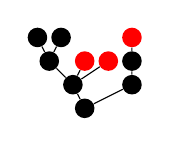
\begin{tikzpicture}[scale=.2]
\node[circle, scale=0.75, fill] (tid0) at (3.75,1.5){};
\node[circle, scale=0.75, fill] (tid1) at (3,3){};
\node[circle, scale=0.75, fill] (tid3) at (1.5,4.5){};
\node[circle, scale=0.75, fill] (tid7) at (0.75,6){};
\node[circle, scale=0.75, fill] (tid8) at (2.25,6){};
\draw[](tid3) -- (tid7);
\draw[](tid3) -- (tid8);
\node[circle, scale=0.75, fill, red] (tid4) at (3.75,4.5){};
\node[circle, scale=0.75, fill, red] (tid5) at (5.25,4.5){};
\draw[](tid1) -- (tid3);
\draw[](tid1) -- (tid4);
\draw[](tid1) -- (tid5);
\node[circle, scale=0.75, fill] (tid2) at (6.75,3){};
\node[circle, scale=0.75, fill] (tid6) at (6.75,4.5){};
\node[circle, scale=0.75, fill, red] (tid9) at (6.75,6){};
\draw[](tid6) -- (tid9);
\draw[](tid2) -- (tid6);
\draw[](tid0) -- (tid1);
\draw[](tid0) -- (tid2);
\end{tikzpicture}
\nodepart{three}
\footnotesize{5.75509}
\nodepart{four}
\footnotesize{$67\:11\:22$}
};
 & 
\node[draw=black, rectangle split,  rectangle split parts=4] (sn0x9ba10a0){
\footnotesize{1.85185}
\nodepart{two}
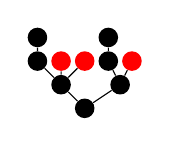
\begin{tikzpicture}[scale=.2]
\node[circle, scale=0.75, fill] (tid0) at (3.75,1.5){};
\node[circle, scale=0.75, fill] (tid1) at (2.25,3){};
\node[circle, scale=0.75, fill] (tid3) at (0.75,4.5){};
\node[circle, scale=0.75, fill] (tid8) at (0.75,6){};
\draw[](tid3) -- (tid8);
\node[circle, scale=0.75, fill, red] (tid4) at (2.25,4.5){};
\node[circle, scale=0.75, fill, red] (tid5) at (3.75,4.5){};
\draw[](tid1) -- (tid3);
\draw[](tid1) -- (tid4);
\draw[](tid1) -- (tid5);
\node[circle, scale=0.75, fill] (tid2) at (6,3){};
\node[circle, scale=0.75, fill] (tid6) at (5.25,4.5){};
\node[circle, scale=0.75, fill] (tid9) at (5.25,6){};
\draw[](tid6) -- (tid9);
\node[circle, scale=0.75, fill, red] (tid7) at (6.75,4.5){};
\draw[](tid2) -- (tid6);
\draw[](tid2) -- (tid7);
\draw[](tid0) -- (tid1);
\draw[](tid0) -- (tid2);
\end{tikzpicture}
\nodepart{three}
\footnotesize{5.68347}
\nodepart{four}
\footnotesize{$67\:17\:17$}
};
 & 
\node[draw=black, rectangle split,  rectangle split parts=4] (sn0x9b97408){
\footnotesize{1.85185}
\nodepart{two}
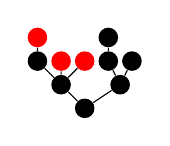
\begin{tikzpicture}[scale=.2]
\node[circle, scale=0.75, fill] (tid0) at (3.75,1.5){};
\node[circle, scale=0.75, fill] (tid1) at (2.25,3){};
\node[circle, scale=0.75, fill] (tid3) at (0.75,4.5){};
\node[circle, scale=0.75, fill, red] (tid8) at (0.75,6){};
\draw[](tid3) -- (tid8);
\node[circle, scale=0.75, fill, red] (tid4) at (2.25,4.5){};
\node[circle, scale=0.75, fill, red] (tid5) at (3.75,4.5){};
\draw[](tid1) -- (tid3);
\draw[](tid1) -- (tid4);
\draw[](tid1) -- (tid5);
\node[circle, scale=0.75, fill] (tid2) at (6,3){};
\node[circle, scale=0.75, fill] (tid6) at (5.25,4.5){};
\node[circle, scale=0.75, fill] (tid9) at (5.25,6){};
\draw[](tid6) -- (tid9);
\node[circle, scale=0.75, fill] (tid7) at (6.75,4.5){};
\draw[](tid2) -- (tid6);
\draw[](tid2) -- (tid7);
\draw[](tid0) -- (tid1);
\draw[](tid0) -- (tid2);
\end{tikzpicture}
\nodepart{three}
\footnotesize{5.61513}
\nodepart{four}
\footnotesize{$33\:33\:11\:11\:11$}
};
 & 
\node[draw=black, rectangle split,  rectangle split parts=4] (sn0x9ba1038){
\footnotesize{1.85185}
\nodepart{two}
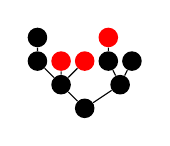
\begin{tikzpicture}[scale=.2]
\node[circle, scale=0.75, fill] (tid0) at (3.75,1.5){};
\node[circle, scale=0.75, fill] (tid1) at (2.25,3){};
\node[circle, scale=0.75, fill] (tid3) at (0.75,4.5){};
\node[circle, scale=0.75, fill] (tid8) at (0.75,6){};
\draw[](tid3) -- (tid8);
\node[circle, scale=0.75, fill, red] (tid4) at (2.25,4.5){};
\node[circle, scale=0.75, fill, red] (tid5) at (3.75,4.5){};
\draw[](tid1) -- (tid3);
\draw[](tid1) -- (tid4);
\draw[](tid1) -- (tid5);
\node[circle, scale=0.75, fill] (tid2) at (6,3){};
\node[circle, scale=0.75, fill] (tid6) at (5.25,4.5){};
\node[circle, scale=0.75, fill, red] (tid9) at (5.25,6){};
\draw[](tid6) -- (tid9);
\node[circle, scale=0.75, fill] (tid7) at (6.75,4.5){};
\draw[](tid2) -- (tid6);
\draw[](tid2) -- (tid7);
\draw[](tid0) -- (tid1);
\draw[](tid0) -- (tid2);
\end{tikzpicture}
\nodepart{three}
\footnotesize{5.6151}
\nodepart{four}
\footnotesize{$33\:33\:22\:11$}
};
 & 
\node[draw=black, rectangle split,  rectangle split parts=4] (sn0x9ba1d10){
\footnotesize{1.38889}
\nodepart{two}
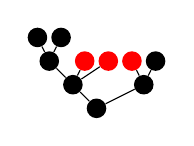
\begin{tikzpicture}[scale=.2]
\node[circle, scale=0.75, fill] (tid0) at (4.5,1.5){};
\node[circle, scale=0.75, fill] (tid1) at (3,3){};
\node[circle, scale=0.75, fill] (tid3) at (1.5,4.5){};
\node[circle, scale=0.75, fill] (tid8) at (0.75,6){};
\node[circle, scale=0.75, fill] (tid9) at (2.25,6){};
\draw[](tid3) -- (tid8);
\draw[](tid3) -- (tid9);
\node[circle, scale=0.75, fill, red] (tid4) at (3.75,4.5){};
\node[circle, scale=0.75, fill, red] (tid5) at (5.25,4.5){};
\draw[](tid1) -- (tid3);
\draw[](tid1) -- (tid4);
\draw[](tid1) -- (tid5);
\node[circle, scale=0.75, fill] (tid2) at (7.5,3){};
\node[circle, scale=0.75, fill, red] (tid6) at (6.75,4.5){};
\node[circle, scale=0.75, fill] (tid7) at (8.25,4.5){};
\draw[](tid2) -- (tid6);
\draw[](tid2) -- (tid7);
\draw[](tid0) -- (tid1);
\draw[](tid0) -- (tid2);
\end{tikzpicture}
\nodepart{three}
\footnotesize{5.70239}
\nodepart{four}
\footnotesize{$44\:22\:11\:22$}
};
 & 
\node[draw=black, rectangle split,  rectangle split parts=4] (sn0x9ba16b0){
\footnotesize{1.38889}
\nodepart{two}
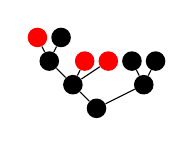
\begin{tikzpicture}[scale=.2]
\node[circle, scale=0.75, fill] (tid0) at (4.5,1.5){};
\node[circle, scale=0.75, fill] (tid1) at (3,3){};
\node[circle, scale=0.75, fill] (tid3) at (1.5,4.5){};
\node[circle, scale=0.75, fill, red] (tid8) at (0.75,6){};
\node[circle, scale=0.75, fill] (tid9) at (2.25,6){};
\draw[](tid3) -- (tid8);
\draw[](tid3) -- (tid9);
\node[circle, scale=0.75, fill, red] (tid4) at (3.75,4.5){};
\node[circle, scale=0.75, fill, red] (tid5) at (5.25,4.5){};
\draw[](tid1) -- (tid3);
\draw[](tid1) -- (tid4);
\draw[](tid1) -- (tid5);
\node[circle, scale=0.75, fill] (tid2) at (7.5,3){};
\node[circle, scale=0.75, fill] (tid6) at (6.75,4.5){};
\node[circle, scale=0.75, fill] (tid7) at (8.25,4.5){};
\draw[](tid2) -- (tid6);
\draw[](tid2) -- (tid7);
\draw[](tid0) -- (tid1);
\draw[](tid0) -- (tid2);
\end{tikzpicture}
\nodepart{three}
\footnotesize{5.61925}
\nodepart{four}
\footnotesize{$44\:22\:22\:11$}
};
 & 
\\
};
\end{scope}
\draw (sn0x9b87328.south) -- (sn0x9b9a400.north);
\draw (sn0x9b87328.south) -- (sn0x9b9aab0.north);
\draw (sn0x9b87328.south) -- (sn0x9b9ab88.north);
\draw (sn0x9b87328.south) -- (sn0x9b9a468.north);
\draw (sn0x9b87328.south) -- (sn0x9b9b1b8.north);
\draw (sn0x9b9a400.south) -- (sn0x9b9bcf0.north);
\draw (sn0x9b9a400.south) -- (sn0x9b8a418.north);
\draw (sn0x9b9a400.south) -- (sn0x9b9bb78.north);
\draw (sn0x9b9a400.south) -- (sn0x9b9c080.north);
\draw (sn0x9b9a400.south) -- (sn0x9b91878.north);
\draw (sn0x9b9a400.south) -- (sn0x9b9c560.north);
\draw (sn0x9b9a400.south) -- (sn0x9b8aa80.north);
\draw (sn0x9b9aab0.south) -- (sn0x9b9bcf0.north);
\draw (sn0x9b9aab0.south) -- (sn0x9b9dd18.north);
\draw (sn0x9b9aab0.south) -- (sn0x9b9c080.north);
\draw (sn0x9b9ab88.south) -- (sn0x9b9bb78.north);
\draw (sn0x9b9ab88.south) -- (sn0x9b9dd18.north);
\draw (sn0x9b9ab88.south) -- (sn0x9b9e468.north);
\draw (sn0x9b9ab88.south) -- (sn0x9b9db98.north);
\draw (sn0x9b9a468.south) -- (sn0x9b9bb78.north);
\draw (sn0x9b9a468.south) -- (sn0x9b91878.north);
\draw (sn0x9b9a468.south) -- (sn0x9b9c080.north);
\draw (sn0x9b9a468.south) -- (sn0x9ba10a0.north);
\draw (sn0x9b9a468.south) -- (sn0x9b97408.north);
\draw (sn0x9b9a468.south) -- (sn0x9ba1038.north);
\draw (sn0x9b9b1b8.south) -- (sn0x9b9dd18.north);
\draw (sn0x9b9b1b8.south) -- (sn0x9b9c080.north);
\draw (sn0x9b9b1b8.south) -- (sn0x9ba1d10.north);
\draw (sn0x9b9b1b8.south) -- (sn0x9ba16b0.north);
\end{tikzpicture}

%%% Local Variables:
%%% TeX-master: "thesis/thesis.tex"
%%% End: 
\renewcommand{\leveltopI}{-15cm + \leveltop}
\renewcommand{\leveltopII}{-15cm + \leveltopI}
\renewcommand{\leveltopIII}{-15cm + \leveltopII}
\renewcommand{\leveltopIIII}{-15cm + \leveltopIII}
\renewcommand{\leveltopIIIII}{-15cm + \leveltopIIII}
\renewcommand{\leveltopIIIIII}{-15cm + \leveltopIIIII}
\renewcommand{\leveltopIIIIIII}{-15cm + \leveltopIIIIII}
\renewcommand{\leveltopIIIIIIII}{-15cm + \leveltopIIIIIII}
\renewcommand{\leveltopIIIIIIIII}{-15cm + \leveltopIIIIIIII}
\renewcommand{\leveltopIIIIIIIIII}{-15cm + \leveltopIIIIIIIII}
\renewcommand{\leveltopIIIIIIIIIII}{-15cm + \leveltopIIIIIIIIII}
\renewcommand{\leveltopIIIIIIIIIIII}{-15cm + \leveltopIIIIIIIIIII}
\begin{tikzpicture}[scale=.2, anchor=south]
\begin{scope}[yshift=\leveltopI cm]
\matrix (line1)[column sep=1cm] {
\node[draw=black, rectangle split,  rectangle split parts=4] (sn0x9b877a8){
\footnotesize{100}
\nodepart{two}
\begin{tikzpicture}[scale=.2]
\node[circle, scale=0.75, fill] (tid0) at (4.5,1.5){};
\node[circle, scale=0.75, fill] (tid1) at (3,3){};
\node[circle, scale=0.75, fill] (tid3) at (1.5,4.5){};
\node[circle, scale=0.75, fill, red] (tid8) at (0.75,6){};
\node[circle, scale=0.75, fill] (tid9) at (2.25,6){};
\draw[](tid3) -- (tid8);
\draw[](tid3) -- (tid9);
\node[circle, scale=0.75, fill, red] (tid4) at (3.75,4.5){};
\node[circle, scale=0.75, fill, red] (tid5) at (5.25,4.5){};
\draw[](tid1) -- (tid3);
\draw[](tid1) -- (tid4);
\draw[](tid1) -- (tid5);
\node[circle, scale=0.75, fill] (tid2) at (7.5,3){};
\node[circle, scale=0.75, fill] (tid6) at (6.75,4.5){};
\node[circle, scale=0.75, fill] (tid10) at (6.75,6){};
\draw[](tid6) -- (tid10);
\node[circle, scale=0.75, fill] (tid7) at (8.25,4.5){};
\node[circle, scale=0.75, fill] (tid11) at (8.25,6){};
\draw[](tid7) -- (tid11);
\draw[](tid2) -- (tid6);
\draw[](tid2) -- (tid7);
\draw[](tid0) -- (tid1);
\draw[](tid0) -- (tid2);
\end{tikzpicture}
\nodepart{three}
\footnotesize{6.34718}
\nodepart{four}
\footnotesize{$22\:44\:11\:22$}
};
 & 
\\
};
\end{scope}
\begin{scope}[yshift=\leveltopII cm]
\matrix (line2)[column sep=1cm] {
\node[draw=black, rectangle split,  rectangle split parts=4] (sn0x9b89f18){
\footnotesize{22.2222}
\nodepart{two}
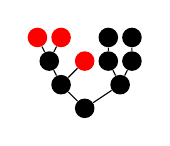
\begin{tikzpicture}[scale=.2]
\node[circle, scale=0.75, fill] (tid0) at (3.75,1.5){};
\node[circle, scale=0.75, fill] (tid1) at (2.25,3){};
\node[circle, scale=0.75, fill] (tid3) at (1.5,4.5){};
\node[circle, scale=0.75, fill, red] (tid7) at (0.75,6){};
\node[circle, scale=0.75, fill, red] (tid8) at (2.25,6){};
\draw[](tid3) -- (tid7);
\draw[](tid3) -- (tid8);
\node[circle, scale=0.75, fill, red] (tid4) at (3.75,4.5){};
\draw[](tid1) -- (tid3);
\draw[](tid1) -- (tid4);
\node[circle, scale=0.75, fill] (tid2) at (6,3){};
\node[circle, scale=0.75, fill] (tid5) at (5.25,4.5){};
\node[circle, scale=0.75, fill] (tid9) at (5.25,6){};
\draw[](tid5) -- (tid9);
\node[circle, scale=0.75, fill] (tid6) at (6.75,4.5){};
\node[circle, scale=0.75, fill] (tid10) at (6.75,6){};
\draw[](tid6) -- (tid10);
\draw[](tid2) -- (tid5);
\draw[](tid2) -- (tid6);
\draw[](tid0) -- (tid1);
\draw[](tid0) -- (tid2);
\end{tikzpicture}
\nodepart{three}
\footnotesize{6.01555}
\nodepart{four}
\footnotesize{$33\:67$}
};
 & 
\node[draw=black, rectangle split,  rectangle split parts=4] (sn0x9b9a400){
\footnotesize{44.4444}
\nodepart{two}
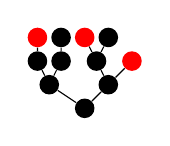
\begin{tikzpicture}[scale=.2]
\node[circle, scale=0.75, fill] (tid0) at (3.75,1.5){};
\node[circle, scale=0.75, fill] (tid1) at (1.5,3){};
\node[circle, scale=0.75, fill] (tid3) at (0.75,4.5){};
\node[circle, scale=0.75, fill, red] (tid7) at (0.75,6){};
\draw[](tid3) -- (tid7);
\node[circle, scale=0.75, fill] (tid4) at (2.25,4.5){};
\node[circle, scale=0.75, fill] (tid8) at (2.25,6){};
\draw[](tid4) -- (tid8);
\draw[](tid1) -- (tid3);
\draw[](tid1) -- (tid4);
\node[circle, scale=0.75, fill] (tid2) at (5.25,3){};
\node[circle, scale=0.75, fill] (tid5) at (4.5,4.5){};
\node[circle, scale=0.75, fill, red] (tid9) at (3.75,6){};
\node[circle, scale=0.75, fill] (tid10) at (5.25,6){};
\draw[](tid5) -- (tid9);
\draw[](tid5) -- (tid10);
\node[circle, scale=0.75, fill, red] (tid6) at (6.75,4.5){};
\draw[](tid2) -- (tid5);
\draw[](tid2) -- (tid6);
\draw[](tid0) -- (tid1);
\draw[](tid0) -- (tid2);
\end{tikzpicture}
\nodepart{three}
\footnotesize{6.03469}
\nodepart{four}
\footnotesize{$17\:17\:17\:11\:11\:11\:17$}
};
 & 
\node[draw=black, rectangle split,  rectangle split parts=4] (sn0x9b89cc0){
\footnotesize{11.1111}
\nodepart{two}
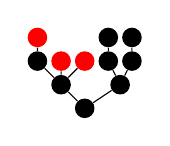
\begin{tikzpicture}[scale=.2]
\node[circle, scale=0.75, fill] (tid0) at (3.75,1.5){};
\node[circle, scale=0.75, fill] (tid1) at (2.25,3){};
\node[circle, scale=0.75, fill] (tid3) at (0.75,4.5){};
\node[circle, scale=0.75, fill, red] (tid8) at (0.75,6){};
\draw[](tid3) -- (tid8);
\node[circle, scale=0.75, fill, red] (tid4) at (2.25,4.5){};
\node[circle, scale=0.75, fill, red] (tid5) at (3.75,4.5){};
\draw[](tid1) -- (tid3);
\draw[](tid1) -- (tid4);
\draw[](tid1) -- (tid5);
\node[circle, scale=0.75, fill] (tid2) at (6,3){};
\node[circle, scale=0.75, fill] (tid6) at (5.25,4.5){};
\node[circle, scale=0.75, fill] (tid9) at (5.25,6){};
\draw[](tid6) -- (tid9);
\node[circle, scale=0.75, fill] (tid7) at (6.75,4.5){};
\node[circle, scale=0.75, fill] (tid10) at (6.75,6){};
\draw[](tid7) -- (tid10);
\draw[](tid2) -- (tid6);
\draw[](tid2) -- (tid7);
\draw[](tid0) -- (tid1);
\draw[](tid0) -- (tid2);
\end{tikzpicture}
\nodepart{three}
\footnotesize{5.97756}
\nodepart{four}
\footnotesize{$67\:11\:22$}
};
 & 
\node[draw=black, rectangle split,  rectangle split parts=4] (sn0x9ba1a80){
\footnotesize{22.2222}
\nodepart{two}
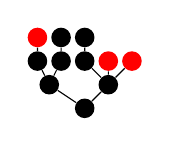
\begin{tikzpicture}[scale=.2]
\node[circle, scale=0.75, fill] (tid0) at (3.75,1.5){};
\node[circle, scale=0.75, fill] (tid1) at (1.5,3){};
\node[circle, scale=0.75, fill] (tid3) at (0.75,4.5){};
\node[circle, scale=0.75, fill, red] (tid8) at (0.75,6){};
\draw[](tid3) -- (tid8);
\node[circle, scale=0.75, fill] (tid4) at (2.25,4.5){};
\node[circle, scale=0.75, fill] (tid9) at (2.25,6){};
\draw[](tid4) -- (tid9);
\draw[](tid1) -- (tid3);
\draw[](tid1) -- (tid4);
\node[circle, scale=0.75, fill] (tid2) at (5.25,3){};
\node[circle, scale=0.75, fill] (tid5) at (3.75,4.5){};
\node[circle, scale=0.75, fill] (tid10) at (3.75,6){};
\draw[](tid5) -- (tid10);
\node[circle, scale=0.75, fill, red] (tid6) at (5.25,4.5){};
\node[circle, scale=0.75, fill, red] (tid7) at (6.75,4.5){};
\draw[](tid2) -- (tid5);
\draw[](tid2) -- (tid6);
\draw[](tid2) -- (tid7);
\draw[](tid0) -- (tid1);
\draw[](tid0) -- (tid2);
\end{tikzpicture}
\nodepart{three}
\footnotesize{5.9886}
\nodepart{four}
\footnotesize{$33\:33\:11\:11\:11$}
};
 & 
\\
};
\end{scope}
\begin{scope}[yshift=\leveltopIII cm]
\matrix (line3)[column sep=1cm] {
\node[draw=black, rectangle split,  rectangle split parts=4] (sn0x9b8a418){
\footnotesize{14.8148}
\nodepart{two}
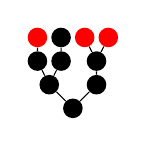
\begin{tikzpicture}[scale=.2]
\node[circle, scale=0.75, fill] (tid0) at (3,1.5){};
\node[circle, scale=0.75, fill] (tid1) at (1.5,3){};
\node[circle, scale=0.75, fill] (tid3) at (0.75,4.5){};
\node[circle, scale=0.75, fill, red] (tid6) at (0.75,6){};
\draw[](tid3) -- (tid6);
\node[circle, scale=0.75, fill] (tid4) at (2.25,4.5){};
\node[circle, scale=0.75, fill] (tid7) at (2.25,6){};
\draw[](tid4) -- (tid7);
\draw[](tid1) -- (tid3);
\draw[](tid1) -- (tid4);
\node[circle, scale=0.75, fill] (tid2) at (4.5,3){};
\node[circle, scale=0.75, fill] (tid5) at (4.5,4.5){};
\node[circle, scale=0.75, fill, red] (tid8) at (3.75,6){};
\node[circle, scale=0.75, fill, red] (tid9) at (5.25,6){};
\draw[](tid5) -- (tid8);
\draw[](tid5) -- (tid9);
\draw[](tid2) -- (tid5);
\draw[](tid0) -- (tid1);
\draw[](tid0) -- (tid2);
\end{tikzpicture}
\nodepart{three}
\footnotesize{5.7278}
\nodepart{four}
\footnotesize{$17\:17\:67$}
};
 & 
\node[draw=black, rectangle split,  rectangle split parts=4] (sn0x9b8aa80){
\footnotesize{37.037}
\nodepart{two}
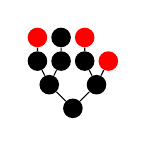
\begin{tikzpicture}[scale=.2]
\node[circle, scale=0.75, fill] (tid0) at (3,1.5){};
\node[circle, scale=0.75, fill] (tid1) at (1.5,3){};
\node[circle, scale=0.75, fill] (tid3) at (0.75,4.5){};
\node[circle, scale=0.75, fill, red] (tid7) at (0.75,6){};
\draw[](tid3) -- (tid7);
\node[circle, scale=0.75, fill] (tid4) at (2.25,4.5){};
\node[circle, scale=0.75, fill] (tid8) at (2.25,6){};
\draw[](tid4) -- (tid8);
\draw[](tid1) -- (tid3);
\draw[](tid1) -- (tid4);
\node[circle, scale=0.75, fill] (tid2) at (4.5,3){};
\node[circle, scale=0.75, fill] (tid5) at (3.75,4.5){};
\node[circle, scale=0.75, fill, red] (tid9) at (3.75,6){};
\draw[](tid5) -- (tid9);
\node[circle, scale=0.75, fill, red] (tid6) at (5.25,4.5){};
\draw[](tid2) -- (tid5);
\draw[](tid2) -- (tid6);
\draw[](tid0) -- (tid1);
\draw[](tid0) -- (tid2);
\end{tikzpicture}
\nodepart{three}
\footnotesize{5.65942}
\nodepart{four}
\footnotesize{$33\:17\:17\:17\:17$}
};
 & 
\node[draw=black, rectangle split,  rectangle split parts=4] (sn0x9b9bcf0){
\footnotesize{7.40741}
\nodepart{two}
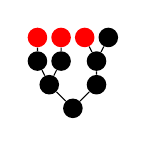
\begin{tikzpicture}[scale=.2]
\node[circle, scale=0.75, fill] (tid0) at (3,1.5){};
\node[circle, scale=0.75, fill] (tid1) at (1.5,3){};
\node[circle, scale=0.75, fill] (tid3) at (0.75,4.5){};
\node[circle, scale=0.75, fill, red] (tid6) at (0.75,6){};
\draw[](tid3) -- (tid6);
\node[circle, scale=0.75, fill] (tid4) at (2.25,4.5){};
\node[circle, scale=0.75, fill, red] (tid7) at (2.25,6){};
\draw[](tid4) -- (tid7);
\draw[](tid1) -- (tid3);
\draw[](tid1) -- (tid4);
\node[circle, scale=0.75, fill] (tid2) at (4.5,3){};
\node[circle, scale=0.75, fill] (tid5) at (4.5,4.5){};
\node[circle, scale=0.75, fill, red] (tid8) at (3.75,6){};
\node[circle, scale=0.75, fill] (tid9) at (5.25,6){};
\draw[](tid5) -- (tid8);
\draw[](tid5) -- (tid9);
\draw[](tid2) -- (tid5);
\draw[](tid0) -- (tid1);
\draw[](tid0) -- (tid2);
\end{tikzpicture}
\nodepart{three}
\footnotesize{5.74108}
\nodepart{four}
\footnotesize{$33\:33\:33$}
};
 & 
\node[draw=black, rectangle split,  rectangle split parts=4] (sn0x9b9bb78){
\footnotesize{4.93827}
\nodepart{two}
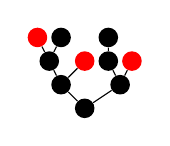
\begin{tikzpicture}[scale=.2]
\node[circle, scale=0.75, fill] (tid0) at (3.75,1.5){};
\node[circle, scale=0.75, fill] (tid1) at (2.25,3){};
\node[circle, scale=0.75, fill] (tid3) at (1.5,4.5){};
\node[circle, scale=0.75, fill, red] (tid7) at (0.75,6){};
\node[circle, scale=0.75, fill] (tid8) at (2.25,6){};
\draw[](tid3) -- (tid7);
\draw[](tid3) -- (tid8);
\node[circle, scale=0.75, fill, red] (tid4) at (3.75,4.5){};
\draw[](tid1) -- (tid3);
\draw[](tid1) -- (tid4);
\node[circle, scale=0.75, fill] (tid2) at (6,3){};
\node[circle, scale=0.75, fill] (tid5) at (5.25,4.5){};
\node[circle, scale=0.75, fill] (tid9) at (5.25,6){};
\draw[](tid5) -- (tid9);
\node[circle, scale=0.75, fill, red] (tid6) at (6.75,4.5){};
\draw[](tid2) -- (tid5);
\draw[](tid2) -- (tid6);
\draw[](tid0) -- (tid1);
\draw[](tid0) -- (tid2);
\end{tikzpicture}
\nodepart{three}
\footnotesize{5.75146}
\nodepart{four}
\footnotesize{$17\:33\:17\:17\:17$}
};
 & 
\node[draw=black, rectangle split,  rectangle split parts=4] (sn0x9b9c080){
\footnotesize{4.93827}
\nodepart{two}
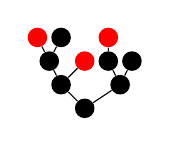
\begin{tikzpicture}[scale=.2]
\node[circle, scale=0.75, fill] (tid0) at (3.75,1.5){};
\node[circle, scale=0.75, fill] (tid1) at (2.25,3){};
\node[circle, scale=0.75, fill] (tid3) at (1.5,4.5){};
\node[circle, scale=0.75, fill, red] (tid7) at (0.75,6){};
\node[circle, scale=0.75, fill] (tid8) at (2.25,6){};
\draw[](tid3) -- (tid7);
\draw[](tid3) -- (tid8);
\node[circle, scale=0.75, fill, red] (tid4) at (3.75,4.5){};
\draw[](tid1) -- (tid3);
\draw[](tid1) -- (tid4);
\node[circle, scale=0.75, fill] (tid2) at (6,3){};
\node[circle, scale=0.75, fill] (tid5) at (5.25,4.5){};
\node[circle, scale=0.75, fill, red] (tid9) at (5.25,6){};
\draw[](tid5) -- (tid9);
\node[circle, scale=0.75, fill] (tid6) at (6.75,4.5){};
\draw[](tid2) -- (tid5);
\draw[](tid2) -- (tid6);
\draw[](tid0) -- (tid1);
\draw[](tid0) -- (tid2);
\end{tikzpicture}
\nodepart{three}
\footnotesize{5.68383}
\nodepart{four}
\footnotesize{$17\:17\:17\:17\:22\:11$}
};
 & 
\node[draw=black, rectangle split,  rectangle split parts=4] (sn0x9b91878){
\footnotesize{4.93827}
\nodepart{two}
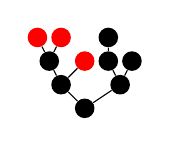
\begin{tikzpicture}[scale=.2]
\node[circle, scale=0.75, fill] (tid0) at (3.75,1.5){};
\node[circle, scale=0.75, fill] (tid1) at (2.25,3){};
\node[circle, scale=0.75, fill] (tid3) at (1.5,4.5){};
\node[circle, scale=0.75, fill, red] (tid7) at (0.75,6){};
\node[circle, scale=0.75, fill, red] (tid8) at (2.25,6){};
\draw[](tid3) -- (tid7);
\draw[](tid3) -- (tid8);
\node[circle, scale=0.75, fill, red] (tid4) at (3.75,4.5){};
\draw[](tid1) -- (tid3);
\draw[](tid1) -- (tid4);
\node[circle, scale=0.75, fill] (tid2) at (6,3){};
\node[circle, scale=0.75, fill] (tid5) at (5.25,4.5){};
\node[circle, scale=0.75, fill] (tid9) at (5.25,6){};
\draw[](tid5) -- (tid9);
\node[circle, scale=0.75, fill] (tid6) at (6.75,4.5){};
\draw[](tid2) -- (tid5);
\draw[](tid2) -- (tid6);
\draw[](tid0) -- (tid1);
\draw[](tid0) -- (tid2);
\end{tikzpicture}
\nodepart{three}
\footnotesize{5.68176}
\nodepart{four}
\footnotesize{$17\:17\:33\:33$}
};
 & 
\node[draw=black, rectangle split,  rectangle split parts=4] (sn0x9b9c560){
\footnotesize{14.8148}
\nodepart{two}
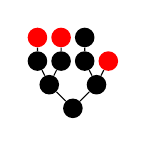
\begin{tikzpicture}[scale=.2]
\node[circle, scale=0.75, fill] (tid0) at (3,1.5){};
\node[circle, scale=0.75, fill] (tid1) at (1.5,3){};
\node[circle, scale=0.75, fill] (tid3) at (0.75,4.5){};
\node[circle, scale=0.75, fill, red] (tid7) at (0.75,6){};
\draw[](tid3) -- (tid7);
\node[circle, scale=0.75, fill] (tid4) at (2.25,4.5){};
\node[circle, scale=0.75, fill, red] (tid8) at (2.25,6){};
\draw[](tid4) -- (tid8);
\draw[](tid1) -- (tid3);
\draw[](tid1) -- (tid4);
\node[circle, scale=0.75, fill] (tid2) at (4.5,3){};
\node[circle, scale=0.75, fill] (tid5) at (3.75,4.5){};
\node[circle, scale=0.75, fill] (tid9) at (3.75,6){};
\draw[](tid5) -- (tid9);
\node[circle, scale=0.75, fill, red] (tid6) at (5.25,4.5){};
\draw[](tid2) -- (tid5);
\draw[](tid2) -- (tid6);
\draw[](tid0) -- (tid1);
\draw[](tid0) -- (tid2);
\end{tikzpicture}
\nodepart{three}
\footnotesize{5.66847}
\nodepart{four}
\footnotesize{$33\:33\:33$}
};
 & 
\node[draw=black, rectangle split,  rectangle split parts=4] (sn0x9b94588){
\footnotesize{1.23457}
\nodepart{two}
\begin{tikzpicture}[scale=.2]
\node[circle, scale=0.75, fill] (tid0) at (3.75,1.5){};
\node[circle, scale=0.75, fill] (tid1) at (1.5,3){};
\node[circle, scale=0.75, fill] (tid3) at (0.75,4.5){};
\node[circle, scale=0.75, fill] (tid8) at (0.75,6){};
\draw[](tid3) -- (tid8);
\node[circle, scale=0.75, fill] (tid4) at (2.25,4.5){};
\node[circle, scale=0.75, fill] (tid9) at (2.25,6){};
\draw[](tid4) -- (tid9);
\draw[](tid1) -- (tid3);
\draw[](tid1) -- (tid4);
\node[circle, scale=0.75, fill] (tid2) at (5.25,3){};
\node[circle, scale=0.75, fill, red] (tid5) at (3.75,4.5){};
\node[circle, scale=0.75, fill, red] (tid6) at (5.25,4.5){};
\node[circle, scale=0.75, fill, red] (tid7) at (6.75,4.5){};
\draw[](tid2) -- (tid5);
\draw[](tid2) -- (tid6);
\draw[](tid2) -- (tid7);
\draw[](tid0) -- (tid1);
\draw[](tid0) -- (tid2);
\end{tikzpicture}
\nodepart{three}
\footnotesize{5.64738}
\nodepart{four}
\footnotesize{$1$}
};
 & 
\node[draw=black, rectangle split,  rectangle split parts=4] (sn0x9b94698){
\footnotesize{2.46914}
\nodepart{two}
\begin{tikzpicture}[scale=.2]
\node[circle, scale=0.75, fill] (tid0) at (3.75,1.5){};
\node[circle, scale=0.75, fill] (tid1) at (1.5,3){};
\node[circle, scale=0.75, fill] (tid3) at (0.75,4.5){};
\node[circle, scale=0.75, fill, red] (tid8) at (0.75,6){};
\draw[](tid3) -- (tid8);
\node[circle, scale=0.75, fill] (tid4) at (2.25,4.5){};
\node[circle, scale=0.75, fill] (tid9) at (2.25,6){};
\draw[](tid4) -- (tid9);
\draw[](tid1) -- (tid3);
\draw[](tid1) -- (tid4);
\node[circle, scale=0.75, fill] (tid2) at (5.25,3){};
\node[circle, scale=0.75, fill, red] (tid5) at (3.75,4.5){};
\node[circle, scale=0.75, fill, red] (tid6) at (5.25,4.5){};
\node[circle, scale=0.75, fill] (tid7) at (6.75,4.5){};
\draw[](tid2) -- (tid5);
\draw[](tid2) -- (tid6);
\draw[](tid2) -- (tid7);
\draw[](tid0) -- (tid1);
\draw[](tid0) -- (tid2);
\end{tikzpicture}
\nodepart{three}
\footnotesize{5.59704}
\nodepart{four}
\footnotesize{$33\:33\:11\:11\:11$}
};
 & 
\node[draw=black, rectangle split,  rectangle split parts=4] (sn0x9ba10a0){
\footnotesize{2.46914}
\nodepart{two}
\begin{tikzpicture}[scale=.2]
\node[circle, scale=0.75, fill] (tid0) at (3.75,1.5){};
\node[circle, scale=0.75, fill] (tid1) at (2.25,3){};
\node[circle, scale=0.75, fill] (tid3) at (0.75,4.5){};
\node[circle, scale=0.75, fill] (tid8) at (0.75,6){};
\draw[](tid3) -- (tid8);
\node[circle, scale=0.75, fill, red] (tid4) at (2.25,4.5){};
\node[circle, scale=0.75, fill, red] (tid5) at (3.75,4.5){};
\draw[](tid1) -- (tid3);
\draw[](tid1) -- (tid4);
\draw[](tid1) -- (tid5);
\node[circle, scale=0.75, fill] (tid2) at (6,3){};
\node[circle, scale=0.75, fill] (tid6) at (5.25,4.5){};
\node[circle, scale=0.75, fill] (tid9) at (5.25,6){};
\draw[](tid6) -- (tid9);
\node[circle, scale=0.75, fill, red] (tid7) at (6.75,4.5){};
\draw[](tid2) -- (tid6);
\draw[](tid2) -- (tid7);
\draw[](tid0) -- (tid1);
\draw[](tid0) -- (tid2);
\end{tikzpicture}
\nodepart{three}
\footnotesize{5.68347}
\nodepart{four}
\footnotesize{$67\:17\:17$}
};
 & 
\node[draw=black, rectangle split,  rectangle split parts=4] (sn0x9ba1038){
\footnotesize{2.46914}
\nodepart{two}
\begin{tikzpicture}[scale=.2]
\node[circle, scale=0.75, fill] (tid0) at (3.75,1.5){};
\node[circle, scale=0.75, fill] (tid1) at (2.25,3){};
\node[circle, scale=0.75, fill] (tid3) at (0.75,4.5){};
\node[circle, scale=0.75, fill] (tid8) at (0.75,6){};
\draw[](tid3) -- (tid8);
\node[circle, scale=0.75, fill, red] (tid4) at (2.25,4.5){};
\node[circle, scale=0.75, fill, red] (tid5) at (3.75,4.5){};
\draw[](tid1) -- (tid3);
\draw[](tid1) -- (tid4);
\draw[](tid1) -- (tid5);
\node[circle, scale=0.75, fill] (tid2) at (6,3){};
\node[circle, scale=0.75, fill] (tid6) at (5.25,4.5){};
\node[circle, scale=0.75, fill, red] (tid9) at (5.25,6){};
\draw[](tid6) -- (tid9);
\node[circle, scale=0.75, fill] (tid7) at (6.75,4.5){};
\draw[](tid2) -- (tid6);
\draw[](tid2) -- (tid7);
\draw[](tid0) -- (tid1);
\draw[](tid0) -- (tid2);
\end{tikzpicture}
\nodepart{three}
\footnotesize{5.6151}
\nodepart{four}
\footnotesize{$33\:33\:22\:11$}
};
 & 
\node[draw=black, rectangle split,  rectangle split parts=4] (sn0x9b97408){
\footnotesize{2.46914}
\nodepart{two}
\begin{tikzpicture}[scale=.2]
\node[circle, scale=0.75, fill] (tid0) at (3.75,1.5){};
\node[circle, scale=0.75, fill] (tid1) at (2.25,3){};
\node[circle, scale=0.75, fill] (tid3) at (0.75,4.5){};
\node[circle, scale=0.75, fill, red] (tid8) at (0.75,6){};
\draw[](tid3) -- (tid8);
\node[circle, scale=0.75, fill, red] (tid4) at (2.25,4.5){};
\node[circle, scale=0.75, fill, red] (tid5) at (3.75,4.5){};
\draw[](tid1) -- (tid3);
\draw[](tid1) -- (tid4);
\draw[](tid1) -- (tid5);
\node[circle, scale=0.75, fill] (tid2) at (6,3){};
\node[circle, scale=0.75, fill] (tid6) at (5.25,4.5){};
\node[circle, scale=0.75, fill] (tid9) at (5.25,6){};
\draw[](tid6) -- (tid9);
\node[circle, scale=0.75, fill] (tid7) at (6.75,4.5){};
\draw[](tid2) -- (tid6);
\draw[](tid2) -- (tid7);
\draw[](tid0) -- (tid1);
\draw[](tid0) -- (tid2);
\end{tikzpicture}
\nodepart{three}
\footnotesize{5.61513}
\nodepart{four}
\footnotesize{$33\:33\:11\:11\:11$}
};
 & 
\\
};
\end{scope}
\draw (sn0x9b877a8.south) -- (sn0x9b89f18.north);
\draw (sn0x9b877a8.south) -- (sn0x9b9a400.north);
\draw (sn0x9b877a8.south) -- (sn0x9b89cc0.north);
\draw (sn0x9b877a8.south) -- (sn0x9ba1a80.north);
\draw (sn0x9b89f18.south) -- (sn0x9b8a418.north);
\draw (sn0x9b89f18.south) -- (sn0x9b8aa80.north);
\draw (sn0x9b9a400.south) -- (sn0x9b9bcf0.north);
\draw (sn0x9b9a400.south) -- (sn0x9b8a418.north);
\draw (sn0x9b9a400.south) -- (sn0x9b9bb78.north);
\draw (sn0x9b9a400.south) -- (sn0x9b9c080.north);
\draw (sn0x9b9a400.south) -- (sn0x9b91878.north);
\draw (sn0x9b9a400.south) -- (sn0x9b9c560.north);
\draw (sn0x9b9a400.south) -- (sn0x9b8aa80.north);
\draw (sn0x9b89cc0.south) -- (sn0x9b8aa80.north);
\draw (sn0x9b89cc0.south) -- (sn0x9b94588.north);
\draw (sn0x9b89cc0.south) -- (sn0x9b94698.north);
\draw (sn0x9ba1a80.south) -- (sn0x9b9c560.north);
\draw (sn0x9ba1a80.south) -- (sn0x9b8aa80.north);
\draw (sn0x9ba1a80.south) -- (sn0x9ba10a0.north);
\draw (sn0x9ba1a80.south) -- (sn0x9ba1038.north);
\draw (sn0x9ba1a80.south) -- (sn0x9b97408.north);
\end{tikzpicture}

%%% Local Variables:
%%% TeX-master: "thesis/thesis.tex"
%%% End: 
\renewcommand{\leveltopI}{-15cm + \leveltop}
\renewcommand{\leveltopII}{-15cm + \leveltopI}
\renewcommand{\leveltopIII}{-15cm + \leveltopII}
\renewcommand{\leveltopIIII}{-15cm + \leveltopIII}
\renewcommand{\leveltopIIIII}{-15cm + \leveltopIIII}
\renewcommand{\leveltopIIIIII}{-15cm + \leveltopIIIII}
\renewcommand{\leveltopIIIIIII}{-15cm + \leveltopIIIIII}
\renewcommand{\leveltopIIIIIIII}{-15cm + \leveltopIIIIIII}
\renewcommand{\leveltopIIIIIIIII}{-15cm + \leveltopIIIIIIII}
\renewcommand{\leveltopIIIIIIIIII}{-15cm + \leveltopIIIIIIIII}
\renewcommand{\leveltopIIIIIIIIIII}{-15cm + \leveltopIIIIIIIIII}
\renewcommand{\leveltopIIIIIIIIIIII}{-15cm + \leveltopIIIIIIIIIII}
\begin{tikzpicture}[scale=.2, anchor=south]
\begin{scope}[yshift=\leveltopI cm]
\matrix (line1)[column sep=1cm] {
\node[draw=black, rectangle split,  rectangle split parts=4] (sn0x9b87c10){
\footnotesize{100}
\nodepart{two}
\begin{tikzpicture}[scale=.2]
\node[circle, scale=0.75, fill] (tid0) at (4.5,1.5){};
\node[circle, scale=0.75, fill] (tid1) at (3,3){};
\node[circle, scale=0.75, fill] (tid3) at (1.5,4.5){};
\node[circle, scale=0.75, fill] (tid8) at (0.75,6){};
\node[circle, scale=0.75, fill] (tid9) at (2.25,6){};
\draw[](tid3) -- (tid8);
\draw[](tid3) -- (tid9);
\node[circle, scale=0.75, fill, red] (tid4) at (3.75,4.5){};
\node[circle, scale=0.75, fill] (tid5) at (5.25,4.5){};
\draw[](tid1) -- (tid3);
\draw[](tid1) -- (tid4);
\draw[](tid1) -- (tid5);
\node[circle, scale=0.75, fill] (tid2) at (7.5,3){};
\node[circle, scale=0.75, fill] (tid6) at (6.75,4.5){};
\node[circle, scale=0.75, fill, red] (tid10) at (6.75,6){};
\draw[](tid6) -- (tid10);
\node[circle, scale=0.75, fill] (tid7) at (8.25,4.5){};
\node[circle, scale=0.75, fill, red] (tid11) at (8.25,6){};
\draw[](tid7) -- (tid11);
\draw[](tid2) -- (tid6);
\draw[](tid2) -- (tid7);
\draw[](tid0) -- (tid1);
\draw[](tid0) -- (tid2);
\end{tikzpicture}
\nodepart{three}
\footnotesize{6.32439}
\nodepart{four}
\footnotesize{$11\:22\:17\:17\:33$}
};
 & 
\\
};
\end{scope}
\begin{scope}[yshift=\leveltopII cm]
\matrix (line2)[column sep=1cm] {
\node[draw=black, rectangle split,  rectangle split parts=4] (sn0x9b9aab0){
\footnotesize{11.1111}
\nodepart{two}
\begin{tikzpicture}[scale=.2]
\node[circle, scale=0.75, fill] (tid0) at (3.75,1.5){};
\node[circle, scale=0.75, fill] (tid1) at (1.5,3){};
\node[circle, scale=0.75, fill] (tid3) at (0.75,4.5){};
\node[circle, scale=0.75, fill, red] (tid7) at (0.75,6){};
\draw[](tid3) -- (tid7);
\node[circle, scale=0.75, fill] (tid4) at (2.25,4.5){};
\node[circle, scale=0.75, fill, red] (tid8) at (2.25,6){};
\draw[](tid4) -- (tid8);
\draw[](tid1) -- (tid3);
\draw[](tid1) -- (tid4);
\node[circle, scale=0.75, fill] (tid2) at (5.25,3){};
\node[circle, scale=0.75, fill] (tid5) at (4.5,4.5){};
\node[circle, scale=0.75, fill] (tid9) at (3.75,6){};
\node[circle, scale=0.75, fill] (tid10) at (5.25,6){};
\draw[](tid5) -- (tid9);
\draw[](tid5) -- (tid10);
\node[circle, scale=0.75, fill, red] (tid6) at (6.75,4.5){};
\draw[](tid2) -- (tid5);
\draw[](tid2) -- (tid6);
\draw[](tid0) -- (tid1);
\draw[](tid0) -- (tid2);
\end{tikzpicture}
\nodepart{three}
\footnotesize{6.05253}
\nodepart{four}
\footnotesize{$33\:22\:44$}
};
 & 
\node[draw=black, rectangle split,  rectangle split parts=4] (sn0x9ba2b68){
\footnotesize{22.2222}
\nodepart{two}
\begin{tikzpicture}[scale=.2]
\node[circle, scale=0.75, fill] (tid0) at (3.75,1.5){};
\node[circle, scale=0.75, fill] (tid1) at (1.5,3){};
\node[circle, scale=0.75, fill] (tid3) at (0.75,4.5){};
\node[circle, scale=0.75, fill, red] (tid7) at (0.75,6){};
\draw[](tid3) -- (tid7);
\node[circle, scale=0.75, fill] (tid4) at (2.25,4.5){};
\node[circle, scale=0.75, fill, red] (tid8) at (2.25,6){};
\draw[](tid4) -- (tid8);
\draw[](tid1) -- (tid3);
\draw[](tid1) -- (tid4);
\node[circle, scale=0.75, fill] (tid2) at (5.25,3){};
\node[circle, scale=0.75, fill] (tid5) at (4.5,4.5){};
\node[circle, scale=0.75, fill, red] (tid9) at (3.75,6){};
\node[circle, scale=0.75, fill] (tid10) at (5.25,6){};
\draw[](tid5) -- (tid9);
\draw[](tid5) -- (tid10);
\node[circle, scale=0.75, fill] (tid6) at (6.75,4.5){};
\draw[](tid2) -- (tid5);
\draw[](tid2) -- (tid6);
\draw[](tid0) -- (tid1);
\draw[](tid0) -- (tid2);
\end{tikzpicture}
\nodepart{three}
\footnotesize{5.98166}
\nodepart{four}
\footnotesize{$22\:22\:22\:17\:17$}
};
 & 
\node[draw=black, rectangle split,  rectangle split parts=4] (sn0x9b9b1b8){
\footnotesize{16.6667}
\nodepart{two}
\begin{tikzpicture}[scale=.2]
\node[circle, scale=0.75, fill] (tid0) at (4.5,1.5){};
\node[circle, scale=0.75, fill] (tid1) at (3,3){};
\node[circle, scale=0.75, fill] (tid3) at (1.5,4.5){};
\node[circle, scale=0.75, fill] (tid8) at (0.75,6){};
\node[circle, scale=0.75, fill] (tid9) at (2.25,6){};
\draw[](tid3) -- (tid8);
\draw[](tid3) -- (tid9);
\node[circle, scale=0.75, fill, red] (tid4) at (3.75,4.5){};
\node[circle, scale=0.75, fill, red] (tid5) at (5.25,4.5){};
\draw[](tid1) -- (tid3);
\draw[](tid1) -- (tid4);
\draw[](tid1) -- (tid5);
\node[circle, scale=0.75, fill] (tid2) at (7.5,3){};
\node[circle, scale=0.75, fill] (tid6) at (6.75,4.5){};
\node[circle, scale=0.75, fill, red] (tid10) at (6.75,6){};
\draw[](tid6) -- (tid10);
\node[circle, scale=0.75, fill] (tid7) at (8.25,4.5){};
\draw[](tid2) -- (tid6);
\draw[](tid2) -- (tid7);
\draw[](tid0) -- (tid1);
\draw[](tid0) -- (tid2);
\end{tikzpicture}
\nodepart{three}
\footnotesize{6.02577}
\nodepart{four}
\footnotesize{$22\:44\:17\:17$}
};
 & 
\node[draw=black, rectangle split,  rectangle split parts=4] (sn0x9ba2bd0){
\footnotesize{16.6667}
\nodepart{two}
\begin{tikzpicture}[scale=.2]
\node[circle, scale=0.75, fill] (tid0) at (4.5,1.5){};
\node[circle, scale=0.75, fill] (tid1) at (3,3){};
\node[circle, scale=0.75, fill] (tid3) at (1.5,4.5){};
\node[circle, scale=0.75, fill] (tid8) at (0.75,6){};
\node[circle, scale=0.75, fill] (tid9) at (2.25,6){};
\draw[](tid3) -- (tid8);
\draw[](tid3) -- (tid9);
\node[circle, scale=0.75, fill, red] (tid4) at (3.75,4.5){};
\node[circle, scale=0.75, fill] (tid5) at (5.25,4.5){};
\draw[](tid1) -- (tid3);
\draw[](tid1) -- (tid4);
\draw[](tid1) -- (tid5);
\node[circle, scale=0.75, fill] (tid2) at (7.5,3){};
\node[circle, scale=0.75, fill] (tid6) at (6.75,4.5){};
\node[circle, scale=0.75, fill, red] (tid10) at (6.75,6){};
\draw[](tid6) -- (tid10);
\node[circle, scale=0.75, fill, red] (tid7) at (8.25,4.5){};
\draw[](tid2) -- (tid6);
\draw[](tid2) -- (tid7);
\draw[](tid0) -- (tid1);
\draw[](tid0) -- (tid2);
\end{tikzpicture}
\nodepart{three}
\footnotesize{6.02153}
\nodepart{four}
\footnotesize{$11\:22\:8.3\:11\:22\:8.3\:17$}
};
 & 
\node[draw=black, rectangle split,  rectangle split parts=4] (sn0x9ba2920){
\footnotesize{33.3333}
\nodepart{two}
\begin{tikzpicture}[scale=.2]
\node[circle, scale=0.75, fill] (tid0) at (4.5,1.5){};
\node[circle, scale=0.75, fill] (tid1) at (3,3){};
\node[circle, scale=0.75, fill] (tid3) at (1.5,4.5){};
\node[circle, scale=0.75, fill, red] (tid8) at (0.75,6){};
\node[circle, scale=0.75, fill] (tid9) at (2.25,6){};
\draw[](tid3) -- (tid8);
\draw[](tid3) -- (tid9);
\node[circle, scale=0.75, fill, red] (tid4) at (3.75,4.5){};
\node[circle, scale=0.75, fill] (tid5) at (5.25,4.5){};
\draw[](tid1) -- (tid3);
\draw[](tid1) -- (tid4);
\draw[](tid1) -- (tid5);
\node[circle, scale=0.75, fill] (tid2) at (7.5,3){};
\node[circle, scale=0.75, fill] (tid6) at (6.75,4.5){};
\node[circle, scale=0.75, fill, red] (tid10) at (6.75,6){};
\draw[](tid6) -- (tid10);
\node[circle, scale=0.75, fill] (tid7) at (8.25,4.5){};
\draw[](tid2) -- (tid6);
\draw[](tid2) -- (tid7);
\draw[](tid0) -- (tid1);
\draw[](tid0) -- (tid2);
\end{tikzpicture}
\nodepart{three}
\footnotesize{5.94423}
\nodepart{four}
\footnotesize{$11\:11\:11\:8.3\:17\:11\:11\:11\:8.3$}
};
 & 
\\
};
\end{scope}
\begin{scope}[yshift=\leveltopIII cm]
\matrix (line3)[column sep=1cm] {
\node[draw=black, rectangle split,  rectangle split parts=4] (sn0x9b9bcf0){
\footnotesize{3.7037}
\nodepart{two}
\begin{tikzpicture}[scale=.2]
\node[circle, scale=0.75, fill] (tid0) at (3,1.5){};
\node[circle, scale=0.75, fill] (tid1) at (1.5,3){};
\node[circle, scale=0.75, fill] (tid3) at (0.75,4.5){};
\node[circle, scale=0.75, fill, red] (tid6) at (0.75,6){};
\draw[](tid3) -- (tid6);
\node[circle, scale=0.75, fill] (tid4) at (2.25,4.5){};
\node[circle, scale=0.75, fill, red] (tid7) at (2.25,6){};
\draw[](tid4) -- (tid7);
\draw[](tid1) -- (tid3);
\draw[](tid1) -- (tid4);
\node[circle, scale=0.75, fill] (tid2) at (4.5,3){};
\node[circle, scale=0.75, fill] (tid5) at (4.5,4.5){};
\node[circle, scale=0.75, fill, red] (tid8) at (3.75,6){};
\node[circle, scale=0.75, fill] (tid9) at (5.25,6){};
\draw[](tid5) -- (tid8);
\draw[](tid5) -- (tid9);
\draw[](tid2) -- (tid5);
\draw[](tid0) -- (tid1);
\draw[](tid0) -- (tid2);
\end{tikzpicture}
\nodepart{three}
\footnotesize{5.74108}
\nodepart{four}
\footnotesize{$33\:33\:33$}
};
 & 
\node[draw=black, rectangle split,  rectangle split parts=4] (sn0x9b9dd18){
\footnotesize{8.02469}
\nodepart{two}
\begin{tikzpicture}[scale=.2]
\node[circle, scale=0.75, fill] (tid0) at (3.75,1.5){};
\node[circle, scale=0.75, fill] (tid1) at (2.25,3){};
\node[circle, scale=0.75, fill] (tid3) at (1.5,4.5){};
\node[circle, scale=0.75, fill] (tid7) at (0.75,6){};
\node[circle, scale=0.75, fill] (tid8) at (2.25,6){};
\draw[](tid3) -- (tid7);
\draw[](tid3) -- (tid8);
\node[circle, scale=0.75, fill, red] (tid4) at (3.75,4.5){};
\draw[](tid1) -- (tid3);
\draw[](tid1) -- (tid4);
\node[circle, scale=0.75, fill] (tid2) at (6,3){};
\node[circle, scale=0.75, fill] (tid5) at (5.25,4.5){};
\node[circle, scale=0.75, fill, red] (tid9) at (5.25,6){};
\draw[](tid5) -- (tid9);
\node[circle, scale=0.75, fill, red] (tid6) at (6.75,4.5){};
\draw[](tid2) -- (tid5);
\draw[](tid2) -- (tid6);
\draw[](tid0) -- (tid1);
\draw[](tid0) -- (tid2);
\end{tikzpicture}
\nodepart{three}
\footnotesize{5.75709}
\nodepart{four}
\footnotesize{$33\:33\:11\:22$}
};
 & 
\node[draw=black, rectangle split,  rectangle split parts=4] (sn0x9b9c080){
\footnotesize{20.9877}
\nodepart{two}
\begin{tikzpicture}[scale=.2]
\node[circle, scale=0.75, fill] (tid0) at (3.75,1.5){};
\node[circle, scale=0.75, fill] (tid1) at (2.25,3){};
\node[circle, scale=0.75, fill] (tid3) at (1.5,4.5){};
\node[circle, scale=0.75, fill, red] (tid7) at (0.75,6){};
\node[circle, scale=0.75, fill] (tid8) at (2.25,6){};
\draw[](tid3) -- (tid7);
\draw[](tid3) -- (tid8);
\node[circle, scale=0.75, fill, red] (tid4) at (3.75,4.5){};
\draw[](tid1) -- (tid3);
\draw[](tid1) -- (tid4);
\node[circle, scale=0.75, fill] (tid2) at (6,3){};
\node[circle, scale=0.75, fill] (tid5) at (5.25,4.5){};
\node[circle, scale=0.75, fill, red] (tid9) at (5.25,6){};
\draw[](tid5) -- (tid9);
\node[circle, scale=0.75, fill] (tid6) at (6.75,4.5){};
\draw[](tid2) -- (tid5);
\draw[](tid2) -- (tid6);
\draw[](tid0) -- (tid1);
\draw[](tid0) -- (tid2);
\end{tikzpicture}
\nodepart{three}
\footnotesize{5.68383}
\nodepart{four}
\footnotesize{$17\:17\:22\:17\:17\:11$}
};
 & 
\node[draw=black, rectangle split,  rectangle split parts=4] (sn0x9ba3448){
\footnotesize{12.3457}
\nodepart{two}
\begin{tikzpicture}[scale=.2]
\node[circle, scale=0.75, fill] (tid0) at (3.75,1.5){};
\node[circle, scale=0.75, fill] (tid1) at (2.25,3){};
\node[circle, scale=0.75, fill] (tid3) at (1.5,4.5){};
\node[circle, scale=0.75, fill, red] (tid7) at (0.75,6){};
\node[circle, scale=0.75, fill] (tid8) at (2.25,6){};
\draw[](tid3) -- (tid7);
\draw[](tid3) -- (tid8);
\node[circle, scale=0.75, fill] (tid4) at (3.75,4.5){};
\draw[](tid1) -- (tid3);
\draw[](tid1) -- (tid4);
\node[circle, scale=0.75, fill] (tid2) at (6,3){};
\node[circle, scale=0.75, fill] (tid5) at (5.25,4.5){};
\node[circle, scale=0.75, fill, red] (tid9) at (5.25,6){};
\draw[](tid5) -- (tid9);
\node[circle, scale=0.75, fill, red] (tid6) at (6.75,4.5){};
\draw[](tid2) -- (tid5);
\draw[](tid2) -- (tid6);
\draw[](tid0) -- (tid1);
\draw[](tid0) -- (tid2);
\end{tikzpicture}
\nodepart{three}
\footnotesize{5.67863}
\nodepart{four}
\footnotesize{$17\:11\:17\:17\:17\:11\:11$}
};
 & 
\node[draw=black, rectangle split,  rectangle split parts=4] (sn0x9b91ba0){
\footnotesize{8.64198}
\nodepart{two}
\begin{tikzpicture}[scale=.2]
\node[circle, scale=0.75, fill] (tid0) at (3.75,1.5){};
\node[circle, scale=0.75, fill] (tid1) at (2.25,3){};
\node[circle, scale=0.75, fill] (tid3) at (1.5,4.5){};
\node[circle, scale=0.75, fill, red] (tid7) at (0.75,6){};
\node[circle, scale=0.75, fill, red] (tid8) at (2.25,6){};
\draw[](tid3) -- (tid7);
\draw[](tid3) -- (tid8);
\node[circle, scale=0.75, fill] (tid4) at (3.75,4.5){};
\draw[](tid1) -- (tid3);
\draw[](tid1) -- (tid4);
\node[circle, scale=0.75, fill] (tid2) at (6,3){};
\node[circle, scale=0.75, fill] (tid5) at (5.25,4.5){};
\node[circle, scale=0.75, fill, red] (tid9) at (5.25,6){};
\draw[](tid5) -- (tid9);
\node[circle, scale=0.75, fill] (tid6) at (6.75,4.5){};
\draw[](tid2) -- (tid5);
\draw[](tid2) -- (tid6);
\draw[](tid0) -- (tid1);
\draw[](tid0) -- (tid2);
\end{tikzpicture}
\nodepart{three}
\footnotesize{5.6024}
\nodepart{four}
\footnotesize{$67\:11\:22$}
};
 & 
\node[draw=black, rectangle split,  rectangle split parts=4] (sn0x9b9c560){
\footnotesize{3.7037}
\nodepart{two}
\begin{tikzpicture}[scale=.2]
\node[circle, scale=0.75, fill] (tid0) at (3,1.5){};
\node[circle, scale=0.75, fill] (tid1) at (1.5,3){};
\node[circle, scale=0.75, fill] (tid3) at (0.75,4.5){};
\node[circle, scale=0.75, fill, red] (tid7) at (0.75,6){};
\draw[](tid3) -- (tid7);
\node[circle, scale=0.75, fill] (tid4) at (2.25,4.5){};
\node[circle, scale=0.75, fill, red] (tid8) at (2.25,6){};
\draw[](tid4) -- (tid8);
\draw[](tid1) -- (tid3);
\draw[](tid1) -- (tid4);
\node[circle, scale=0.75, fill] (tid2) at (4.5,3){};
\node[circle, scale=0.75, fill] (tid5) at (3.75,4.5){};
\node[circle, scale=0.75, fill] (tid9) at (3.75,6){};
\draw[](tid5) -- (tid9);
\node[circle, scale=0.75, fill, red] (tid6) at (5.25,4.5){};
\draw[](tid2) -- (tid5);
\draw[](tid2) -- (tid6);
\draw[](tid0) -- (tid1);
\draw[](tid0) -- (tid2);
\end{tikzpicture}
\nodepart{three}
\footnotesize{5.66847}
\nodepart{four}
\footnotesize{$33\:33\:33$}
};
 & 
\node[draw=black, rectangle split,  rectangle split parts=4] (sn0x9b92190){
\footnotesize{3.7037}
\nodepart{two}
\begin{tikzpicture}[scale=.2]
\node[circle, scale=0.75, fill] (tid0) at (3,1.5){};
\node[circle, scale=0.75, fill] (tid1) at (1.5,3){};
\node[circle, scale=0.75, fill] (tid3) at (0.75,4.5){};
\node[circle, scale=0.75, fill, red] (tid7) at (0.75,6){};
\draw[](tid3) -- (tid7);
\node[circle, scale=0.75, fill] (tid4) at (2.25,4.5){};
\node[circle, scale=0.75, fill, red] (tid8) at (2.25,6){};
\draw[](tid4) -- (tid8);
\draw[](tid1) -- (tid3);
\draw[](tid1) -- (tid4);
\node[circle, scale=0.75, fill] (tid2) at (4.5,3){};
\node[circle, scale=0.75, fill] (tid5) at (3.75,4.5){};
\node[circle, scale=0.75, fill, red] (tid9) at (3.75,6){};
\draw[](tid5) -- (tid9);
\node[circle, scale=0.75, fill] (tid6) at (5.25,4.5){};
\draw[](tid2) -- (tid5);
\draw[](tid2) -- (tid6);
\draw[](tid0) -- (tid1);
\draw[](tid0) -- (tid2);
\end{tikzpicture}
\nodepart{three}
\footnotesize{5.60168}
\nodepart{four}
\footnotesize{$67\:33$}
};
 & 
\node[draw=black, rectangle split,  rectangle split parts=4] (sn0x9ba1d10){
\footnotesize{4.16667}
\nodepart{two}
\begin{tikzpicture}[scale=.2]
\node[circle, scale=0.75, fill] (tid0) at (4.5,1.5){};
\node[circle, scale=0.75, fill] (tid1) at (3,3){};
\node[circle, scale=0.75, fill] (tid3) at (1.5,4.5){};
\node[circle, scale=0.75, fill] (tid8) at (0.75,6){};
\node[circle, scale=0.75, fill] (tid9) at (2.25,6){};
\draw[](tid3) -- (tid8);
\draw[](tid3) -- (tid9);
\node[circle, scale=0.75, fill, red] (tid4) at (3.75,4.5){};
\node[circle, scale=0.75, fill, red] (tid5) at (5.25,4.5){};
\draw[](tid1) -- (tid3);
\draw[](tid1) -- (tid4);
\draw[](tid1) -- (tid5);
\node[circle, scale=0.75, fill] (tid2) at (7.5,3){};
\node[circle, scale=0.75, fill, red] (tid6) at (6.75,4.5){};
\node[circle, scale=0.75, fill] (tid7) at (8.25,4.5){};
\draw[](tid2) -- (tid6);
\draw[](tid2) -- (tid7);
\draw[](tid0) -- (tid1);
\draw[](tid0) -- (tid2);
\end{tikzpicture}
\nodepart{three}
\footnotesize{5.70239}
\nodepart{four}
\footnotesize{$22\:44\:11\:22$}
};
 & 
\node[draw=black, rectangle split,  rectangle split parts=4] (sn0x9ba16b0){
\footnotesize{5.55556}
\nodepart{two}
\begin{tikzpicture}[scale=.2]
\node[circle, scale=0.75, fill] (tid0) at (4.5,1.5){};
\node[circle, scale=0.75, fill] (tid1) at (3,3){};
\node[circle, scale=0.75, fill] (tid3) at (1.5,4.5){};
\node[circle, scale=0.75, fill, red] (tid8) at (0.75,6){};
\node[circle, scale=0.75, fill] (tid9) at (2.25,6){};
\draw[](tid3) -- (tid8);
\draw[](tid3) -- (tid9);
\node[circle, scale=0.75, fill, red] (tid4) at (3.75,4.5){};
\node[circle, scale=0.75, fill, red] (tid5) at (5.25,4.5){};
\draw[](tid1) -- (tid3);
\draw[](tid1) -- (tid4);
\draw[](tid1) -- (tid5);
\node[circle, scale=0.75, fill] (tid2) at (7.5,3){};
\node[circle, scale=0.75, fill] (tid6) at (6.75,4.5){};
\node[circle, scale=0.75, fill] (tid7) at (8.25,4.5){};
\draw[](tid2) -- (tid6);
\draw[](tid2) -- (tid7);
\draw[](tid0) -- (tid1);
\draw[](tid0) -- (tid2);
\end{tikzpicture}
\nodepart{three}
\footnotesize{5.61925}
\nodepart{four}
\footnotesize{$44\:22\:22\:11$}
};
 & 
\node[draw=black, rectangle split,  rectangle split parts=4] (sn0x9b9db98){
\footnotesize{1.85185}
\nodepart{two}
\begin{tikzpicture}[scale=.2]
\node[circle, scale=0.75, fill] (tid0) at (3.75,1.5){};
\node[circle, scale=0.75, fill] (tid1) at (3,3){};
\node[circle, scale=0.75, fill] (tid3) at (1.5,4.5){};
\node[circle, scale=0.75, fill] (tid7) at (0.75,6){};
\node[circle, scale=0.75, fill] (tid8) at (2.25,6){};
\draw[](tid3) -- (tid7);
\draw[](tid3) -- (tid8);
\node[circle, scale=0.75, fill, red] (tid4) at (3.75,4.5){};
\node[circle, scale=0.75, fill, red] (tid5) at (5.25,4.5){};
\draw[](tid1) -- (tid3);
\draw[](tid1) -- (tid4);
\draw[](tid1) -- (tid5);
\node[circle, scale=0.75, fill] (tid2) at (6.75,3){};
\node[circle, scale=0.75, fill] (tid6) at (6.75,4.5){};
\node[circle, scale=0.75, fill, red] (tid9) at (6.75,6){};
\draw[](tid6) -- (tid9);
\draw[](tid2) -- (tid6);
\draw[](tid0) -- (tid1);
\draw[](tid0) -- (tid2);
\end{tikzpicture}
\nodepart{three}
\footnotesize{5.75509}
\nodepart{four}
\footnotesize{$67\:11\:22$}
};
 & 
\node[draw=black, rectangle split,  rectangle split parts=4] (sn0x9ba35b8){
\footnotesize{3.7037}
\nodepart{two}
\begin{tikzpicture}[scale=.2]
\node[circle, scale=0.75, fill] (tid0) at (3.75,1.5){};
\node[circle, scale=0.75, fill] (tid1) at (3,3){};
\node[circle, scale=0.75, fill] (tid3) at (1.5,4.5){};
\node[circle, scale=0.75, fill, red] (tid7) at (0.75,6){};
\node[circle, scale=0.75, fill] (tid8) at (2.25,6){};
\draw[](tid3) -- (tid7);
\draw[](tid3) -- (tid8);
\node[circle, scale=0.75, fill, red] (tid4) at (3.75,4.5){};
\node[circle, scale=0.75, fill] (tid5) at (5.25,4.5){};
\draw[](tid1) -- (tid3);
\draw[](tid1) -- (tid4);
\draw[](tid1) -- (tid5);
\node[circle, scale=0.75, fill] (tid2) at (6.75,3){};
\node[circle, scale=0.75, fill] (tid6) at (6.75,4.5){};
\node[circle, scale=0.75, fill, red] (tid9) at (6.75,6){};
\draw[](tid6) -- (tid9);
\draw[](tid2) -- (tid6);
\draw[](tid0) -- (tid1);
\draw[](tid0) -- (tid2);
\end{tikzpicture}
\nodepart{three}
\footnotesize{5.67744}
\nodepart{four}
\footnotesize{$17\:17\:11\:17\:17\:11\:11$}
};
 & 
\node[draw=black, rectangle split,  rectangle split parts=4] (sn0x9ba3e38){
\footnotesize{1.38889}
\nodepart{two}
\begin{tikzpicture}[scale=.2]
\node[circle, scale=0.75, fill] (tid0) at (4.5,1.5){};
\node[circle, scale=0.75, fill] (tid1) at (3,3){};
\node[circle, scale=0.75, fill] (tid3) at (1.5,4.5){};
\node[circle, scale=0.75, fill] (tid8) at (0.75,6){};
\node[circle, scale=0.75, fill] (tid9) at (2.25,6){};
\draw[](tid3) -- (tid8);
\draw[](tid3) -- (tid9);
\node[circle, scale=0.75, fill, red] (tid4) at (3.75,4.5){};
\node[circle, scale=0.75, fill] (tid5) at (5.25,4.5){};
\draw[](tid1) -- (tid3);
\draw[](tid1) -- (tid4);
\draw[](tid1) -- (tid5);
\node[circle, scale=0.75, fill] (tid2) at (7.5,3){};
\node[circle, scale=0.75, fill, red] (tid6) at (6.75,4.5){};
\node[circle, scale=0.75, fill, red] (tid7) at (8.25,4.5){};
\draw[](tid2) -- (tid6);
\draw[](tid2) -- (tid7);
\draw[](tid0) -- (tid1);
\draw[](tid0) -- (tid2);
\end{tikzpicture}
\nodepart{three}
\footnotesize{5.70062}
\nodepart{four}
\footnotesize{$11\:22\:22\:44$}
};
 & 
\node[draw=black, rectangle split,  rectangle split parts=4] (sn0x9ba3900){
\footnotesize{8.33333}
\nodepart{two}
\begin{tikzpicture}[scale=.2]
\node[circle, scale=0.75, fill] (tid0) at (4.5,1.5){};
\node[circle, scale=0.75, fill] (tid1) at (3,3){};
\node[circle, scale=0.75, fill] (tid3) at (1.5,4.5){};
\node[circle, scale=0.75, fill, red] (tid8) at (0.75,6){};
\node[circle, scale=0.75, fill] (tid9) at (2.25,6){};
\draw[](tid3) -- (tid8);
\draw[](tid3) -- (tid9);
\node[circle, scale=0.75, fill, red] (tid4) at (3.75,4.5){};
\node[circle, scale=0.75, fill] (tid5) at (5.25,4.5){};
\draw[](tid1) -- (tid3);
\draw[](tid1) -- (tid4);
\draw[](tid1) -- (tid5);
\node[circle, scale=0.75, fill] (tid2) at (7.5,3){};
\node[circle, scale=0.75, fill, red] (tid6) at (6.75,4.5){};
\node[circle, scale=0.75, fill] (tid7) at (8.25,4.5){};
\draw[](tid2) -- (tid6);
\draw[](tid2) -- (tid7);
\draw[](tid0) -- (tid1);
\draw[](tid0) -- (tid2);
\end{tikzpicture}
\nodepart{three}
\footnotesize{5.61145}
\nodepart{four}
\footnotesize{$11\:11\:11\:11\:11\:11\:11\:11\:11$}
};
 & 
\node[draw=black, rectangle split,  rectangle split parts=4] (sn0x9ba1038){
\footnotesize{3.7037}
\nodepart{two}
\begin{tikzpicture}[scale=.2]
\node[circle, scale=0.75, fill] (tid0) at (3.75,1.5){};
\node[circle, scale=0.75, fill] (tid1) at (2.25,3){};
\node[circle, scale=0.75, fill] (tid3) at (0.75,4.5){};
\node[circle, scale=0.75, fill] (tid8) at (0.75,6){};
\draw[](tid3) -- (tid8);
\node[circle, scale=0.75, fill, red] (tid4) at (2.25,4.5){};
\node[circle, scale=0.75, fill, red] (tid5) at (3.75,4.5){};
\draw[](tid1) -- (tid3);
\draw[](tid1) -- (tid4);
\draw[](tid1) -- (tid5);
\node[circle, scale=0.75, fill] (tid2) at (6,3){};
\node[circle, scale=0.75, fill] (tid6) at (5.25,4.5){};
\node[circle, scale=0.75, fill, red] (tid9) at (5.25,6){};
\draw[](tid6) -- (tid9);
\node[circle, scale=0.75, fill] (tid7) at (6.75,4.5){};
\draw[](tid2) -- (tid6);
\draw[](tid2) -- (tid7);
\draw[](tid0) -- (tid1);
\draw[](tid0) -- (tid2);
\end{tikzpicture}
\nodepart{three}
\footnotesize{5.6151}
\nodepart{four}
\footnotesize{$33\:33\:22\:11$}
};
 & 
\node[draw=black, rectangle split,  rectangle split parts=4] (sn0x9ba4fd0){
\footnotesize{3.7037}
\nodepart{two}
\begin{tikzpicture}[scale=.2]
\node[circle, scale=0.75, fill] (tid0) at (3.75,1.5){};
\node[circle, scale=0.75, fill] (tid1) at (2.25,3){};
\node[circle, scale=0.75, fill] (tid3) at (0.75,4.5){};
\node[circle, scale=0.75, fill] (tid8) at (0.75,6){};
\draw[](tid3) -- (tid8);
\node[circle, scale=0.75, fill, red] (tid4) at (2.25,4.5){};
\node[circle, scale=0.75, fill] (tid5) at (3.75,4.5){};
\draw[](tid1) -- (tid3);
\draw[](tid1) -- (tid4);
\draw[](tid1) -- (tid5);
\node[circle, scale=0.75, fill] (tid2) at (6,3){};
\node[circle, scale=0.75, fill] (tid6) at (5.25,4.5){};
\node[circle, scale=0.75, fill, red] (tid9) at (5.25,6){};
\draw[](tid6) -- (tid9);
\node[circle, scale=0.75, fill, red] (tid7) at (6.75,4.5){};
\draw[](tid2) -- (tid6);
\draw[](tid2) -- (tid7);
\draw[](tid0) -- (tid1);
\draw[](tid0) -- (tid2);
\end{tikzpicture}
\nodepart{three}
\footnotesize{5.61315}
\nodepart{four}
\footnotesize{$17\:17\:11\:17\:17\:11\:11$}
};
 & 
\node[draw=black, rectangle split,  rectangle split parts=4] (sn0x9b97d88){
\footnotesize{3.7037}
\nodepart{two}
\begin{tikzpicture}[scale=.2]
\node[circle, scale=0.75, fill] (tid0) at (3.75,1.5){};
\node[circle, scale=0.75, fill] (tid1) at (2.25,3){};
\node[circle, scale=0.75, fill] (tid3) at (0.75,4.5){};
\node[circle, scale=0.75, fill, red] (tid8) at (0.75,6){};
\draw[](tid3) -- (tid8);
\node[circle, scale=0.75, fill, red] (tid4) at (2.25,4.5){};
\node[circle, scale=0.75, fill] (tid5) at (3.75,4.5){};
\draw[](tid1) -- (tid3);
\draw[](tid1) -- (tid4);
\draw[](tid1) -- (tid5);
\node[circle, scale=0.75, fill] (tid2) at (6,3){};
\node[circle, scale=0.75, fill] (tid6) at (5.25,4.5){};
\node[circle, scale=0.75, fill, red] (tid9) at (5.25,6){};
\draw[](tid6) -- (tid9);
\node[circle, scale=0.75, fill] (tid7) at (6.75,4.5){};
\draw[](tid2) -- (tid6);
\draw[](tid2) -- (tid7);
\draw[](tid0) -- (tid1);
\draw[](tid0) -- (tid2);
\end{tikzpicture}
\nodepart{three}
\footnotesize{5.53048}
\nodepart{four}
\footnotesize{$33\:11\:22\:22\:11$}
};
 & 
\node[draw=black, rectangle split,  rectangle split parts=4] (sn0x9ba6460){
\footnotesize{2.77778}
\nodepart{two}
\begin{tikzpicture}[scale=.2]
\node[circle, scale=0.75, fill] (tid0) at (4.5,1.5){};
\node[circle, scale=0.75, fill] (tid1) at (3,3){};
\node[circle, scale=0.75, fill] (tid3) at (1.5,4.5){};
\node[circle, scale=0.75, fill, red] (tid8) at (0.75,6){};
\node[circle, scale=0.75, fill, red] (tid9) at (2.25,6){};
\draw[](tid3) -- (tid8);
\draw[](tid3) -- (tid9);
\node[circle, scale=0.75, fill, red] (tid4) at (3.75,4.5){};
\node[circle, scale=0.75, fill] (tid5) at (5.25,4.5){};
\draw[](tid1) -- (tid3);
\draw[](tid1) -- (tid4);
\draw[](tid1) -- (tid5);
\node[circle, scale=0.75, fill] (tid2) at (7.5,3){};
\node[circle, scale=0.75, fill] (tid6) at (6.75,4.5){};
\node[circle, scale=0.75, fill] (tid7) at (8.25,4.5){};
\draw[](tid2) -- (tid6);
\draw[](tid2) -- (tid7);
\draw[](tid0) -- (tid1);
\draw[](tid0) -- (tid2);
\end{tikzpicture}
\nodepart{three}
\footnotesize{5.52382}
\nodepart{four}
\footnotesize{$11\:22\:22\:44$}
};
 & 
\\
};
\end{scope}
\draw (sn0x9b87c10.south) -- (sn0x9b9aab0.north);
\draw (sn0x9b87c10.south) -- (sn0x9ba2b68.north);
\draw (sn0x9b87c10.south) -- (sn0x9b9b1b8.north);
\draw (sn0x9b87c10.south) -- (sn0x9ba2bd0.north);
\draw (sn0x9b87c10.south) -- (sn0x9ba2920.north);
\draw (sn0x9b9aab0.south) -- (sn0x9b9bcf0.north);
\draw (sn0x9b9aab0.south) -- (sn0x9b9dd18.north);
\draw (sn0x9b9aab0.south) -- (sn0x9b9c080.north);
\draw (sn0x9ba2b68.south) -- (sn0x9ba3448.north);
\draw (sn0x9ba2b68.south) -- (sn0x9b9c080.north);
\draw (sn0x9ba2b68.south) -- (sn0x9b91ba0.north);
\draw (sn0x9ba2b68.south) -- (sn0x9b9c560.north);
\draw (sn0x9ba2b68.south) -- (sn0x9b92190.north);
\draw (sn0x9b9b1b8.south) -- (sn0x9b9dd18.north);
\draw (sn0x9b9b1b8.south) -- (sn0x9b9c080.north);
\draw (sn0x9b9b1b8.south) -- (sn0x9ba1d10.north);
\draw (sn0x9b9b1b8.south) -- (sn0x9ba16b0.north);
\draw (sn0x9ba2bd0.south) -- (sn0x9b9dd18.north);
\draw (sn0x9ba2bd0.south) -- (sn0x9ba3448.north);
\draw (sn0x9ba2bd0.south) -- (sn0x9b9db98.north);
\draw (sn0x9ba2bd0.south) -- (sn0x9ba35b8.north);
\draw (sn0x9ba2bd0.south) -- (sn0x9ba1d10.north);
\draw (sn0x9ba2bd0.south) -- (sn0x9ba3e38.north);
\draw (sn0x9ba2bd0.south) -- (sn0x9ba3900.north);
\draw (sn0x9ba2920.south) -- (sn0x9b9c080.north);
\draw (sn0x9ba2920.south) -- (sn0x9ba3448.north);
\draw (sn0x9ba2920.south) -- (sn0x9b91ba0.north);
\draw (sn0x9ba2920.south) -- (sn0x9ba1038.north);
\draw (sn0x9ba2920.south) -- (sn0x9ba4fd0.north);
\draw (sn0x9ba2920.south) -- (sn0x9b97d88.north);
\draw (sn0x9ba2920.south) -- (sn0x9ba16b0.north);
\draw (sn0x9ba2920.south) -- (sn0x9ba3900.north);
\draw (sn0x9ba2920.south) -- (sn0x9ba6460.north);
\end{tikzpicture}

%%% Local Variables:
%%% TeX-master: "thesis/thesis.tex"
%%% End: 
\renewcommand{\leveltopI}{-15cm + \leveltop}
\renewcommand{\leveltopII}{-15cm + \leveltopI}
\renewcommand{\leveltopIII}{-15cm + \leveltopII}
\renewcommand{\leveltopIIII}{-15cm + \leveltopIII}
\renewcommand{\leveltopIIIII}{-15cm + \leveltopIIII}
\renewcommand{\leveltopIIIIII}{-15cm + \leveltopIIIII}
\renewcommand{\leveltopIIIIIII}{-15cm + \leveltopIIIIII}
\renewcommand{\leveltopIIIIIIII}{-15cm + \leveltopIIIIIII}
\renewcommand{\leveltopIIIIIIIII}{-15cm + \leveltopIIIIIIII}
\renewcommand{\leveltopIIIIIIIIII}{-15cm + \leveltopIIIIIIIII}
\renewcommand{\leveltopIIIIIIIIIII}{-15cm + \leveltopIIIIIIIIII}
\renewcommand{\leveltopIIIIIIIIIIII}{-15cm + \leveltopIIIIIIIIIII}
\begin{tikzpicture}[scale=.2, anchor=south]
\begin{scope}[yshift=\leveltopI cm]
\matrix (line1)[column sep=1cm] {
\node[draw=black, rectangle split,  rectangle split parts=4] (sn0x9b88050){
\footnotesize{100}
\nodepart{two}
\begin{tikzpicture}[scale=.2]
\node[circle, scale=0.75, fill] (tid0) at (4.5,1.5){};
\node[circle, scale=0.75, fill] (tid1) at (3,3){};
\node[circle, scale=0.75, fill] (tid3) at (1.5,4.5){};
\node[circle, scale=0.75, fill, red] (tid8) at (0.75,6){};
\node[circle, scale=0.75, fill] (tid9) at (2.25,6){};
\draw[](tid3) -- (tid8);
\draw[](tid3) -- (tid9);
\node[circle, scale=0.75, fill] (tid4) at (3.75,4.5){};
\node[circle, scale=0.75, fill] (tid5) at (5.25,4.5){};
\draw[](tid1) -- (tid3);
\draw[](tid1) -- (tid4);
\draw[](tid1) -- (tid5);
\node[circle, scale=0.75, fill] (tid2) at (7.5,3){};
\node[circle, scale=0.75, fill] (tid6) at (6.75,4.5){};
\node[circle, scale=0.75, fill, red] (tid10) at (6.75,6){};
\draw[](tid6) -- (tid10);
\node[circle, scale=0.75, fill] (tid7) at (8.25,4.5){};
\node[circle, scale=0.75, fill, red] (tid11) at (8.25,6){};
\draw[](tid7) -- (tid11);
\draw[](tid2) -- (tid6);
\draw[](tid2) -- (tid7);
\draw[](tid0) -- (tid1);
\draw[](tid0) -- (tid2);
\end{tikzpicture}
\nodepart{three}
\footnotesize{6.25204}
\nodepart{four}
\footnotesize{$22\:11\:33\:17\:17$}
};
 & 
\\
};
\end{scope}
\begin{scope}[yshift=\leveltopII cm]
\matrix (line2)[column sep=1cm] {
\node[draw=black, rectangle split,  rectangle split parts=4] (sn0x9ba69d8){
\footnotesize{22.2222}
\nodepart{two}
\begin{tikzpicture}[scale=.2]
\node[circle, scale=0.75, fill] (tid0) at (3.75,1.5){};
\node[circle, scale=0.75, fill] (tid1) at (1.5,3){};
\node[circle, scale=0.75, fill] (tid3) at (0.75,4.5){};
\node[circle, scale=0.75, fill, red] (tid8) at (0.75,6){};
\draw[](tid3) -- (tid8);
\node[circle, scale=0.75, fill] (tid4) at (2.25,4.5){};
\node[circle, scale=0.75, fill, red] (tid9) at (2.25,6){};
\draw[](tid4) -- (tid9);
\draw[](tid1) -- (tid3);
\draw[](tid1) -- (tid4);
\node[circle, scale=0.75, fill] (tid2) at (5.25,3){};
\node[circle, scale=0.75, fill] (tid5) at (3.75,4.5){};
\node[circle, scale=0.75, fill] (tid10) at (3.75,6){};
\draw[](tid5) -- (tid10);
\node[circle, scale=0.75, fill, red] (tid6) at (5.25,4.5){};
\node[circle, scale=0.75, fill] (tid7) at (6.75,4.5){};
\draw[](tid2) -- (tid5);
\draw[](tid2) -- (tid6);
\draw[](tid2) -- (tid7);
\draw[](tid0) -- (tid1);
\draw[](tid0) -- (tid2);
\end{tikzpicture}
\nodepart{three}
\footnotesize{5.93586}
\nodepart{four}
\footnotesize{$17\:17\:22\:22\:22$}
};
 & 
\node[draw=black, rectangle split,  rectangle split parts=4] (sn0x9ba5e80){
\footnotesize{11.1111}
\nodepart{two}
\begin{tikzpicture}[scale=.2]
\node[circle, scale=0.75, fill] (tid0) at (3.75,1.5){};
\node[circle, scale=0.75, fill] (tid1) at (2.25,3){};
\node[circle, scale=0.75, fill] (tid3) at (0.75,4.5){};
\node[circle, scale=0.75, fill, red] (tid8) at (0.75,6){};
\draw[](tid3) -- (tid8);
\node[circle, scale=0.75, fill] (tid4) at (2.25,4.5){};
\node[circle, scale=0.75, fill] (tid5) at (3.75,4.5){};
\draw[](tid1) -- (tid3);
\draw[](tid1) -- (tid4);
\draw[](tid1) -- (tid5);
\node[circle, scale=0.75, fill] (tid2) at (6,3){};
\node[circle, scale=0.75, fill] (tid6) at (5.25,4.5){};
\node[circle, scale=0.75, fill, red] (tid9) at (5.25,6){};
\draw[](tid6) -- (tid9);
\node[circle, scale=0.75, fill] (tid7) at (6.75,4.5){};
\node[circle, scale=0.75, fill, red] (tid10) at (6.75,6){};
\draw[](tid7) -- (tid10);
\draw[](tid2) -- (tid6);
\draw[](tid2) -- (tid7);
\draw[](tid0) -- (tid1);
\draw[](tid0) -- (tid2);
\end{tikzpicture}
\nodepart{three}
\footnotesize{5.86199}
\nodepart{four}
\footnotesize{$44\:33\:22$}
};
 & 
\node[draw=black, rectangle split,  rectangle split parts=4] (sn0x9ba2920){
\footnotesize{33.3333}
\nodepart{two}
\begin{tikzpicture}[scale=.2]
\node[circle, scale=0.75, fill] (tid0) at (4.5,1.5){};
\node[circle, scale=0.75, fill] (tid1) at (3,3){};
\node[circle, scale=0.75, fill] (tid3) at (1.5,4.5){};
\node[circle, scale=0.75, fill, red] (tid8) at (0.75,6){};
\node[circle, scale=0.75, fill] (tid9) at (2.25,6){};
\draw[](tid3) -- (tid8);
\draw[](tid3) -- (tid9);
\node[circle, scale=0.75, fill, red] (tid4) at (3.75,4.5){};
\node[circle, scale=0.75, fill] (tid5) at (5.25,4.5){};
\draw[](tid1) -- (tid3);
\draw[](tid1) -- (tid4);
\draw[](tid1) -- (tid5);
\node[circle, scale=0.75, fill] (tid2) at (7.5,3){};
\node[circle, scale=0.75, fill] (tid6) at (6.75,4.5){};
\node[circle, scale=0.75, fill, red] (tid10) at (6.75,6){};
\draw[](tid6) -- (tid10);
\node[circle, scale=0.75, fill] (tid7) at (8.25,4.5){};
\draw[](tid2) -- (tid6);
\draw[](tid2) -- (tid7);
\draw[](tid0) -- (tid1);
\draw[](tid0) -- (tid2);
\end{tikzpicture}
\nodepart{three}
\footnotesize{5.94423}
\nodepart{four}
\footnotesize{$11\:11\:11\:11\:11\:11\:8.3\:17\:8.3$}
};
 & 
\node[draw=black, rectangle split,  rectangle split parts=4] (sn0x9ba7170){
\footnotesize{16.6667}
\nodepart{two}
\begin{tikzpicture}[scale=.2]
\node[circle, scale=0.75, fill] (tid0) at (4.5,1.5){};
\node[circle, scale=0.75, fill] (tid1) at (3,3){};
\node[circle, scale=0.75, fill] (tid3) at (1.5,4.5){};
\node[circle, scale=0.75, fill, red] (tid8) at (0.75,6){};
\node[circle, scale=0.75, fill] (tid9) at (2.25,6){};
\draw[](tid3) -- (tid8);
\draw[](tid3) -- (tid9);
\node[circle, scale=0.75, fill] (tid4) at (3.75,4.5){};
\node[circle, scale=0.75, fill] (tid5) at (5.25,4.5){};
\draw[](tid1) -- (tid3);
\draw[](tid1) -- (tid4);
\draw[](tid1) -- (tid5);
\node[circle, scale=0.75, fill] (tid2) at (7.5,3){};
\node[circle, scale=0.75, fill] (tid6) at (6.75,4.5){};
\node[circle, scale=0.75, fill, red] (tid10) at (6.75,6){};
\draw[](tid6) -- (tid10);
\node[circle, scale=0.75, fill, red] (tid7) at (8.25,4.5){};
\draw[](tid2) -- (tid6);
\draw[](tid2) -- (tid7);
\draw[](tid0) -- (tid1);
\draw[](tid0) -- (tid2);
\end{tikzpicture}
\nodepart{three}
\footnotesize{5.94108}
\nodepart{four}
\footnotesize{$22\:11\:17\:22\:11\:8.3\:8.3$}
};
 & 
\node[draw=black, rectangle split,  rectangle split parts=4] (sn0x9ba68d0){
\footnotesize{16.6667}
\nodepart{two}
\begin{tikzpicture}[scale=.2]
\node[circle, scale=0.75, fill] (tid0) at (4.5,1.5){};
\node[circle, scale=0.75, fill] (tid1) at (3,3){};
\node[circle, scale=0.75, fill] (tid3) at (1.5,4.5){};
\node[circle, scale=0.75, fill, red] (tid8) at (0.75,6){};
\node[circle, scale=0.75, fill, red] (tid9) at (2.25,6){};
\draw[](tid3) -- (tid8);
\draw[](tid3) -- (tid9);
\node[circle, scale=0.75, fill] (tid4) at (3.75,4.5){};
\node[circle, scale=0.75, fill] (tid5) at (5.25,4.5){};
\draw[](tid1) -- (tid3);
\draw[](tid1) -- (tid4);
\draw[](tid1) -- (tid5);
\node[circle, scale=0.75, fill] (tid2) at (7.5,3){};
\node[circle, scale=0.75, fill] (tid6) at (6.75,4.5){};
\node[circle, scale=0.75, fill, red] (tid10) at (6.75,6){};
\draw[](tid6) -- (tid10);
\node[circle, scale=0.75, fill] (tid7) at (8.25,4.5){};
\draw[](tid2) -- (tid6);
\draw[](tid2) -- (tid7);
\draw[](tid0) -- (tid1);
\draw[](tid0) -- (tid2);
\end{tikzpicture}
\nodepart{three}
\footnotesize{5.86021}
\nodepart{four}
\footnotesize{$44\:22\:17\:17$}
};
 & 
\\
};
\end{scope}
\begin{scope}[yshift=\leveltopIII cm]
\matrix (line3)[column sep=1cm] {
\node[draw=black, rectangle split,  rectangle split parts=4] (sn0x9b9c560){
\footnotesize{3.7037}
\nodepart{two}
\begin{tikzpicture}[scale=.2]
\node[circle, scale=0.75, fill] (tid0) at (3,1.5){};
\node[circle, scale=0.75, fill] (tid1) at (1.5,3){};
\node[circle, scale=0.75, fill] (tid3) at (0.75,4.5){};
\node[circle, scale=0.75, fill, red] (tid7) at (0.75,6){};
\draw[](tid3) -- (tid7);
\node[circle, scale=0.75, fill] (tid4) at (2.25,4.5){};
\node[circle, scale=0.75, fill, red] (tid8) at (2.25,6){};
\draw[](tid4) -- (tid8);
\draw[](tid1) -- (tid3);
\draw[](tid1) -- (tid4);
\node[circle, scale=0.75, fill] (tid2) at (4.5,3){};
\node[circle, scale=0.75, fill] (tid5) at (3.75,4.5){};
\node[circle, scale=0.75, fill] (tid9) at (3.75,6){};
\draw[](tid5) -- (tid9);
\node[circle, scale=0.75, fill, red] (tid6) at (5.25,4.5){};
\draw[](tid2) -- (tid5);
\draw[](tid2) -- (tid6);
\draw[](tid0) -- (tid1);
\draw[](tid0) -- (tid2);
\end{tikzpicture}
\nodepart{three}
\footnotesize{5.66847}
\nodepart{four}
\footnotesize{$33\:33\:33$}
};
 & 
\node[draw=black, rectangle split,  rectangle split parts=4] (sn0x9b92190){
\footnotesize{3.7037}
\nodepart{two}
\begin{tikzpicture}[scale=.2]
\node[circle, scale=0.75, fill] (tid0) at (3,1.5){};
\node[circle, scale=0.75, fill] (tid1) at (1.5,3){};
\node[circle, scale=0.75, fill] (tid3) at (0.75,4.5){};
\node[circle, scale=0.75, fill, red] (tid7) at (0.75,6){};
\draw[](tid3) -- (tid7);
\node[circle, scale=0.75, fill] (tid4) at (2.25,4.5){};
\node[circle, scale=0.75, fill, red] (tid8) at (2.25,6){};
\draw[](tid4) -- (tid8);
\draw[](tid1) -- (tid3);
\draw[](tid1) -- (tid4);
\node[circle, scale=0.75, fill] (tid2) at (4.5,3){};
\node[circle, scale=0.75, fill] (tid5) at (3.75,4.5){};
\node[circle, scale=0.75, fill, red] (tid9) at (3.75,6){};
\draw[](tid5) -- (tid9);
\node[circle, scale=0.75, fill] (tid6) at (5.25,4.5){};
\draw[](tid2) -- (tid5);
\draw[](tid2) -- (tid6);
\draw[](tid0) -- (tid1);
\draw[](tid0) -- (tid2);
\end{tikzpicture}
\nodepart{three}
\footnotesize{5.60168}
\nodepart{four}
\footnotesize{$67\:33$}
};
 & 
\node[draw=black, rectangle split,  rectangle split parts=4] (sn0x9ba4fd0){
\footnotesize{12.3457}
\nodepart{two}
\begin{tikzpicture}[scale=.2]
\node[circle, scale=0.75, fill] (tid0) at (3.75,1.5){};
\node[circle, scale=0.75, fill] (tid1) at (2.25,3){};
\node[circle, scale=0.75, fill] (tid3) at (0.75,4.5){};
\node[circle, scale=0.75, fill] (tid8) at (0.75,6){};
\draw[](tid3) -- (tid8);
\node[circle, scale=0.75, fill, red] (tid4) at (2.25,4.5){};
\node[circle, scale=0.75, fill] (tid5) at (3.75,4.5){};
\draw[](tid1) -- (tid3);
\draw[](tid1) -- (tid4);
\draw[](tid1) -- (tid5);
\node[circle, scale=0.75, fill] (tid2) at (6,3){};
\node[circle, scale=0.75, fill] (tid6) at (5.25,4.5){};
\node[circle, scale=0.75, fill, red] (tid9) at (5.25,6){};
\draw[](tid6) -- (tid9);
\node[circle, scale=0.75, fill, red] (tid7) at (6.75,4.5){};
\draw[](tid2) -- (tid6);
\draw[](tid2) -- (tid7);
\draw[](tid0) -- (tid1);
\draw[](tid0) -- (tid2);
\end{tikzpicture}
\nodepart{three}
\footnotesize{5.61315}
\nodepart{four}
\footnotesize{$17\:17\:17\:17\:11\:11\:11$}
};
 & 
\node[draw=black, rectangle split,  rectangle split parts=4] (sn0x9ba1038){
\footnotesize{8.64198}
\nodepart{two}
\begin{tikzpicture}[scale=.2]
\node[circle, scale=0.75, fill] (tid0) at (3.75,1.5){};
\node[circle, scale=0.75, fill] (tid1) at (2.25,3){};
\node[circle, scale=0.75, fill] (tid3) at (0.75,4.5){};
\node[circle, scale=0.75, fill] (tid8) at (0.75,6){};
\draw[](tid3) -- (tid8);
\node[circle, scale=0.75, fill, red] (tid4) at (2.25,4.5){};
\node[circle, scale=0.75, fill, red] (tid5) at (3.75,4.5){};
\draw[](tid1) -- (tid3);
\draw[](tid1) -- (tid4);
\draw[](tid1) -- (tid5);
\node[circle, scale=0.75, fill] (tid2) at (6,3){};
\node[circle, scale=0.75, fill] (tid6) at (5.25,4.5){};
\node[circle, scale=0.75, fill, red] (tid9) at (5.25,6){};
\draw[](tid6) -- (tid9);
\node[circle, scale=0.75, fill] (tid7) at (6.75,4.5){};
\draw[](tid2) -- (tid6);
\draw[](tid2) -- (tid7);
\draw[](tid0) -- (tid1);
\draw[](tid0) -- (tid2);
\end{tikzpicture}
\nodepart{three}
\footnotesize{5.6151}
\nodepart{four}
\footnotesize{$33\:33\:22\:11$}
};
 & 
\node[draw=black, rectangle split,  rectangle split parts=4] (sn0x9b97d88){
\footnotesize{20.9877}
\nodepart{two}
\begin{tikzpicture}[scale=.2]
\node[circle, scale=0.75, fill] (tid0) at (3.75,1.5){};
\node[circle, scale=0.75, fill] (tid1) at (2.25,3){};
\node[circle, scale=0.75, fill] (tid3) at (0.75,4.5){};
\node[circle, scale=0.75, fill, red] (tid8) at (0.75,6){};
\draw[](tid3) -- (tid8);
\node[circle, scale=0.75, fill, red] (tid4) at (2.25,4.5){};
\node[circle, scale=0.75, fill] (tid5) at (3.75,4.5){};
\draw[](tid1) -- (tid3);
\draw[](tid1) -- (tid4);
\draw[](tid1) -- (tid5);
\node[circle, scale=0.75, fill] (tid2) at (6,3){};
\node[circle, scale=0.75, fill] (tid6) at (5.25,4.5){};
\node[circle, scale=0.75, fill, red] (tid9) at (5.25,6){};
\draw[](tid6) -- (tid9);
\node[circle, scale=0.75, fill] (tid7) at (6.75,4.5){};
\draw[](tid2) -- (tid6);
\draw[](tid2) -- (tid7);
\draw[](tid0) -- (tid1);
\draw[](tid0) -- (tid2);
\end{tikzpicture}
\nodepart{three}
\footnotesize{5.53048}
\nodepart{four}
\footnotesize{$33\:22\:11\:22\:11$}
};
 & 
\node[draw=black, rectangle split,  rectangle split parts=4] (sn0x9b96f28){
\footnotesize{3.7037}
\nodepart{two}
\begin{tikzpicture}[scale=.2]
\node[circle, scale=0.75, fill] (tid0) at (3.75,1.5){};
\node[circle, scale=0.75, fill] (tid1) at (1.5,3){};
\node[circle, scale=0.75, fill] (tid3) at (0.75,4.5){};
\node[circle, scale=0.75, fill, red] (tid8) at (0.75,6){};
\draw[](tid3) -- (tid8);
\node[circle, scale=0.75, fill] (tid4) at (2.25,4.5){};
\node[circle, scale=0.75, fill, red] (tid9) at (2.25,6){};
\draw[](tid4) -- (tid9);
\draw[](tid1) -- (tid3);
\draw[](tid1) -- (tid4);
\node[circle, scale=0.75, fill] (tid2) at (5.25,3){};
\node[circle, scale=0.75, fill, red] (tid5) at (3.75,4.5){};
\node[circle, scale=0.75, fill] (tid6) at (5.25,4.5){};
\node[circle, scale=0.75, fill] (tid7) at (6.75,4.5){};
\draw[](tid2) -- (tid5);
\draw[](tid2) -- (tid6);
\draw[](tid2) -- (tid7);
\draw[](tid0) -- (tid1);
\draw[](tid0) -- (tid2);
\end{tikzpicture}
\nodepart{three}
\footnotesize{5.52543}
\nodepart{four}
\footnotesize{$33\:44\:22$}
};
 & 
\node[draw=black, rectangle split,  rectangle split parts=4] (sn0x9ba7280){
\footnotesize{8.02469}
\nodepart{two}
\begin{tikzpicture}[scale=.2]
\node[circle, scale=0.75, fill] (tid0) at (3.75,1.5){};
\node[circle, scale=0.75, fill] (tid1) at (2.25,3){};
\node[circle, scale=0.75, fill] (tid3) at (0.75,4.5){};
\node[circle, scale=0.75, fill, red] (tid8) at (0.75,6){};
\draw[](tid3) -- (tid8);
\node[circle, scale=0.75, fill] (tid4) at (2.25,4.5){};
\node[circle, scale=0.75, fill] (tid5) at (3.75,4.5){};
\draw[](tid1) -- (tid3);
\draw[](tid1) -- (tid4);
\draw[](tid1) -- (tid5);
\node[circle, scale=0.75, fill] (tid2) at (6,3){};
\node[circle, scale=0.75, fill] (tid6) at (5.25,4.5){};
\node[circle, scale=0.75, fill, red] (tid9) at (5.25,6){};
\draw[](tid6) -- (tid9);
\node[circle, scale=0.75, fill, red] (tid7) at (6.75,4.5){};
\draw[](tid2) -- (tid6);
\draw[](tid2) -- (tid7);
\draw[](tid0) -- (tid1);
\draw[](tid0) -- (tid2);
\end{tikzpicture}
\nodepart{three}
\footnotesize{5.52987}
\nodepart{four}
\footnotesize{$33\:22\:33\:11$}
};
 & 
\node[draw=black, rectangle split,  rectangle split parts=4] (sn0x9b9c080){
\footnotesize{3.7037}
\nodepart{two}
\begin{tikzpicture}[scale=.2]
\node[circle, scale=0.75, fill] (tid0) at (3.75,1.5){};
\node[circle, scale=0.75, fill] (tid1) at (2.25,3){};
\node[circle, scale=0.75, fill] (tid3) at (1.5,4.5){};
\node[circle, scale=0.75, fill, red] (tid7) at (0.75,6){};
\node[circle, scale=0.75, fill] (tid8) at (2.25,6){};
\draw[](tid3) -- (tid7);
\draw[](tid3) -- (tid8);
\node[circle, scale=0.75, fill, red] (tid4) at (3.75,4.5){};
\draw[](tid1) -- (tid3);
\draw[](tid1) -- (tid4);
\node[circle, scale=0.75, fill] (tid2) at (6,3){};
\node[circle, scale=0.75, fill] (tid5) at (5.25,4.5){};
\node[circle, scale=0.75, fill, red] (tid9) at (5.25,6){};
\draw[](tid5) -- (tid9);
\node[circle, scale=0.75, fill] (tid6) at (6.75,4.5){};
\draw[](tid2) -- (tid5);
\draw[](tid2) -- (tid6);
\draw[](tid0) -- (tid1);
\draw[](tid0) -- (tid2);
\end{tikzpicture}
\nodepart{three}
\footnotesize{5.68383}
\nodepart{four}
\footnotesize{$17\:17\:17\:17\:22\:11$}
};
 & 
\node[draw=black, rectangle split,  rectangle split parts=4] (sn0x9ba3448){
\footnotesize{3.7037}
\nodepart{two}
\begin{tikzpicture}[scale=.2]
\node[circle, scale=0.75, fill] (tid0) at (3.75,1.5){};
\node[circle, scale=0.75, fill] (tid1) at (2.25,3){};
\node[circle, scale=0.75, fill] (tid3) at (1.5,4.5){};
\node[circle, scale=0.75, fill, red] (tid7) at (0.75,6){};
\node[circle, scale=0.75, fill] (tid8) at (2.25,6){};
\draw[](tid3) -- (tid7);
\draw[](tid3) -- (tid8);
\node[circle, scale=0.75, fill] (tid4) at (3.75,4.5){};
\draw[](tid1) -- (tid3);
\draw[](tid1) -- (tid4);
\node[circle, scale=0.75, fill] (tid2) at (6,3){};
\node[circle, scale=0.75, fill] (tid5) at (5.25,4.5){};
\node[circle, scale=0.75, fill, red] (tid9) at (5.25,6){};
\draw[](tid5) -- (tid9);
\node[circle, scale=0.75, fill, red] (tid6) at (6.75,4.5){};
\draw[](tid2) -- (tid5);
\draw[](tid2) -- (tid6);
\draw[](tid0) -- (tid1);
\draw[](tid0) -- (tid2);
\end{tikzpicture}
\nodepart{three}
\footnotesize{5.67863}
\nodepart{four}
\footnotesize{$17\:17\:11\:17\:17\:11\:11$}
};
 & 
\node[draw=black, rectangle split,  rectangle split parts=4] (sn0x9b91ba0){
\footnotesize{3.7037}
\nodepart{two}
\begin{tikzpicture}[scale=.2]
\node[circle, scale=0.75, fill] (tid0) at (3.75,1.5){};
\node[circle, scale=0.75, fill] (tid1) at (2.25,3){};
\node[circle, scale=0.75, fill] (tid3) at (1.5,4.5){};
\node[circle, scale=0.75, fill, red] (tid7) at (0.75,6){};
\node[circle, scale=0.75, fill, red] (tid8) at (2.25,6){};
\draw[](tid3) -- (tid7);
\draw[](tid3) -- (tid8);
\node[circle, scale=0.75, fill] (tid4) at (3.75,4.5){};
\draw[](tid1) -- (tid3);
\draw[](tid1) -- (tid4);
\node[circle, scale=0.75, fill] (tid2) at (6,3){};
\node[circle, scale=0.75, fill] (tid5) at (5.25,4.5){};
\node[circle, scale=0.75, fill, red] (tid9) at (5.25,6){};
\draw[](tid5) -- (tid9);
\node[circle, scale=0.75, fill] (tid6) at (6.75,4.5){};
\draw[](tid2) -- (tid5);
\draw[](tid2) -- (tid6);
\draw[](tid0) -- (tid1);
\draw[](tid0) -- (tid2);
\end{tikzpicture}
\nodepart{three}
\footnotesize{5.6024}
\nodepart{four}
\footnotesize{$67\:11\:22$}
};
 & 
\node[draw=black, rectangle split,  rectangle split parts=4] (sn0x9ba16b0){
\footnotesize{2.77778}
\nodepart{two}
\begin{tikzpicture}[scale=.2]
\node[circle, scale=0.75, fill] (tid0) at (4.5,1.5){};
\node[circle, scale=0.75, fill] (tid1) at (3,3){};
\node[circle, scale=0.75, fill] (tid3) at (1.5,4.5){};
\node[circle, scale=0.75, fill, red] (tid8) at (0.75,6){};
\node[circle, scale=0.75, fill] (tid9) at (2.25,6){};
\draw[](tid3) -- (tid8);
\draw[](tid3) -- (tid9);
\node[circle, scale=0.75, fill, red] (tid4) at (3.75,4.5){};
\node[circle, scale=0.75, fill, red] (tid5) at (5.25,4.5){};
\draw[](tid1) -- (tid3);
\draw[](tid1) -- (tid4);
\draw[](tid1) -- (tid5);
\node[circle, scale=0.75, fill] (tid2) at (7.5,3){};
\node[circle, scale=0.75, fill] (tid6) at (6.75,4.5){};
\node[circle, scale=0.75, fill] (tid7) at (8.25,4.5){};
\draw[](tid2) -- (tid6);
\draw[](tid2) -- (tid7);
\draw[](tid0) -- (tid1);
\draw[](tid0) -- (tid2);
\end{tikzpicture}
\nodepart{three}
\footnotesize{5.61925}
\nodepart{four}
\footnotesize{$22\:11\:44\:22$}
};
 & 
\node[draw=black, rectangle split,  rectangle split parts=4] (sn0x9ba3900){
\footnotesize{8.33333}
\nodepart{two}
\begin{tikzpicture}[scale=.2]
\node[circle, scale=0.75, fill] (tid0) at (4.5,1.5){};
\node[circle, scale=0.75, fill] (tid1) at (3,3){};
\node[circle, scale=0.75, fill] (tid3) at (1.5,4.5){};
\node[circle, scale=0.75, fill, red] (tid8) at (0.75,6){};
\node[circle, scale=0.75, fill] (tid9) at (2.25,6){};
\draw[](tid3) -- (tid8);
\draw[](tid3) -- (tid9);
\node[circle, scale=0.75, fill, red] (tid4) at (3.75,4.5){};
\node[circle, scale=0.75, fill] (tid5) at (5.25,4.5){};
\draw[](tid1) -- (tid3);
\draw[](tid1) -- (tid4);
\draw[](tid1) -- (tid5);
\node[circle, scale=0.75, fill] (tid2) at (7.5,3){};
\node[circle, scale=0.75, fill, red] (tid6) at (6.75,4.5){};
\node[circle, scale=0.75, fill] (tid7) at (8.25,4.5){};
\draw[](tid2) -- (tid6);
\draw[](tid2) -- (tid7);
\draw[](tid0) -- (tid1);
\draw[](tid0) -- (tid2);
\end{tikzpicture}
\nodepart{three}
\footnotesize{5.61145}
\nodepart{four}
\footnotesize{$11\:11\:11\:11\:11\:11\:11\:11\:11$}
};
 & 
\node[draw=black, rectangle split,  rectangle split parts=4] (sn0x9ba6460){
\footnotesize{5.55556}
\nodepart{two}
\begin{tikzpicture}[scale=.2]
\node[circle, scale=0.75, fill] (tid0) at (4.5,1.5){};
\node[circle, scale=0.75, fill] (tid1) at (3,3){};
\node[circle, scale=0.75, fill] (tid3) at (1.5,4.5){};
\node[circle, scale=0.75, fill, red] (tid8) at (0.75,6){};
\node[circle, scale=0.75, fill, red] (tid9) at (2.25,6){};
\draw[](tid3) -- (tid8);
\draw[](tid3) -- (tid9);
\node[circle, scale=0.75, fill, red] (tid4) at (3.75,4.5){};
\node[circle, scale=0.75, fill] (tid5) at (5.25,4.5){};
\draw[](tid1) -- (tid3);
\draw[](tid1) -- (tid4);
\draw[](tid1) -- (tid5);
\node[circle, scale=0.75, fill] (tid2) at (7.5,3){};
\node[circle, scale=0.75, fill] (tid6) at (6.75,4.5){};
\node[circle, scale=0.75, fill] (tid7) at (8.25,4.5){};
\draw[](tid2) -- (tid6);
\draw[](tid2) -- (tid7);
\draw[](tid0) -- (tid1);
\draw[](tid0) -- (tid2);
\end{tikzpicture}
\nodepart{three}
\footnotesize{5.52382}
\nodepart{four}
\footnotesize{$44\:22\:11\:22$}
};
 & 
\node[draw=black, rectangle split,  rectangle split parts=4] (sn0x9ba35b8){
\footnotesize{3.7037}
\nodepart{two}
\begin{tikzpicture}[scale=.2]
\node[circle, scale=0.75, fill] (tid0) at (3.75,1.5){};
\node[circle, scale=0.75, fill] (tid1) at (3,3){};
\node[circle, scale=0.75, fill] (tid3) at (1.5,4.5){};
\node[circle, scale=0.75, fill, red] (tid7) at (0.75,6){};
\node[circle, scale=0.75, fill] (tid8) at (2.25,6){};
\draw[](tid3) -- (tid7);
\draw[](tid3) -- (tid8);
\node[circle, scale=0.75, fill, red] (tid4) at (3.75,4.5){};
\node[circle, scale=0.75, fill] (tid5) at (5.25,4.5){};
\draw[](tid1) -- (tid3);
\draw[](tid1) -- (tid4);
\draw[](tid1) -- (tid5);
\node[circle, scale=0.75, fill] (tid2) at (6.75,3){};
\node[circle, scale=0.75, fill] (tid6) at (6.75,4.5){};
\node[circle, scale=0.75, fill, red] (tid9) at (6.75,6){};
\draw[](tid6) -- (tid9);
\draw[](tid2) -- (tid6);
\draw[](tid0) -- (tid1);
\draw[](tid0) -- (tid2);
\end{tikzpicture}
\nodepart{three}
\footnotesize{5.67744}
\nodepart{four}
\footnotesize{$17\:17\:17\:17\:11\:11\:11$}
};
 & 
\node[draw=black, rectangle split,  rectangle split parts=4] (sn0x9ba7818){
\footnotesize{1.85185}
\nodepart{two}
\begin{tikzpicture}[scale=.2]
\node[circle, scale=0.75, fill] (tid0) at (3.75,1.5){};
\node[circle, scale=0.75, fill] (tid1) at (3,3){};
\node[circle, scale=0.75, fill] (tid3) at (1.5,4.5){};
\node[circle, scale=0.75, fill, red] (tid7) at (0.75,6){};
\node[circle, scale=0.75, fill, red] (tid8) at (2.25,6){};
\draw[](tid3) -- (tid7);
\draw[](tid3) -- (tid8);
\node[circle, scale=0.75, fill] (tid4) at (3.75,4.5){};
\node[circle, scale=0.75, fill] (tid5) at (5.25,4.5){};
\draw[](tid1) -- (tid3);
\draw[](tid1) -- (tid4);
\draw[](tid1) -- (tid5);
\node[circle, scale=0.75, fill] (tid2) at (6.75,3){};
\node[circle, scale=0.75, fill] (tid6) at (6.75,4.5){};
\node[circle, scale=0.75, fill, red] (tid9) at (6.75,6){};
\draw[](tid6) -- (tid9);
\draw[](tid2) -- (tid6);
\draw[](tid0) -- (tid1);
\draw[](tid0) -- (tid2);
\end{tikzpicture}
\nodepart{three}
\footnotesize{5.59772}
\nodepart{four}
\footnotesize{$67\:22\:11$}
};
 & 
\node[draw=black, rectangle split,  rectangle split parts=4] (sn0x9ba7ac0){
\footnotesize{1.38889}
\nodepart{two}
\begin{tikzpicture}[scale=.2]
\node[circle, scale=0.75, fill] (tid0) at (4.5,1.5){};
\node[circle, scale=0.75, fill] (tid1) at (3,3){};
\node[circle, scale=0.75, fill] (tid3) at (1.5,4.5){};
\node[circle, scale=0.75, fill, red] (tid8) at (0.75,6){};
\node[circle, scale=0.75, fill] (tid9) at (2.25,6){};
\draw[](tid3) -- (tid8);
\draw[](tid3) -- (tid9);
\node[circle, scale=0.75, fill] (tid4) at (3.75,4.5){};
\node[circle, scale=0.75, fill] (tid5) at (5.25,4.5){};
\draw[](tid1) -- (tid3);
\draw[](tid1) -- (tid4);
\draw[](tid1) -- (tid5);
\node[circle, scale=0.75, fill] (tid2) at (7.5,3){};
\node[circle, scale=0.75, fill, red] (tid6) at (6.75,4.5){};
\node[circle, scale=0.75, fill, red] (tid7) at (8.25,4.5){};
\draw[](tid2) -- (tid6);
\draw[](tid2) -- (tid7);
\draw[](tid0) -- (tid1);
\draw[](tid0) -- (tid2);
\end{tikzpicture}
\nodepart{three}
\footnotesize{5.60873}
\nodepart{four}
\footnotesize{$22\:11\:44\:22$}
};
 & 
\node[draw=black, rectangle split,  rectangle split parts=4] (sn0x9ba8a98){
\footnotesize{4.16667}
\nodepart{two}
\begin{tikzpicture}[scale=.2]
\node[circle, scale=0.75, fill] (tid0) at (4.5,1.5){};
\node[circle, scale=0.75, fill] (tid1) at (3,3){};
\node[circle, scale=0.75, fill] (tid3) at (1.5,4.5){};
\node[circle, scale=0.75, fill, red] (tid8) at (0.75,6){};
\node[circle, scale=0.75, fill, red] (tid9) at (2.25,6){};
\draw[](tid3) -- (tid8);
\draw[](tid3) -- (tid9);
\node[circle, scale=0.75, fill] (tid4) at (3.75,4.5){};
\node[circle, scale=0.75, fill] (tid5) at (5.25,4.5){};
\draw[](tid1) -- (tid3);
\draw[](tid1) -- (tid4);
\draw[](tid1) -- (tid5);
\node[circle, scale=0.75, fill] (tid2) at (7.5,3){};
\node[circle, scale=0.75, fill, red] (tid6) at (6.75,4.5){};
\node[circle, scale=0.75, fill] (tid7) at (8.25,4.5){};
\draw[](tid2) -- (tid6);
\draw[](tid2) -- (tid7);
\draw[](tid0) -- (tid1);
\draw[](tid0) -- (tid2);
\end{tikzpicture}
\nodepart{three}
\footnotesize{5.51633}
\nodepart{four}
\footnotesize{$44\:22\:22\:11$}
};
 & 
\\
};
\end{scope}
\draw (sn0x9b88050.south) -- (sn0x9ba69d8.north);
\draw (sn0x9b88050.south) -- (sn0x9ba5e80.north);
\draw (sn0x9b88050.south) -- (sn0x9ba2920.north);
\draw (sn0x9b88050.south) -- (sn0x9ba7170.north);
\draw (sn0x9b88050.south) -- (sn0x9ba68d0.north);
\draw (sn0x9ba69d8.south) -- (sn0x9b9c560.north);
\draw (sn0x9ba69d8.south) -- (sn0x9b92190.north);
\draw (sn0x9ba69d8.south) -- (sn0x9ba4fd0.north);
\draw (sn0x9ba69d8.south) -- (sn0x9ba1038.north);
\draw (sn0x9ba69d8.south) -- (sn0x9b97d88.north);
\draw (sn0x9ba5e80.south) -- (sn0x9b96f28.north);
\draw (sn0x9ba5e80.south) -- (sn0x9b97d88.north);
\draw (sn0x9ba5e80.south) -- (sn0x9ba7280.north);
\draw (sn0x9ba2920.south) -- (sn0x9b9c080.north);
\draw (sn0x9ba2920.south) -- (sn0x9ba3448.north);
\draw (sn0x9ba2920.south) -- (sn0x9b91ba0.north);
\draw (sn0x9ba2920.south) -- (sn0x9ba1038.north);
\draw (sn0x9ba2920.south) -- (sn0x9ba4fd0.north);
\draw (sn0x9ba2920.south) -- (sn0x9b97d88.north);
\draw (sn0x9ba2920.south) -- (sn0x9ba16b0.north);
\draw (sn0x9ba2920.south) -- (sn0x9ba3900.north);
\draw (sn0x9ba2920.south) -- (sn0x9ba6460.north);
\draw (sn0x9ba7170.south) -- (sn0x9ba35b8.north);
\draw (sn0x9ba7170.south) -- (sn0x9ba7818.north);
\draw (sn0x9ba7170.south) -- (sn0x9ba4fd0.north);
\draw (sn0x9ba7170.south) -- (sn0x9ba7280.north);
\draw (sn0x9ba7170.south) -- (sn0x9ba3900.north);
\draw (sn0x9ba7170.south) -- (sn0x9ba7ac0.north);
\draw (sn0x9ba7170.south) -- (sn0x9ba8a98.north);
\draw (sn0x9ba68d0.south) -- (sn0x9b97d88.north);
\draw (sn0x9ba68d0.south) -- (sn0x9ba7280.north);
\draw (sn0x9ba68d0.south) -- (sn0x9ba6460.north);
\draw (sn0x9ba68d0.south) -- (sn0x9ba8a98.north);
\end{tikzpicture}

%%% Local Variables:
%%% TeX-master: "thesis/thesis.tex"
%%% End: 
\renewcommand{\leveltopI}{-15cm + \leveltop}
\renewcommand{\leveltopII}{-15cm + \leveltopI}
\renewcommand{\leveltopIII}{-15cm + \leveltopII}
\renewcommand{\leveltopIIII}{-15cm + \leveltopIII}
\renewcommand{\leveltopIIIII}{-15cm + \leveltopIIII}
\renewcommand{\leveltopIIIIII}{-15cm + \leveltopIIIII}
\renewcommand{\leveltopIIIIIII}{-15cm + \leveltopIIIIII}
\renewcommand{\leveltopIIIIIIII}{-15cm + \leveltopIIIIIII}
\renewcommand{\leveltopIIIIIIIII}{-15cm + \leveltopIIIIIIII}
\renewcommand{\leveltopIIIIIIIIII}{-15cm + \leveltopIIIIIIIII}
\renewcommand{\leveltopIIIIIIIIIII}{-15cm + \leveltopIIIIIIIIII}
\renewcommand{\leveltopIIIIIIIIIIII}{-15cm + \leveltopIIIIIIIIIII}
\begin{tikzpicture}[scale=.2, anchor=south]
\begin{scope}[yshift=\leveltopI cm]
\matrix (line1)[column sep=1cm] {
\node[draw=black, rectangle split,  rectangle split parts=4] (sn0x9b88508){
\footnotesize{100}
\nodepart{two}
\begin{tikzpicture}[scale=.2]
\node[circle, scale=0.75, fill] (tid0) at (4.5,1.5){};
\node[circle, scale=0.75, fill] (tid1) at (3,3){};
\node[circle, scale=0.75, fill] (tid3) at (1.5,4.5){};
\node[circle, scale=0.75, fill, red] (tid8) at (0.75,6){};
\node[circle, scale=0.75, fill] (tid9) at (2.25,6){};
\draw[](tid3) -- (tid8);
\draw[](tid3) -- (tid9);
\node[circle, scale=0.75, fill, red] (tid4) at (3.75,4.5){};
\node[circle, scale=0.75, fill] (tid5) at (5.25,4.5){};
\draw[](tid1) -- (tid3);
\draw[](tid1) -- (tid4);
\draw[](tid1) -- (tid5);
\node[circle, scale=0.75, fill] (tid2) at (7.5,3){};
\node[circle, scale=0.75, fill] (tid6) at (6.75,4.5){};
\node[circle, scale=0.75, fill, red] (tid10) at (6.75,6){};
\draw[](tid6) -- (tid10);
\node[circle, scale=0.75, fill] (tid7) at (8.25,4.5){};
\node[circle, scale=0.75, fill] (tid11) at (8.25,6){};
\draw[](tid7) -- (tid11);
\draw[](tid2) -- (tid6);
\draw[](tid2) -- (tid7);
\draw[](tid0) -- (tid1);
\draw[](tid0) -- (tid2);
\end{tikzpicture}
\nodepart{three}
\footnotesize{6.30917}
\nodepart{four}
\footnotesize{$11\:11\:11\:11\:11\:11\:8.3\:8.3\:8.3\:8.3$}
};
 & 
\\
};
\end{scope}
\begin{scope}[yshift=\leveltopII cm]
\matrix (line2)[column sep=1cm] {
\node[draw=black, rectangle split,  rectangle split parts=4] (sn0x9b9a400){
\footnotesize{11.1111}
\nodepart{two}
\begin{tikzpicture}[scale=.2]
\node[circle, scale=0.75, fill] (tid0) at (3.75,1.5){};
\node[circle, scale=0.75, fill] (tid1) at (1.5,3){};
\node[circle, scale=0.75, fill] (tid3) at (0.75,4.5){};
\node[circle, scale=0.75, fill, red] (tid7) at (0.75,6){};
\draw[](tid3) -- (tid7);
\node[circle, scale=0.75, fill] (tid4) at (2.25,4.5){};
\node[circle, scale=0.75, fill] (tid8) at (2.25,6){};
\draw[](tid4) -- (tid8);
\draw[](tid1) -- (tid3);
\draw[](tid1) -- (tid4);
\node[circle, scale=0.75, fill] (tid2) at (5.25,3){};
\node[circle, scale=0.75, fill] (tid5) at (4.5,4.5){};
\node[circle, scale=0.75, fill, red] (tid9) at (3.75,6){};
\node[circle, scale=0.75, fill] (tid10) at (5.25,6){};
\draw[](tid5) -- (tid9);
\draw[](tid5) -- (tid10);
\node[circle, scale=0.75, fill, red] (tid6) at (6.75,4.5){};
\draw[](tid2) -- (tid5);
\draw[](tid2) -- (tid6);
\draw[](tid0) -- (tid1);
\draw[](tid0) -- (tid2);
\end{tikzpicture}
\nodepart{three}
\footnotesize{6.03469}
\nodepart{four}
\footnotesize{$17\:17\:11\:11\:11\:17\:17$}
};
 & 
\node[draw=black, rectangle split,  rectangle split parts=4] (sn0x9b89760){
\footnotesize{11.1111}
\nodepart{two}
\begin{tikzpicture}[scale=.2]
\node[circle, scale=0.75, fill] (tid0) at (3.75,1.5){};
\node[circle, scale=0.75, fill] (tid1) at (1.5,3){};
\node[circle, scale=0.75, fill] (tid3) at (0.75,4.5){};
\node[circle, scale=0.75, fill, red] (tid7) at (0.75,6){};
\draw[](tid3) -- (tid7);
\node[circle, scale=0.75, fill] (tid4) at (2.25,4.5){};
\node[circle, scale=0.75, fill] (tid8) at (2.25,6){};
\draw[](tid4) -- (tid8);
\draw[](tid1) -- (tid3);
\draw[](tid1) -- (tid4);
\node[circle, scale=0.75, fill] (tid2) at (5.25,3){};
\node[circle, scale=0.75, fill] (tid5) at (4.5,4.5){};
\node[circle, scale=0.75, fill, red] (tid9) at (3.75,6){};
\node[circle, scale=0.75, fill, red] (tid10) at (5.25,6){};
\draw[](tid5) -- (tid9);
\draw[](tid5) -- (tid10);
\node[circle, scale=0.75, fill] (tid6) at (6.75,4.5){};
\draw[](tid2) -- (tid5);
\draw[](tid2) -- (tid6);
\draw[](tid0) -- (tid1);
\draw[](tid0) -- (tid2);
\end{tikzpicture}
\nodepart{three}
\footnotesize{5.97196}
\nodepart{four}
\footnotesize{$11\:33\:11\:11\:33$}
};
 & 
\node[draw=black, rectangle split,  rectangle split parts=4] (sn0x9ba2b68){
\footnotesize{11.1111}
\nodepart{two}
\begin{tikzpicture}[scale=.2]
\node[circle, scale=0.75, fill] (tid0) at (3.75,1.5){};
\node[circle, scale=0.75, fill] (tid1) at (1.5,3){};
\node[circle, scale=0.75, fill] (tid3) at (0.75,4.5){};
\node[circle, scale=0.75, fill, red] (tid7) at (0.75,6){};
\draw[](tid3) -- (tid7);
\node[circle, scale=0.75, fill] (tid4) at (2.25,4.5){};
\node[circle, scale=0.75, fill, red] (tid8) at (2.25,6){};
\draw[](tid4) -- (tid8);
\draw[](tid1) -- (tid3);
\draw[](tid1) -- (tid4);
\node[circle, scale=0.75, fill] (tid2) at (5.25,3){};
\node[circle, scale=0.75, fill] (tid5) at (4.5,4.5){};
\node[circle, scale=0.75, fill, red] (tid9) at (3.75,6){};
\node[circle, scale=0.75, fill] (tid10) at (5.25,6){};
\draw[](tid5) -- (tid9);
\draw[](tid5) -- (tid10);
\node[circle, scale=0.75, fill] (tid6) at (6.75,4.5){};
\draw[](tid2) -- (tid5);
\draw[](tid2) -- (tid6);
\draw[](tid0) -- (tid1);
\draw[](tid0) -- (tid2);
\end{tikzpicture}
\nodepart{three}
\footnotesize{5.98166}
\nodepart{four}
\footnotesize{$22\:17\:22\:17\:22$}
};
 & 
\node[draw=black, rectangle split,  rectangle split parts=4] (sn0x9ba1a80){
\footnotesize{11.1111}
\nodepart{two}
\begin{tikzpicture}[scale=.2]
\node[circle, scale=0.75, fill] (tid0) at (3.75,1.5){};
\node[circle, scale=0.75, fill] (tid1) at (1.5,3){};
\node[circle, scale=0.75, fill] (tid3) at (0.75,4.5){};
\node[circle, scale=0.75, fill, red] (tid8) at (0.75,6){};
\draw[](tid3) -- (tid8);
\node[circle, scale=0.75, fill] (tid4) at (2.25,4.5){};
\node[circle, scale=0.75, fill] (tid9) at (2.25,6){};
\draw[](tid4) -- (tid9);
\draw[](tid1) -- (tid3);
\draw[](tid1) -- (tid4);
\node[circle, scale=0.75, fill] (tid2) at (5.25,3){};
\node[circle, scale=0.75, fill] (tid5) at (3.75,4.5){};
\node[circle, scale=0.75, fill] (tid10) at (3.75,6){};
\draw[](tid5) -- (tid10);
\node[circle, scale=0.75, fill, red] (tid6) at (5.25,4.5){};
\node[circle, scale=0.75, fill, red] (tid7) at (6.75,4.5){};
\draw[](tid2) -- (tid5);
\draw[](tid2) -- (tid6);
\draw[](tid2) -- (tid7);
\draw[](tid0) -- (tid1);
\draw[](tid0) -- (tid2);
\end{tikzpicture}
\nodepart{three}
\footnotesize{5.9886}
\nodepart{four}
\footnotesize{$33\:33\:11\:11\:11$}
};
 & 
\node[draw=black, rectangle split,  rectangle split parts=4] (sn0x9b8a1f8){
\footnotesize{11.1111}
\nodepart{two}
\begin{tikzpicture}[scale=.2]
\node[circle, scale=0.75, fill] (tid0) at (3.75,1.5){};
\node[circle, scale=0.75, fill] (tid1) at (2.25,3){};
\node[circle, scale=0.75, fill] (tid3) at (0.75,4.5){};
\node[circle, scale=0.75, fill, red] (tid8) at (0.75,6){};
\draw[](tid3) -- (tid8);
\node[circle, scale=0.75, fill, red] (tid4) at (2.25,4.5){};
\node[circle, scale=0.75, fill] (tid5) at (3.75,4.5){};
\draw[](tid1) -- (tid3);
\draw[](tid1) -- (tid4);
\draw[](tid1) -- (tid5);
\node[circle, scale=0.75, fill] (tid2) at (6,3){};
\node[circle, scale=0.75, fill] (tid6) at (5.25,4.5){};
\node[circle, scale=0.75, fill, red] (tid9) at (5.25,6){};
\draw[](tid6) -- (tid9);
\node[circle, scale=0.75, fill] (tid7) at (6.75,4.5){};
\node[circle, scale=0.75, fill] (tid10) at (6.75,6){};
\draw[](tid7) -- (tid10);
\draw[](tid2) -- (tid6);
\draw[](tid2) -- (tid7);
\draw[](tid0) -- (tid1);
\draw[](tid0) -- (tid2);
\end{tikzpicture}
\nodepart{three}
\footnotesize{5.93048}
\nodepart{four}
\footnotesize{$17\:17\:11\:22\:11\:11\:11$}
};
 & 
\node[draw=black, rectangle split,  rectangle split parts=4] (sn0x9ba69d8){
\footnotesize{11.1111}
\nodepart{two}
\begin{tikzpicture}[scale=.2]
\node[circle, scale=0.75, fill] (tid0) at (3.75,1.5){};
\node[circle, scale=0.75, fill] (tid1) at (1.5,3){};
\node[circle, scale=0.75, fill] (tid3) at (0.75,4.5){};
\node[circle, scale=0.75, fill, red] (tid8) at (0.75,6){};
\draw[](tid3) -- (tid8);
\node[circle, scale=0.75, fill] (tid4) at (2.25,4.5){};
\node[circle, scale=0.75, fill, red] (tid9) at (2.25,6){};
\draw[](tid4) -- (tid9);
\draw[](tid1) -- (tid3);
\draw[](tid1) -- (tid4);
\node[circle, scale=0.75, fill] (tid2) at (5.25,3){};
\node[circle, scale=0.75, fill] (tid5) at (3.75,4.5){};
\node[circle, scale=0.75, fill] (tid10) at (3.75,6){};
\draw[](tid5) -- (tid10);
\node[circle, scale=0.75, fill, red] (tid6) at (5.25,4.5){};
\node[circle, scale=0.75, fill] (tid7) at (6.75,4.5){};
\draw[](tid2) -- (tid5);
\draw[](tid2) -- (tid6);
\draw[](tid2) -- (tid7);
\draw[](tid0) -- (tid1);
\draw[](tid0) -- (tid2);
\end{tikzpicture}
\nodepart{three}
\footnotesize{5.93586}
\nodepart{four}
\footnotesize{$17\:17\:22\:22\:22$}
};
 & 
\node[draw=black, rectangle split,  rectangle split parts=4] (sn0x9b9a468){
\footnotesize{8.33333}
\nodepart{two}
\begin{tikzpicture}[scale=.2]
\node[circle, scale=0.75, fill] (tid0) at (4.5,1.5){};
\node[circle, scale=0.75, fill] (tid1) at (3,3){};
\node[circle, scale=0.75, fill] (tid3) at (1.5,4.5){};
\node[circle, scale=0.75, fill, red] (tid8) at (0.75,6){};
\node[circle, scale=0.75, fill] (tid9) at (2.25,6){};
\draw[](tid3) -- (tid8);
\draw[](tid3) -- (tid9);
\node[circle, scale=0.75, fill, red] (tid4) at (3.75,4.5){};
\node[circle, scale=0.75, fill, red] (tid5) at (5.25,4.5){};
\draw[](tid1) -- (tid3);
\draw[](tid1) -- (tid4);
\draw[](tid1) -- (tid5);
\node[circle, scale=0.75, fill] (tid2) at (7.5,3){};
\node[circle, scale=0.75, fill] (tid6) at (6.75,4.5){};
\node[circle, scale=0.75, fill] (tid10) at (6.75,6){};
\draw[](tid6) -- (tid10);
\node[circle, scale=0.75, fill] (tid7) at (8.25,4.5){};
\draw[](tid2) -- (tid6);
\draw[](tid2) -- (tid7);
\draw[](tid0) -- (tid1);
\draw[](tid0) -- (tid2);
\end{tikzpicture}
\nodepart{three}
\footnotesize{6.01642}
\nodepart{four}
\footnotesize{$22\:22\:22\:11\:11\:11$}
};
 & 
\node[draw=black, rectangle split,  rectangle split parts=4] (sn0x9ba9118){
\footnotesize{8.33333}
\nodepart{two}
\begin{tikzpicture}[scale=.2]
\node[circle, scale=0.75, fill] (tid0) at (4.5,1.5){};
\node[circle, scale=0.75, fill] (tid1) at (3,3){};
\node[circle, scale=0.75, fill] (tid3) at (1.5,4.5){};
\node[circle, scale=0.75, fill, red] (tid8) at (0.75,6){};
\node[circle, scale=0.75, fill] (tid9) at (2.25,6){};
\draw[](tid3) -- (tid8);
\draw[](tid3) -- (tid9);
\node[circle, scale=0.75, fill, red] (tid4) at (3.75,4.5){};
\node[circle, scale=0.75, fill] (tid5) at (5.25,4.5){};
\draw[](tid1) -- (tid3);
\draw[](tid1) -- (tid4);
\draw[](tid1) -- (tid5);
\node[circle, scale=0.75, fill] (tid2) at (7.5,3){};
\node[circle, scale=0.75, fill] (tid6) at (6.75,4.5){};
\node[circle, scale=0.75, fill] (tid10) at (6.75,6){};
\draw[](tid6) -- (tid10);
\node[circle, scale=0.75, fill, red] (tid7) at (8.25,4.5){};
\draw[](tid2) -- (tid6);
\draw[](tid2) -- (tid7);
\draw[](tid0) -- (tid1);
\draw[](tid0) -- (tid2);
\end{tikzpicture}
\nodepart{three}
\footnotesize{6.01494}
\nodepart{four}
\footnotesize{$11\:11\:11\:11\:11\:11\:11\:11\:11$}
};
 & 
\node[draw=black, rectangle split,  rectangle split parts=4] (sn0x9ba97b8){
\footnotesize{8.33333}
\nodepart{two}
\begin{tikzpicture}[scale=.2]
\node[circle, scale=0.75, fill] (tid0) at (4.5,1.5){};
\node[circle, scale=0.75, fill] (tid1) at (3,3){};
\node[circle, scale=0.75, fill] (tid3) at (1.5,4.5){};
\node[circle, scale=0.75, fill, red] (tid8) at (0.75,6){};
\node[circle, scale=0.75, fill, red] (tid9) at (2.25,6){};
\draw[](tid3) -- (tid8);
\draw[](tid3) -- (tid9);
\node[circle, scale=0.75, fill, red] (tid4) at (3.75,4.5){};
\node[circle, scale=0.75, fill] (tid5) at (5.25,4.5){};
\draw[](tid1) -- (tid3);
\draw[](tid1) -- (tid4);
\draw[](tid1) -- (tid5);
\node[circle, scale=0.75, fill] (tid2) at (7.5,3){};
\node[circle, scale=0.75, fill] (tid6) at (6.75,4.5){};
\node[circle, scale=0.75, fill] (tid10) at (6.75,6){};
\draw[](tid6) -- (tid10);
\node[circle, scale=0.75, fill] (tid7) at (8.25,4.5){};
\draw[](tid2) -- (tid6);
\draw[](tid2) -- (tid7);
\draw[](tid0) -- (tid1);
\draw[](tid0) -- (tid2);
\end{tikzpicture}
\nodepart{three}
\footnotesize{5.9434}
\nodepart{four}
\footnotesize{$11\:11\:11\:22\:22\:22$}
};
 & 
\node[draw=black, rectangle split,  rectangle split parts=4] (sn0x9ba2920){
\footnotesize{8.33333}
\nodepart{two}
\begin{tikzpicture}[scale=.2]
\node[circle, scale=0.75, fill] (tid0) at (4.5,1.5){};
\node[circle, scale=0.75, fill] (tid1) at (3,3){};
\node[circle, scale=0.75, fill] (tid3) at (1.5,4.5){};
\node[circle, scale=0.75, fill, red] (tid8) at (0.75,6){};
\node[circle, scale=0.75, fill] (tid9) at (2.25,6){};
\draw[](tid3) -- (tid8);
\draw[](tid3) -- (tid9);
\node[circle, scale=0.75, fill, red] (tid4) at (3.75,4.5){};
\node[circle, scale=0.75, fill] (tid5) at (5.25,4.5){};
\draw[](tid1) -- (tid3);
\draw[](tid1) -- (tid4);
\draw[](tid1) -- (tid5);
\node[circle, scale=0.75, fill] (tid2) at (7.5,3){};
\node[circle, scale=0.75, fill] (tid6) at (6.75,4.5){};
\node[circle, scale=0.75, fill, red] (tid10) at (6.75,6){};
\draw[](tid6) -- (tid10);
\node[circle, scale=0.75, fill] (tid7) at (8.25,4.5){};
\draw[](tid2) -- (tid6);
\draw[](tid2) -- (tid7);
\draw[](tid0) -- (tid1);
\draw[](tid0) -- (tid2);
\end{tikzpicture}
\nodepart{three}
\footnotesize{5.94423}
\nodepart{four}
\footnotesize{$11\:11\:11\:11\:11\:11\:8.3\:17\:8.3$}
};
 & 
\\
};
\end{scope}
\begin{scope}[yshift=\leveltopIII cm]
\matrix (line3)[column sep=1cm] {
\node[draw=black, rectangle split,  rectangle split parts=4] (sn0x9b9bcf0){
\footnotesize{1.85185}
\nodepart{two}
\begin{tikzpicture}[scale=.2]
\node[circle, scale=0.75, fill] (tid0) at (3,1.5){};
\node[circle, scale=0.75, fill] (tid1) at (1.5,3){};
\node[circle, scale=0.75, fill] (tid3) at (0.75,4.5){};
\node[circle, scale=0.75, fill, red] (tid6) at (0.75,6){};
\draw[](tid3) -- (tid6);
\node[circle, scale=0.75, fill] (tid4) at (2.25,4.5){};
\node[circle, scale=0.75, fill, red] (tid7) at (2.25,6){};
\draw[](tid4) -- (tid7);
\draw[](tid1) -- (tid3);
\draw[](tid1) -- (tid4);
\node[circle, scale=0.75, fill] (tid2) at (4.5,3){};
\node[circle, scale=0.75, fill] (tid5) at (4.5,4.5){};
\node[circle, scale=0.75, fill, red] (tid8) at (3.75,6){};
\node[circle, scale=0.75, fill] (tid9) at (5.25,6){};
\draw[](tid5) -- (tid8);
\draw[](tid5) -- (tid9);
\draw[](tid2) -- (tid5);
\draw[](tid0) -- (tid1);
\draw[](tid0) -- (tid2);
\end{tikzpicture}
\nodepart{three}
\footnotesize{5.74108}
\nodepart{four}
\footnotesize{$33\:33\:33$}
};
 & 
\node[draw=black, rectangle split,  rectangle split parts=4] (sn0x9b8a418){
\footnotesize{1.85185}
\nodepart{two}
\begin{tikzpicture}[scale=.2]
\node[circle, scale=0.75, fill] (tid0) at (3,1.5){};
\node[circle, scale=0.75, fill] (tid1) at (1.5,3){};
\node[circle, scale=0.75, fill] (tid3) at (0.75,4.5){};
\node[circle, scale=0.75, fill, red] (tid6) at (0.75,6){};
\draw[](tid3) -- (tid6);
\node[circle, scale=0.75, fill] (tid4) at (2.25,4.5){};
\node[circle, scale=0.75, fill] (tid7) at (2.25,6){};
\draw[](tid4) -- (tid7);
\draw[](tid1) -- (tid3);
\draw[](tid1) -- (tid4);
\node[circle, scale=0.75, fill] (tid2) at (4.5,3){};
\node[circle, scale=0.75, fill] (tid5) at (4.5,4.5){};
\node[circle, scale=0.75, fill, red] (tid8) at (3.75,6){};
\node[circle, scale=0.75, fill, red] (tid9) at (5.25,6){};
\draw[](tid5) -- (tid8);
\draw[](tid5) -- (tid9);
\draw[](tid2) -- (tid5);
\draw[](tid0) -- (tid1);
\draw[](tid0) -- (tid2);
\end{tikzpicture}
\nodepart{three}
\footnotesize{5.7278}
\nodepart{four}
\footnotesize{$17\:67\:17$}
};
 & 
\node[draw=black, rectangle split,  rectangle split parts=4] (sn0x9b9bb78){
\footnotesize{4.01235}
\nodepart{two}
\begin{tikzpicture}[scale=.2]
\node[circle, scale=0.75, fill] (tid0) at (3.75,1.5){};
\node[circle, scale=0.75, fill] (tid1) at (2.25,3){};
\node[circle, scale=0.75, fill] (tid3) at (1.5,4.5){};
\node[circle, scale=0.75, fill, red] (tid7) at (0.75,6){};
\node[circle, scale=0.75, fill] (tid8) at (2.25,6){};
\draw[](tid3) -- (tid7);
\draw[](tid3) -- (tid8);
\node[circle, scale=0.75, fill, red] (tid4) at (3.75,4.5){};
\draw[](tid1) -- (tid3);
\draw[](tid1) -- (tid4);
\node[circle, scale=0.75, fill] (tid2) at (6,3){};
\node[circle, scale=0.75, fill] (tid5) at (5.25,4.5){};
\node[circle, scale=0.75, fill] (tid9) at (5.25,6){};
\draw[](tid5) -- (tid9);
\node[circle, scale=0.75, fill, red] (tid6) at (6.75,4.5){};
\draw[](tid2) -- (tid5);
\draw[](tid2) -- (tid6);
\draw[](tid0) -- (tid1);
\draw[](tid0) -- (tid2);
\end{tikzpicture}
\nodepart{three}
\footnotesize{5.75146}
\nodepart{four}
\footnotesize{$17\:17\:17\:17\:33$}
};
 & 
\node[draw=black, rectangle split,  rectangle split parts=4] (sn0x9b9c080){
\footnotesize{6.48148}
\nodepart{two}
\begin{tikzpicture}[scale=.2]
\node[circle, scale=0.75, fill] (tid0) at (3.75,1.5){};
\node[circle, scale=0.75, fill] (tid1) at (2.25,3){};
\node[circle, scale=0.75, fill] (tid3) at (1.5,4.5){};
\node[circle, scale=0.75, fill, red] (tid7) at (0.75,6){};
\node[circle, scale=0.75, fill] (tid8) at (2.25,6){};
\draw[](tid3) -- (tid7);
\draw[](tid3) -- (tid8);
\node[circle, scale=0.75, fill, red] (tid4) at (3.75,4.5){};
\draw[](tid1) -- (tid3);
\draw[](tid1) -- (tid4);
\node[circle, scale=0.75, fill] (tid2) at (6,3){};
\node[circle, scale=0.75, fill] (tid5) at (5.25,4.5){};
\node[circle, scale=0.75, fill, red] (tid9) at (5.25,6){};
\draw[](tid5) -- (tid9);
\node[circle, scale=0.75, fill] (tid6) at (6.75,4.5){};
\draw[](tid2) -- (tid5);
\draw[](tid2) -- (tid6);
\draw[](tid0) -- (tid1);
\draw[](tid0) -- (tid2);
\end{tikzpicture}
\nodepart{three}
\footnotesize{5.68383}
\nodepart{four}
\footnotesize{$17\:17\:17\:17\:22\:11$}
};
 & 
\node[draw=black, rectangle split,  rectangle split parts=4] (sn0x9b91878){
\footnotesize{5.24691}
\nodepart{two}
\begin{tikzpicture}[scale=.2]
\node[circle, scale=0.75, fill] (tid0) at (3.75,1.5){};
\node[circle, scale=0.75, fill] (tid1) at (2.25,3){};
\node[circle, scale=0.75, fill] (tid3) at (1.5,4.5){};
\node[circle, scale=0.75, fill, red] (tid7) at (0.75,6){};
\node[circle, scale=0.75, fill, red] (tid8) at (2.25,6){};
\draw[](tid3) -- (tid7);
\draw[](tid3) -- (tid8);
\node[circle, scale=0.75, fill, red] (tid4) at (3.75,4.5){};
\draw[](tid1) -- (tid3);
\draw[](tid1) -- (tid4);
\node[circle, scale=0.75, fill] (tid2) at (6,3){};
\node[circle, scale=0.75, fill] (tid5) at (5.25,4.5){};
\node[circle, scale=0.75, fill] (tid9) at (5.25,6){};
\draw[](tid5) -- (tid9);
\node[circle, scale=0.75, fill] (tid6) at (6.75,4.5){};
\draw[](tid2) -- (tid5);
\draw[](tid2) -- (tid6);
\draw[](tid0) -- (tid1);
\draw[](tid0) -- (tid2);
\end{tikzpicture}
\nodepart{three}
\footnotesize{5.68176}
\nodepart{four}
\footnotesize{$17\:17\:33\:33$}
};
 & 
\node[draw=black, rectangle split,  rectangle split parts=4] (sn0x9b9c560){
\footnotesize{9.25926}
\nodepart{two}
\begin{tikzpicture}[scale=.2]
\node[circle, scale=0.75, fill] (tid0) at (3,1.5){};
\node[circle, scale=0.75, fill] (tid1) at (1.5,3){};
\node[circle, scale=0.75, fill] (tid3) at (0.75,4.5){};
\node[circle, scale=0.75, fill, red] (tid7) at (0.75,6){};
\draw[](tid3) -- (tid7);
\node[circle, scale=0.75, fill] (tid4) at (2.25,4.5){};
\node[circle, scale=0.75, fill, red] (tid8) at (2.25,6){};
\draw[](tid4) -- (tid8);
\draw[](tid1) -- (tid3);
\draw[](tid1) -- (tid4);
\node[circle, scale=0.75, fill] (tid2) at (4.5,3){};
\node[circle, scale=0.75, fill] (tid5) at (3.75,4.5){};
\node[circle, scale=0.75, fill] (tid9) at (3.75,6){};
\draw[](tid5) -- (tid9);
\node[circle, scale=0.75, fill, red] (tid6) at (5.25,4.5){};
\draw[](tid2) -- (tid5);
\draw[](tid2) -- (tid6);
\draw[](tid0) -- (tid1);
\draw[](tid0) -- (tid2);
\end{tikzpicture}
\nodepart{three}
\footnotesize{5.66847}
\nodepart{four}
\footnotesize{$33\:33\:33$}
};
 & 
\node[draw=black, rectangle split,  rectangle split parts=4] (sn0x9b8aa80){
\footnotesize{11.1111}
\nodepart{two}
\begin{tikzpicture}[scale=.2]
\node[circle, scale=0.75, fill] (tid0) at (3,1.5){};
\node[circle, scale=0.75, fill] (tid1) at (1.5,3){};
\node[circle, scale=0.75, fill] (tid3) at (0.75,4.5){};
\node[circle, scale=0.75, fill, red] (tid7) at (0.75,6){};
\draw[](tid3) -- (tid7);
\node[circle, scale=0.75, fill] (tid4) at (2.25,4.5){};
\node[circle, scale=0.75, fill] (tid8) at (2.25,6){};
\draw[](tid4) -- (tid8);
\draw[](tid1) -- (tid3);
\draw[](tid1) -- (tid4);
\node[circle, scale=0.75, fill] (tid2) at (4.5,3){};
\node[circle, scale=0.75, fill] (tid5) at (3.75,4.5){};
\node[circle, scale=0.75, fill, red] (tid9) at (3.75,6){};
\draw[](tid5) -- (tid9);
\node[circle, scale=0.75, fill, red] (tid6) at (5.25,4.5){};
\draw[](tid2) -- (tid5);
\draw[](tid2) -- (tid6);
\draw[](tid0) -- (tid1);
\draw[](tid0) -- (tid2);
\end{tikzpicture}
\nodepart{three}
\footnotesize{5.65942}
\nodepart{four}
\footnotesize{$33\:17\:17\:17\:17$}
};
 & 
\node[draw=black, rectangle split,  rectangle split parts=4] (sn0x9b915e0){
\footnotesize{3.08642}
\nodepart{two}
\begin{tikzpicture}[scale=.2]
\node[circle, scale=0.75, fill] (tid0) at (3.75,1.5){};
\node[circle, scale=0.75, fill] (tid1) at (2.25,3){};
\node[circle, scale=0.75, fill] (tid3) at (1.5,4.5){};
\node[circle, scale=0.75, fill, red] (tid7) at (0.75,6){};
\node[circle, scale=0.75, fill, red] (tid8) at (2.25,6){};
\draw[](tid3) -- (tid7);
\draw[](tid3) -- (tid8);
\node[circle, scale=0.75, fill] (tid4) at (3.75,4.5){};
\draw[](tid1) -- (tid3);
\draw[](tid1) -- (tid4);
\node[circle, scale=0.75, fill] (tid2) at (6,3){};
\node[circle, scale=0.75, fill] (tid5) at (5.25,4.5){};
\node[circle, scale=0.75, fill] (tid9) at (5.25,6){};
\draw[](tid5) -- (tid9);
\node[circle, scale=0.75, fill, red] (tid6) at (6.75,4.5){};
\draw[](tid2) -- (tid5);
\draw[](tid2) -- (tid6);
\draw[](tid0) -- (tid1);
\draw[](tid0) -- (tid2);
\end{tikzpicture}
\nodepart{three}
\footnotesize{5.68021}
\nodepart{four}
\footnotesize{$17\:33\:33\:17$}
};
 & 
\node[draw=black, rectangle split,  rectangle split parts=4] (sn0x9b91ba0){
\footnotesize{5.55556}
\nodepart{two}
\begin{tikzpicture}[scale=.2]
\node[circle, scale=0.75, fill] (tid0) at (3.75,1.5){};
\node[circle, scale=0.75, fill] (tid1) at (2.25,3){};
\node[circle, scale=0.75, fill] (tid3) at (1.5,4.5){};
\node[circle, scale=0.75, fill, red] (tid7) at (0.75,6){};
\node[circle, scale=0.75, fill, red] (tid8) at (2.25,6){};
\draw[](tid3) -- (tid7);
\draw[](tid3) -- (tid8);
\node[circle, scale=0.75, fill] (tid4) at (3.75,4.5){};
\draw[](tid1) -- (tid3);
\draw[](tid1) -- (tid4);
\node[circle, scale=0.75, fill] (tid2) at (6,3){};
\node[circle, scale=0.75, fill] (tid5) at (5.25,4.5){};
\node[circle, scale=0.75, fill, red] (tid9) at (5.25,6){};
\draw[](tid5) -- (tid9);
\node[circle, scale=0.75, fill] (tid6) at (6.75,4.5){};
\draw[](tid2) -- (tid5);
\draw[](tid2) -- (tid6);
\draw[](tid0) -- (tid1);
\draw[](tid0) -- (tid2);
\end{tikzpicture}
\nodepart{three}
\footnotesize{5.6024}
\nodepart{four}
\footnotesize{$67\:11\:22$}
};
 & 
\node[draw=black, rectangle split,  rectangle split parts=4] (sn0x9b92190){
\footnotesize{9.25926}
\nodepart{two}
\begin{tikzpicture}[scale=.2]
\node[circle, scale=0.75, fill] (tid0) at (3,1.5){};
\node[circle, scale=0.75, fill] (tid1) at (1.5,3){};
\node[circle, scale=0.75, fill] (tid3) at (0.75,4.5){};
\node[circle, scale=0.75, fill, red] (tid7) at (0.75,6){};
\draw[](tid3) -- (tid7);
\node[circle, scale=0.75, fill] (tid4) at (2.25,4.5){};
\node[circle, scale=0.75, fill, red] (tid8) at (2.25,6){};
\draw[](tid4) -- (tid8);
\draw[](tid1) -- (tid3);
\draw[](tid1) -- (tid4);
\node[circle, scale=0.75, fill] (tid2) at (4.5,3){};
\node[circle, scale=0.75, fill] (tid5) at (3.75,4.5){};
\node[circle, scale=0.75, fill, red] (tid9) at (3.75,6){};
\draw[](tid5) -- (tid9);
\node[circle, scale=0.75, fill] (tid6) at (5.25,4.5){};
\draw[](tid2) -- (tid5);
\draw[](tid2) -- (tid6);
\draw[](tid0) -- (tid1);
\draw[](tid0) -- (tid2);
\end{tikzpicture}
\nodepart{three}
\footnotesize{5.60168}
\nodepart{four}
\footnotesize{$67\:33$}
};
 & 
\node[draw=black, rectangle split,  rectangle split parts=4] (sn0x9ba3448){
\footnotesize{4.32099}
\nodepart{two}
\begin{tikzpicture}[scale=.2]
\node[circle, scale=0.75, fill] (tid0) at (3.75,1.5){};
\node[circle, scale=0.75, fill] (tid1) at (2.25,3){};
\node[circle, scale=0.75, fill] (tid3) at (1.5,4.5){};
\node[circle, scale=0.75, fill, red] (tid7) at (0.75,6){};
\node[circle, scale=0.75, fill] (tid8) at (2.25,6){};
\draw[](tid3) -- (tid7);
\draw[](tid3) -- (tid8);
\node[circle, scale=0.75, fill] (tid4) at (3.75,4.5){};
\draw[](tid1) -- (tid3);
\draw[](tid1) -- (tid4);
\node[circle, scale=0.75, fill] (tid2) at (6,3){};
\node[circle, scale=0.75, fill] (tid5) at (5.25,4.5){};
\node[circle, scale=0.75, fill, red] (tid9) at (5.25,6){};
\draw[](tid5) -- (tid9);
\node[circle, scale=0.75, fill, red] (tid6) at (6.75,4.5){};
\draw[](tid2) -- (tid5);
\draw[](tid2) -- (tid6);
\draw[](tid0) -- (tid1);
\draw[](tid0) -- (tid2);
\end{tikzpicture}
\nodepart{three}
\footnotesize{5.67863}
\nodepart{four}
\footnotesize{$17\:17\:17\:11\:17\:11\:11$}
};
 & 
\node[draw=black, rectangle split,  rectangle split parts=4] (sn0x9ba10a0){
\footnotesize{3.08642}
\nodepart{two}
\begin{tikzpicture}[scale=.2]
\node[circle, scale=0.75, fill] (tid0) at (3.75,1.5){};
\node[circle, scale=0.75, fill] (tid1) at (2.25,3){};
\node[circle, scale=0.75, fill] (tid3) at (0.75,4.5){};
\node[circle, scale=0.75, fill] (tid8) at (0.75,6){};
\draw[](tid3) -- (tid8);
\node[circle, scale=0.75, fill, red] (tid4) at (2.25,4.5){};
\node[circle, scale=0.75, fill, red] (tid5) at (3.75,4.5){};
\draw[](tid1) -- (tid3);
\draw[](tid1) -- (tid4);
\draw[](tid1) -- (tid5);
\node[circle, scale=0.75, fill] (tid2) at (6,3){};
\node[circle, scale=0.75, fill] (tid6) at (5.25,4.5){};
\node[circle, scale=0.75, fill] (tid9) at (5.25,6){};
\draw[](tid6) -- (tid9);
\node[circle, scale=0.75, fill, red] (tid7) at (6.75,4.5){};
\draw[](tid2) -- (tid6);
\draw[](tid2) -- (tid7);
\draw[](tid0) -- (tid1);
\draw[](tid0) -- (tid2);
\end{tikzpicture}
\nodepart{three}
\footnotesize{5.68347}
\nodepart{four}
\footnotesize{$67\:17\:17$}
};
 & 
\node[draw=black, rectangle split,  rectangle split parts=4] (sn0x9ba1038){
\footnotesize{5.55556}
\nodepart{two}
\begin{tikzpicture}[scale=.2]
\node[circle, scale=0.75, fill] (tid0) at (3.75,1.5){};
\node[circle, scale=0.75, fill] (tid1) at (2.25,3){};
\node[circle, scale=0.75, fill] (tid3) at (0.75,4.5){};
\node[circle, scale=0.75, fill] (tid8) at (0.75,6){};
\draw[](tid3) -- (tid8);
\node[circle, scale=0.75, fill, red] (tid4) at (2.25,4.5){};
\node[circle, scale=0.75, fill, red] (tid5) at (3.75,4.5){};
\draw[](tid1) -- (tid3);
\draw[](tid1) -- (tid4);
\draw[](tid1) -- (tid5);
\node[circle, scale=0.75, fill] (tid2) at (6,3){};
\node[circle, scale=0.75, fill] (tid6) at (5.25,4.5){};
\node[circle, scale=0.75, fill, red] (tid9) at (5.25,6){};
\draw[](tid6) -- (tid9);
\node[circle, scale=0.75, fill] (tid7) at (6.75,4.5){};
\draw[](tid2) -- (tid6);
\draw[](tid2) -- (tid7);
\draw[](tid0) -- (tid1);
\draw[](tid0) -- (tid2);
\end{tikzpicture}
\nodepart{three}
\footnotesize{5.6151}
\nodepart{four}
\footnotesize{$33\:33\:22\:11$}
};
 & 
\node[draw=black, rectangle split,  rectangle split parts=4] (sn0x9b97408){
\footnotesize{5.24691}
\nodepart{two}
\begin{tikzpicture}[scale=.2]
\node[circle, scale=0.75, fill] (tid0) at (3.75,1.5){};
\node[circle, scale=0.75, fill] (tid1) at (2.25,3){};
\node[circle, scale=0.75, fill] (tid3) at (0.75,4.5){};
\node[circle, scale=0.75, fill, red] (tid8) at (0.75,6){};
\draw[](tid3) -- (tid8);
\node[circle, scale=0.75, fill, red] (tid4) at (2.25,4.5){};
\node[circle, scale=0.75, fill, red] (tid5) at (3.75,4.5){};
\draw[](tid1) -- (tid3);
\draw[](tid1) -- (tid4);
\draw[](tid1) -- (tid5);
\node[circle, scale=0.75, fill] (tid2) at (6,3){};
\node[circle, scale=0.75, fill] (tid6) at (5.25,4.5){};
\node[circle, scale=0.75, fill] (tid9) at (5.25,6){};
\draw[](tid6) -- (tid9);
\node[circle, scale=0.75, fill] (tid7) at (6.75,4.5){};
\draw[](tid2) -- (tid6);
\draw[](tid2) -- (tid7);
\draw[](tid0) -- (tid1);
\draw[](tid0) -- (tid2);
\end{tikzpicture}
\nodepart{three}
\footnotesize{5.61513}
\nodepart{four}
\footnotesize{$33\:33\:11\:11\:11$}
};
 & 
\node[draw=black, rectangle split,  rectangle split parts=4] (sn0x9b94698){
\footnotesize{2.46914}
\nodepart{two}
\begin{tikzpicture}[scale=.2]
\node[circle, scale=0.75, fill] (tid0) at (3.75,1.5){};
\node[circle, scale=0.75, fill] (tid1) at (1.5,3){};
\node[circle, scale=0.75, fill] (tid3) at (0.75,4.5){};
\node[circle, scale=0.75, fill, red] (tid8) at (0.75,6){};
\draw[](tid3) -- (tid8);
\node[circle, scale=0.75, fill] (tid4) at (2.25,4.5){};
\node[circle, scale=0.75, fill] (tid9) at (2.25,6){};
\draw[](tid4) -- (tid9);
\draw[](tid1) -- (tid3);
\draw[](tid1) -- (tid4);
\node[circle, scale=0.75, fill] (tid2) at (5.25,3){};
\node[circle, scale=0.75, fill, red] (tid5) at (3.75,4.5){};
\node[circle, scale=0.75, fill, red] (tid6) at (5.25,4.5){};
\node[circle, scale=0.75, fill] (tid7) at (6.75,4.5){};
\draw[](tid2) -- (tid5);
\draw[](tid2) -- (tid6);
\draw[](tid2) -- (tid7);
\draw[](tid0) -- (tid1);
\draw[](tid0) -- (tid2);
\end{tikzpicture}
\nodepart{three}
\footnotesize{5.59704}
\nodepart{four}
\footnotesize{$33\:33\:11\:11\:11$}
};
 & 
\node[draw=black, rectangle split,  rectangle split parts=4] (sn0x9b96f28){
\footnotesize{1.23457}
\nodepart{two}
\begin{tikzpicture}[scale=.2]
\node[circle, scale=0.75, fill] (tid0) at (3.75,1.5){};
\node[circle, scale=0.75, fill] (tid1) at (1.5,3){};
\node[circle, scale=0.75, fill] (tid3) at (0.75,4.5){};
\node[circle, scale=0.75, fill, red] (tid8) at (0.75,6){};
\draw[](tid3) -- (tid8);
\node[circle, scale=0.75, fill] (tid4) at (2.25,4.5){};
\node[circle, scale=0.75, fill, red] (tid9) at (2.25,6){};
\draw[](tid4) -- (tid9);
\draw[](tid1) -- (tid3);
\draw[](tid1) -- (tid4);
\node[circle, scale=0.75, fill] (tid2) at (5.25,3){};
\node[circle, scale=0.75, fill, red] (tid5) at (3.75,4.5){};
\node[circle, scale=0.75, fill] (tid6) at (5.25,4.5){};
\node[circle, scale=0.75, fill] (tid7) at (6.75,4.5){};
\draw[](tid2) -- (tid5);
\draw[](tid2) -- (tid6);
\draw[](tid2) -- (tid7);
\draw[](tid0) -- (tid1);
\draw[](tid0) -- (tid2);
\end{tikzpicture}
\nodepart{three}
\footnotesize{5.52543}
\nodepart{four}
\footnotesize{$33\:44\:22$}
};
 & 
\node[draw=black, rectangle split,  rectangle split parts=4] (sn0x9b97470){
\footnotesize{4.01235}
\nodepart{two}
\begin{tikzpicture}[scale=.2]
\node[circle, scale=0.75, fill] (tid0) at (3.75,1.5){};
\node[circle, scale=0.75, fill] (tid1) at (2.25,3){};
\node[circle, scale=0.75, fill] (tid3) at (0.75,4.5){};
\node[circle, scale=0.75, fill, red] (tid8) at (0.75,6){};
\draw[](tid3) -- (tid8);
\node[circle, scale=0.75, fill, red] (tid4) at (2.25,4.5){};
\node[circle, scale=0.75, fill] (tid5) at (3.75,4.5){};
\draw[](tid1) -- (tid3);
\draw[](tid1) -- (tid4);
\draw[](tid1) -- (tid5);
\node[circle, scale=0.75, fill] (tid2) at (6,3){};
\node[circle, scale=0.75, fill] (tid6) at (5.25,4.5){};
\node[circle, scale=0.75, fill] (tid9) at (5.25,6){};
\draw[](tid6) -- (tid9);
\node[circle, scale=0.75, fill, red] (tid7) at (6.75,4.5){};
\draw[](tid2) -- (tid6);
\draw[](tid2) -- (tid7);
\draw[](tid0) -- (tid1);
\draw[](tid0) -- (tid2);
\end{tikzpicture}
\nodepart{three}
\footnotesize{5.61751}
\nodepart{four}
\footnotesize{$17\:17\:17\:22\:11\:17$}
};
 & 
\node[draw=black, rectangle split,  rectangle split parts=4] (sn0x9b97d88){
\footnotesize{6.48148}
\nodepart{two}
\begin{tikzpicture}[scale=.2]
\node[circle, scale=0.75, fill] (tid0) at (3.75,1.5){};
\node[circle, scale=0.75, fill] (tid1) at (2.25,3){};
\node[circle, scale=0.75, fill] (tid3) at (0.75,4.5){};
\node[circle, scale=0.75, fill, red] (tid8) at (0.75,6){};
\draw[](tid3) -- (tid8);
\node[circle, scale=0.75, fill, red] (tid4) at (2.25,4.5){};
\node[circle, scale=0.75, fill] (tid5) at (3.75,4.5){};
\draw[](tid1) -- (tid3);
\draw[](tid1) -- (tid4);
\draw[](tid1) -- (tid5);
\node[circle, scale=0.75, fill] (tid2) at (6,3){};
\node[circle, scale=0.75, fill] (tid6) at (5.25,4.5){};
\node[circle, scale=0.75, fill, red] (tid9) at (5.25,6){};
\draw[](tid6) -- (tid9);
\node[circle, scale=0.75, fill] (tid7) at (6.75,4.5){};
\draw[](tid2) -- (tid6);
\draw[](tid2) -- (tid7);
\draw[](tid0) -- (tid1);
\draw[](tid0) -- (tid2);
\end{tikzpicture}
\nodepart{three}
\footnotesize{5.53048}
\nodepart{four}
\footnotesize{$33\:11\:22\:11\:22$}
};
 & 
\node[draw=black, rectangle split,  rectangle split parts=4] (sn0x9ba4fd0){
\footnotesize{4.32099}
\nodepart{two}
\begin{tikzpicture}[scale=.2]
\node[circle, scale=0.75, fill] (tid0) at (3.75,1.5){};
\node[circle, scale=0.75, fill] (tid1) at (2.25,3){};
\node[circle, scale=0.75, fill] (tid3) at (0.75,4.5){};
\node[circle, scale=0.75, fill] (tid8) at (0.75,6){};
\draw[](tid3) -- (tid8);
\node[circle, scale=0.75, fill, red] (tid4) at (2.25,4.5){};
\node[circle, scale=0.75, fill] (tid5) at (3.75,4.5){};
\draw[](tid1) -- (tid3);
\draw[](tid1) -- (tid4);
\draw[](tid1) -- (tid5);
\node[circle, scale=0.75, fill] (tid2) at (6,3){};
\node[circle, scale=0.75, fill] (tid6) at (5.25,4.5){};
\node[circle, scale=0.75, fill, red] (tid9) at (5.25,6){};
\draw[](tid6) -- (tid9);
\node[circle, scale=0.75, fill, red] (tid7) at (6.75,4.5){};
\draw[](tid2) -- (tid6);
\draw[](tid2) -- (tid7);
\draw[](tid0) -- (tid1);
\draw[](tid0) -- (tid2);
\end{tikzpicture}
\nodepart{three}
\footnotesize{5.61315}
\nodepart{four}
\footnotesize{$17\:17\:17\:11\:17\:11\:11$}
};
 & 
\node[draw=black, rectangle split,  rectangle split parts=4] (sn0x9b9e468){
\footnotesize{0.925926}
\nodepart{two}
\begin{tikzpicture}[scale=.2]
\node[circle, scale=0.75, fill] (tid0) at (3.75,1.5){};
\node[circle, scale=0.75, fill] (tid1) at (3,3){};
\node[circle, scale=0.75, fill] (tid3) at (1.5,4.5){};
\node[circle, scale=0.75, fill, red] (tid7) at (0.75,6){};
\node[circle, scale=0.75, fill] (tid8) at (2.25,6){};
\draw[](tid3) -- (tid7);
\draw[](tid3) -- (tid8);
\node[circle, scale=0.75, fill, red] (tid4) at (3.75,4.5){};
\node[circle, scale=0.75, fill, red] (tid5) at (5.25,4.5){};
\draw[](tid1) -- (tid3);
\draw[](tid1) -- (tid4);
\draw[](tid1) -- (tid5);
\node[circle, scale=0.75, fill] (tid2) at (6.75,3){};
\node[circle, scale=0.75, fill] (tid6) at (6.75,4.5){};
\node[circle, scale=0.75, fill] (tid9) at (6.75,6){};
\draw[](tid6) -- (tid9);
\draw[](tid2) -- (tid6);
\draw[](tid0) -- (tid1);
\draw[](tid0) -- (tid2);
\end{tikzpicture}
\nodepart{three}
\footnotesize{5.75103}
\nodepart{four}
\footnotesize{$33\:33\:17\:17$}
};
 & 
\node[draw=black, rectangle split,  rectangle split parts=4] (sn0x9ba98b8){
\footnotesize{0.925926}
\nodepart{two}
\begin{tikzpicture}[scale=.2]
\node[circle, scale=0.75, fill] (tid0) at (3.75,1.5){};
\node[circle, scale=0.75, fill] (tid1) at (3,3){};
\node[circle, scale=0.75, fill] (tid3) at (1.5,4.5){};
\node[circle, scale=0.75, fill, red] (tid7) at (0.75,6){};
\node[circle, scale=0.75, fill, red] (tid8) at (2.25,6){};
\draw[](tid3) -- (tid7);
\draw[](tid3) -- (tid8);
\node[circle, scale=0.75, fill, red] (tid4) at (3.75,4.5){};
\node[circle, scale=0.75, fill] (tid5) at (5.25,4.5){};
\draw[](tid1) -- (tid3);
\draw[](tid1) -- (tid4);
\draw[](tid1) -- (tid5);
\node[circle, scale=0.75, fill] (tid2) at (6.75,3){};
\node[circle, scale=0.75, fill] (tid6) at (6.75,4.5){};
\node[circle, scale=0.75, fill] (tid9) at (6.75,6){};
\draw[](tid6) -- (tid9);
\draw[](tid2) -- (tid6);
\draw[](tid0) -- (tid1);
\draw[](tid0) -- (tid2);
\end{tikzpicture}
\nodepart{three}
\footnotesize{5.68158}
\nodepart{four}
\footnotesize{$17\:17\:33\:33$}
};
 & 
\node[draw=black, rectangle split,  rectangle split parts=4] (sn0x9ba35b8){
\footnotesize{0.925926}
\nodepart{two}
\begin{tikzpicture}[scale=.2]
\node[circle, scale=0.75, fill] (tid0) at (3.75,1.5){};
\node[circle, scale=0.75, fill] (tid1) at (3,3){};
\node[circle, scale=0.75, fill] (tid3) at (1.5,4.5){};
\node[circle, scale=0.75, fill, red] (tid7) at (0.75,6){};
\node[circle, scale=0.75, fill] (tid8) at (2.25,6){};
\draw[](tid3) -- (tid7);
\draw[](tid3) -- (tid8);
\node[circle, scale=0.75, fill, red] (tid4) at (3.75,4.5){};
\node[circle, scale=0.75, fill] (tid5) at (5.25,4.5){};
\draw[](tid1) -- (tid3);
\draw[](tid1) -- (tid4);
\draw[](tid1) -- (tid5);
\node[circle, scale=0.75, fill] (tid2) at (6.75,3){};
\node[circle, scale=0.75, fill] (tid6) at (6.75,4.5){};
\node[circle, scale=0.75, fill, red] (tid9) at (6.75,6){};
\draw[](tid6) -- (tid9);
\draw[](tid2) -- (tid6);
\draw[](tid0) -- (tid1);
\draw[](tid0) -- (tid2);
\end{tikzpicture}
\nodepart{three}
\footnotesize{5.67744}
\nodepart{four}
\footnotesize{$17\:17\:17\:17\:11\:11\:11$}
};
 & 
\node[draw=black, rectangle split,  rectangle split parts=4] (sn0x9ba16b0){
\footnotesize{0.694444}
\nodepart{two}
\begin{tikzpicture}[scale=.2]
\node[circle, scale=0.75, fill] (tid0) at (4.5,1.5){};
\node[circle, scale=0.75, fill] (tid1) at (3,3){};
\node[circle, scale=0.75, fill] (tid3) at (1.5,4.5){};
\node[circle, scale=0.75, fill, red] (tid8) at (0.75,6){};
\node[circle, scale=0.75, fill] (tid9) at (2.25,6){};
\draw[](tid3) -- (tid8);
\draw[](tid3) -- (tid9);
\node[circle, scale=0.75, fill, red] (tid4) at (3.75,4.5){};
\node[circle, scale=0.75, fill, red] (tid5) at (5.25,4.5){};
\draw[](tid1) -- (tid3);
\draw[](tid1) -- (tid4);
\draw[](tid1) -- (tid5);
\node[circle, scale=0.75, fill] (tid2) at (7.5,3){};
\node[circle, scale=0.75, fill] (tid6) at (6.75,4.5){};
\node[circle, scale=0.75, fill] (tid7) at (8.25,4.5){};
\draw[](tid2) -- (tid6);
\draw[](tid2) -- (tid7);
\draw[](tid0) -- (tid1);
\draw[](tid0) -- (tid2);
\end{tikzpicture}
\nodepart{three}
\footnotesize{5.61925}
\nodepart{four}
\footnotesize{$44\:22\:22\:11$}
};
 & 
\node[draw=black, rectangle split,  rectangle split parts=4] (sn0x9ba3900){
\footnotesize{1.38889}
\nodepart{two}
\begin{tikzpicture}[scale=.2]
\node[circle, scale=0.75, fill] (tid0) at (4.5,1.5){};
\node[circle, scale=0.75, fill] (tid1) at (3,3){};
\node[circle, scale=0.75, fill] (tid3) at (1.5,4.5){};
\node[circle, scale=0.75, fill, red] (tid8) at (0.75,6){};
\node[circle, scale=0.75, fill] (tid9) at (2.25,6){};
\draw[](tid3) -- (tid8);
\draw[](tid3) -- (tid9);
\node[circle, scale=0.75, fill, red] (tid4) at (3.75,4.5){};
\node[circle, scale=0.75, fill] (tid5) at (5.25,4.5){};
\draw[](tid1) -- (tid3);
\draw[](tid1) -- (tid4);
\draw[](tid1) -- (tid5);
\node[circle, scale=0.75, fill] (tid2) at (7.5,3){};
\node[circle, scale=0.75, fill, red] (tid6) at (6.75,4.5){};
\node[circle, scale=0.75, fill] (tid7) at (8.25,4.5){};
\draw[](tid2) -- (tid6);
\draw[](tid2) -- (tid7);
\draw[](tid0) -- (tid1);
\draw[](tid0) -- (tid2);
\end{tikzpicture}
\nodepart{three}
\footnotesize{5.61145}
\nodepart{four}
\footnotesize{$11\:11\:11\:11\:11\:11\:11\:11\:11$}
};
 & 
\node[draw=black, rectangle split,  rectangle split parts=4] (sn0x9ba6460){
\footnotesize{0.694444}
\nodepart{two}
\begin{tikzpicture}[scale=.2]
\node[circle, scale=0.75, fill] (tid0) at (4.5,1.5){};
\node[circle, scale=0.75, fill] (tid1) at (3,3){};
\node[circle, scale=0.75, fill] (tid3) at (1.5,4.5){};
\node[circle, scale=0.75, fill, red] (tid8) at (0.75,6){};
\node[circle, scale=0.75, fill, red] (tid9) at (2.25,6){};
\draw[](tid3) -- (tid8);
\draw[](tid3) -- (tid9);
\node[circle, scale=0.75, fill, red] (tid4) at (3.75,4.5){};
\node[circle, scale=0.75, fill] (tid5) at (5.25,4.5){};
\draw[](tid1) -- (tid3);
\draw[](tid1) -- (tid4);
\draw[](tid1) -- (tid5);
\node[circle, scale=0.75, fill] (tid2) at (7.5,3){};
\node[circle, scale=0.75, fill] (tid6) at (6.75,4.5){};
\node[circle, scale=0.75, fill] (tid7) at (8.25,4.5){};
\draw[](tid2) -- (tid6);
\draw[](tid2) -- (tid7);
\draw[](tid0) -- (tid1);
\draw[](tid0) -- (tid2);
\end{tikzpicture}
\nodepart{three}
\footnotesize{5.52382}
\nodepart{four}
\footnotesize{$11\:22\:22\:44$}
};
 & 
\\
};
\end{scope}
\draw (sn0x9b88508.south) -- (sn0x9b9a400.north);
\draw (sn0x9b88508.south) -- (sn0x9b89760.north);
\draw (sn0x9b88508.south) -- (sn0x9ba2b68.north);
\draw (sn0x9b88508.south) -- (sn0x9ba1a80.north);
\draw (sn0x9b88508.south) -- (sn0x9b8a1f8.north);
\draw (sn0x9b88508.south) -- (sn0x9ba69d8.north);
\draw (sn0x9b88508.south) -- (sn0x9b9a468.north);
\draw (sn0x9b88508.south) -- (sn0x9ba9118.north);
\draw (sn0x9b88508.south) -- (sn0x9ba97b8.north);
\draw (sn0x9b88508.south) -- (sn0x9ba2920.north);
\draw (sn0x9b9a400.south) -- (sn0x9b9bcf0.north);
\draw (sn0x9b9a400.south) -- (sn0x9b8a418.north);
\draw (sn0x9b9a400.south) -- (sn0x9b9bb78.north);
\draw (sn0x9b9a400.south) -- (sn0x9b9c080.north);
\draw (sn0x9b9a400.south) -- (sn0x9b91878.north);
\draw (sn0x9b9a400.south) -- (sn0x9b9c560.north);
\draw (sn0x9b9a400.south) -- (sn0x9b8aa80.north);
\draw (sn0x9b89760.south) -- (sn0x9b915e0.north);
\draw (sn0x9b89760.south) -- (sn0x9b91878.north);
\draw (sn0x9b89760.south) -- (sn0x9b91ba0.north);
\draw (sn0x9b89760.south) -- (sn0x9b8aa80.north);
\draw (sn0x9b89760.south) -- (sn0x9b92190.north);
\draw (sn0x9ba2b68.south) -- (sn0x9ba3448.north);
\draw (sn0x9ba2b68.south) -- (sn0x9b9c080.north);
\draw (sn0x9ba2b68.south) -- (sn0x9b91ba0.north);
\draw (sn0x9ba2b68.south) -- (sn0x9b9c560.north);
\draw (sn0x9ba2b68.south) -- (sn0x9b92190.north);
\draw (sn0x9ba1a80.south) -- (sn0x9b9c560.north);
\draw (sn0x9ba1a80.south) -- (sn0x9b8aa80.north);
\draw (sn0x9ba1a80.south) -- (sn0x9ba10a0.north);
\draw (sn0x9ba1a80.south) -- (sn0x9ba1038.north);
\draw (sn0x9ba1a80.south) -- (sn0x9b97408.north);
\draw (sn0x9b8a1f8.south) -- (sn0x9b8aa80.north);
\draw (sn0x9b8a1f8.south) -- (sn0x9b92190.north);
\draw (sn0x9b8a1f8.south) -- (sn0x9b94698.north);
\draw (sn0x9b8a1f8.south) -- (sn0x9b96f28.north);
\draw (sn0x9b8a1f8.south) -- (sn0x9b97408.north);
\draw (sn0x9b8a1f8.south) -- (sn0x9b97470.north);
\draw (sn0x9b8a1f8.south) -- (sn0x9b97d88.north);
\draw (sn0x9ba69d8.south) -- (sn0x9b9c560.north);
\draw (sn0x9ba69d8.south) -- (sn0x9b92190.north);
\draw (sn0x9ba69d8.south) -- (sn0x9ba4fd0.north);
\draw (sn0x9ba69d8.south) -- (sn0x9ba1038.north);
\draw (sn0x9ba69d8.south) -- (sn0x9b97d88.north);
\draw (sn0x9b9a468.south) -- (sn0x9b9bb78.north);
\draw (sn0x9b9a468.south) -- (sn0x9b91878.north);
\draw (sn0x9b9a468.south) -- (sn0x9b9c080.north);
\draw (sn0x9b9a468.south) -- (sn0x9ba10a0.north);
\draw (sn0x9b9a468.south) -- (sn0x9b97408.north);
\draw (sn0x9b9a468.south) -- (sn0x9ba1038.north);
\draw (sn0x9ba9118.south) -- (sn0x9b9bb78.north);
\draw (sn0x9ba9118.south) -- (sn0x9b915e0.north);
\draw (sn0x9ba9118.south) -- (sn0x9ba3448.north);
\draw (sn0x9ba9118.south) -- (sn0x9b9e468.north);
\draw (sn0x9ba9118.south) -- (sn0x9ba98b8.north);
\draw (sn0x9ba9118.south) -- (sn0x9ba35b8.north);
\draw (sn0x9ba9118.south) -- (sn0x9ba10a0.north);
\draw (sn0x9ba9118.south) -- (sn0x9b97470.north);
\draw (sn0x9ba9118.south) -- (sn0x9ba4fd0.north);
\draw (sn0x9ba97b8.south) -- (sn0x9b91878.north);
\draw (sn0x9ba97b8.south) -- (sn0x9b915e0.north);
\draw (sn0x9ba97b8.south) -- (sn0x9b91ba0.north);
\draw (sn0x9ba97b8.south) -- (sn0x9b97408.north);
\draw (sn0x9ba97b8.south) -- (sn0x9b97470.north);
\draw (sn0x9ba97b8.south) -- (sn0x9b97d88.north);
\draw (sn0x9ba2920.south) -- (sn0x9b9c080.north);
\draw (sn0x9ba2920.south) -- (sn0x9ba3448.north);
\draw (sn0x9ba2920.south) -- (sn0x9b91ba0.north);
\draw (sn0x9ba2920.south) -- (sn0x9ba1038.north);
\draw (sn0x9ba2920.south) -- (sn0x9ba4fd0.north);
\draw (sn0x9ba2920.south) -- (sn0x9b97d88.north);
\draw (sn0x9ba2920.south) -- (sn0x9ba16b0.north);
\draw (sn0x9ba2920.south) -- (sn0x9ba3900.north);
\draw (sn0x9ba2920.south) -- (sn0x9ba6460.north);
\end{tikzpicture}

%%% Local Variables:
%%% TeX-master: "thesis/thesis.tex"
%%% End: 
\renewcommand{\leveltopI}{-15cm + \leveltop}
\renewcommand{\leveltopII}{-15cm + \leveltopI}
\renewcommand{\leveltopIII}{-15cm + \leveltopII}
\renewcommand{\leveltopIIII}{-15cm + \leveltopIII}
\renewcommand{\leveltopIIIII}{-15cm + \leveltopIIII}
\renewcommand{\leveltopIIIIII}{-15cm + \leveltopIIIII}
\renewcommand{\leveltopIIIIIII}{-15cm + \leveltopIIIIII}
\renewcommand{\leveltopIIIIIIII}{-15cm + \leveltopIIIIIII}
\renewcommand{\leveltopIIIIIIIII}{-15cm + \leveltopIIIIIIII}
\renewcommand{\leveltopIIIIIIIIII}{-15cm + \leveltopIIIIIIIII}
\renewcommand{\leveltopIIIIIIIIIII}{-15cm + \leveltopIIIIIIIIII}
\renewcommand{\leveltopIIIIIIIIIIII}{-15cm + \leveltopIIIIIIIIIII}
\begin{tikzpicture}[scale=.2, anchor=south]
\begin{scope}[yshift=\leveltopI cm]
\matrix (line1)[column sep=1cm] {
\node[draw=black, rectangle split,  rectangle split parts=4] (sn0x9b89348){
\footnotesize{100}
\nodepart{two}
\begin{tikzpicture}[scale=.2]
\node[circle, scale=0.75, fill] (tid0) at (4.5,1.5){};
\node[circle, scale=0.75, fill] (tid1) at (3,3){};
\node[circle, scale=0.75, fill] (tid3) at (1.5,4.5){};
\node[circle, scale=0.75, fill, red] (tid8) at (0.75,6){};
\node[circle, scale=0.75, fill, red] (tid9) at (2.25,6){};
\draw[](tid3) -- (tid8);
\draw[](tid3) -- (tid9);
\node[circle, scale=0.75, fill] (tid4) at (3.75,4.5){};
\node[circle, scale=0.75, fill] (tid5) at (5.25,4.5){};
\draw[](tid1) -- (tid3);
\draw[](tid1) -- (tid4);
\draw[](tid1) -- (tid5);
\node[circle, scale=0.75, fill] (tid2) at (7.5,3){};
\node[circle, scale=0.75, fill] (tid6) at (6.75,4.5){};
\node[circle, scale=0.75, fill, red] (tid10) at (6.75,6){};
\draw[](tid6) -- (tid10);
\node[circle, scale=0.75, fill] (tid7) at (8.25,4.5){};
\node[circle, scale=0.75, fill] (tid11) at (8.25,6){};
\draw[](tid7) -- (tid11);
\draw[](tid2) -- (tid6);
\draw[](tid2) -- (tid7);
\draw[](tid0) -- (tid1);
\draw[](tid0) -- (tid2);
\end{tikzpicture}
\nodepart{three}
\footnotesize{6.24597}
\nodepart{four}
\footnotesize{$44\:22\:17\:8.3\:8.3$}
};
 & 
\\
};
\end{scope}
\begin{scope}[yshift=\leveltopII cm]
\matrix (line2)[column sep=1cm] {
\node[draw=black, rectangle split,  rectangle split parts=4] (sn0x9b8a1f8){
\footnotesize{44.4444}
\nodepart{two}
\begin{tikzpicture}[scale=.2]
\node[circle, scale=0.75, fill] (tid0) at (3.75,1.5){};
\node[circle, scale=0.75, fill] (tid1) at (2.25,3){};
\node[circle, scale=0.75, fill] (tid3) at (0.75,4.5){};
\node[circle, scale=0.75, fill, red] (tid8) at (0.75,6){};
\draw[](tid3) -- (tid8);
\node[circle, scale=0.75, fill, red] (tid4) at (2.25,4.5){};
\node[circle, scale=0.75, fill] (tid5) at (3.75,4.5){};
\draw[](tid1) -- (tid3);
\draw[](tid1) -- (tid4);
\draw[](tid1) -- (tid5);
\node[circle, scale=0.75, fill] (tid2) at (6,3){};
\node[circle, scale=0.75, fill] (tid6) at (5.25,4.5){};
\node[circle, scale=0.75, fill, red] (tid9) at (5.25,6){};
\draw[](tid6) -- (tid9);
\node[circle, scale=0.75, fill] (tid7) at (6.75,4.5){};
\node[circle, scale=0.75, fill] (tid10) at (6.75,6){};
\draw[](tid7) -- (tid10);
\draw[](tid2) -- (tid6);
\draw[](tid2) -- (tid7);
\draw[](tid0) -- (tid1);
\draw[](tid0) -- (tid2);
\end{tikzpicture}
\nodepart{three}
\footnotesize{5.93048}
\nodepart{four}
\footnotesize{$17\:17\:22\:11\:11\:11\:11$}
};
 & 
\node[draw=black, rectangle split,  rectangle split parts=4] (sn0x9ba5e80){
\footnotesize{22.2222}
\nodepart{two}
\begin{tikzpicture}[scale=.2]
\node[circle, scale=0.75, fill] (tid0) at (3.75,1.5){};
\node[circle, scale=0.75, fill] (tid1) at (2.25,3){};
\node[circle, scale=0.75, fill] (tid3) at (0.75,4.5){};
\node[circle, scale=0.75, fill, red] (tid8) at (0.75,6){};
\draw[](tid3) -- (tid8);
\node[circle, scale=0.75, fill] (tid4) at (2.25,4.5){};
\node[circle, scale=0.75, fill] (tid5) at (3.75,4.5){};
\draw[](tid1) -- (tid3);
\draw[](tid1) -- (tid4);
\draw[](tid1) -- (tid5);
\node[circle, scale=0.75, fill] (tid2) at (6,3){};
\node[circle, scale=0.75, fill] (tid6) at (5.25,4.5){};
\node[circle, scale=0.75, fill, red] (tid9) at (5.25,6){};
\draw[](tid6) -- (tid9);
\node[circle, scale=0.75, fill] (tid7) at (6.75,4.5){};
\node[circle, scale=0.75, fill, red] (tid10) at (6.75,6){};
\draw[](tid7) -- (tid10);
\draw[](tid2) -- (tid6);
\draw[](tid2) -- (tid7);
\draw[](tid0) -- (tid1);
\draw[](tid0) -- (tid2);
\end{tikzpicture}
\nodepart{three}
\footnotesize{5.86199}
\nodepart{four}
\footnotesize{$33\:44\:22$}
};
 & 
\node[draw=black, rectangle split,  rectangle split parts=4] (sn0x9ba97b8){
\footnotesize{16.6667}
\nodepart{two}
\begin{tikzpicture}[scale=.2]
\node[circle, scale=0.75, fill] (tid0) at (4.5,1.5){};
\node[circle, scale=0.75, fill] (tid1) at (3,3){};
\node[circle, scale=0.75, fill] (tid3) at (1.5,4.5){};
\node[circle, scale=0.75, fill, red] (tid8) at (0.75,6){};
\node[circle, scale=0.75, fill, red] (tid9) at (2.25,6){};
\draw[](tid3) -- (tid8);
\draw[](tid3) -- (tid9);
\node[circle, scale=0.75, fill, red] (tid4) at (3.75,4.5){};
\node[circle, scale=0.75, fill] (tid5) at (5.25,4.5){};
\draw[](tid1) -- (tid3);
\draw[](tid1) -- (tid4);
\draw[](tid1) -- (tid5);
\node[circle, scale=0.75, fill] (tid2) at (7.5,3){};
\node[circle, scale=0.75, fill] (tid6) at (6.75,4.5){};
\node[circle, scale=0.75, fill] (tid10) at (6.75,6){};
\draw[](tid6) -- (tid10);
\node[circle, scale=0.75, fill] (tid7) at (8.25,4.5){};
\draw[](tid2) -- (tid6);
\draw[](tid2) -- (tid7);
\draw[](tid0) -- (tid1);
\draw[](tid0) -- (tid2);
\end{tikzpicture}
\nodepart{three}
\footnotesize{5.9434}
\nodepart{four}
\footnotesize{$22\:22\:22\:11\:11\:11$}
};
 & 
\node[draw=black, rectangle split,  rectangle split parts=4] (sn0x9baa620){
\footnotesize{8.33333}
\nodepart{two}
\begin{tikzpicture}[scale=.2]
\node[circle, scale=0.75, fill] (tid0) at (4.5,1.5){};
\node[circle, scale=0.75, fill] (tid1) at (3,3){};
\node[circle, scale=0.75, fill] (tid3) at (1.5,4.5){};
\node[circle, scale=0.75, fill, red] (tid8) at (0.75,6){};
\node[circle, scale=0.75, fill, red] (tid9) at (2.25,6){};
\draw[](tid3) -- (tid8);
\draw[](tid3) -- (tid9);
\node[circle, scale=0.75, fill] (tid4) at (3.75,4.5){};
\node[circle, scale=0.75, fill] (tid5) at (5.25,4.5){};
\draw[](tid1) -- (tid3);
\draw[](tid1) -- (tid4);
\draw[](tid1) -- (tid5);
\node[circle, scale=0.75, fill] (tid2) at (7.5,3){};
\node[circle, scale=0.75, fill] (tid6) at (6.75,4.5){};
\node[circle, scale=0.75, fill] (tid10) at (6.75,6){};
\draw[](tid6) -- (tid10);
\node[circle, scale=0.75, fill, red] (tid7) at (8.25,4.5){};
\draw[](tid2) -- (tid6);
\draw[](tid2) -- (tid7);
\draw[](tid0) -- (tid1);
\draw[](tid0) -- (tid2);
\end{tikzpicture}
\nodepart{three}
\footnotesize{5.94341}
\nodepart{four}
\footnotesize{$44\:22\:22\:11$}
};
 & 
\node[draw=black, rectangle split,  rectangle split parts=4] (sn0x9ba68d0){
\footnotesize{8.33333}
\nodepart{two}
\begin{tikzpicture}[scale=.2]
\node[circle, scale=0.75, fill] (tid0) at (4.5,1.5){};
\node[circle, scale=0.75, fill] (tid1) at (3,3){};
\node[circle, scale=0.75, fill] (tid3) at (1.5,4.5){};
\node[circle, scale=0.75, fill, red] (tid8) at (0.75,6){};
\node[circle, scale=0.75, fill, red] (tid9) at (2.25,6){};
\draw[](tid3) -- (tid8);
\draw[](tid3) -- (tid9);
\node[circle, scale=0.75, fill] (tid4) at (3.75,4.5){};
\node[circle, scale=0.75, fill] (tid5) at (5.25,4.5){};
\draw[](tid1) -- (tid3);
\draw[](tid1) -- (tid4);
\draw[](tid1) -- (tid5);
\node[circle, scale=0.75, fill] (tid2) at (7.5,3){};
\node[circle, scale=0.75, fill] (tid6) at (6.75,4.5){};
\node[circle, scale=0.75, fill, red] (tid10) at (6.75,6){};
\draw[](tid6) -- (tid10);
\node[circle, scale=0.75, fill] (tid7) at (8.25,4.5){};
\draw[](tid2) -- (tid6);
\draw[](tid2) -- (tid7);
\draw[](tid0) -- (tid1);
\draw[](tid0) -- (tid2);
\end{tikzpicture}
\nodepart{three}
\footnotesize{5.86021}
\nodepart{four}
\footnotesize{$44\:22\:17\:17$}
};
 & 
\\
};
\end{scope}
\begin{scope}[yshift=\leveltopIII cm]
\matrix (line3)[column sep=1cm] {
\node[draw=black, rectangle split,  rectangle split parts=4] (sn0x9b8aa80){
\footnotesize{7.40741}
\nodepart{two}
\begin{tikzpicture}[scale=.2]
\node[circle, scale=0.75, fill] (tid0) at (3,1.5){};
\node[circle, scale=0.75, fill] (tid1) at (1.5,3){};
\node[circle, scale=0.75, fill] (tid3) at (0.75,4.5){};
\node[circle, scale=0.75, fill, red] (tid7) at (0.75,6){};
\draw[](tid3) -- (tid7);
\node[circle, scale=0.75, fill] (tid4) at (2.25,4.5){};
\node[circle, scale=0.75, fill] (tid8) at (2.25,6){};
\draw[](tid4) -- (tid8);
\draw[](tid1) -- (tid3);
\draw[](tid1) -- (tid4);
\node[circle, scale=0.75, fill] (tid2) at (4.5,3){};
\node[circle, scale=0.75, fill] (tid5) at (3.75,4.5){};
\node[circle, scale=0.75, fill, red] (tid9) at (3.75,6){};
\draw[](tid5) -- (tid9);
\node[circle, scale=0.75, fill, red] (tid6) at (5.25,4.5){};
\draw[](tid2) -- (tid5);
\draw[](tid2) -- (tid6);
\draw[](tid0) -- (tid1);
\draw[](tid0) -- (tid2);
\end{tikzpicture}
\nodepart{three}
\footnotesize{5.65942}
\nodepart{four}
\footnotesize{$33\:17\:17\:17\:17$}
};
 & 
\node[draw=black, rectangle split,  rectangle split parts=4] (sn0x9b92190){
\footnotesize{7.40741}
\nodepart{two}
\begin{tikzpicture}[scale=.2]
\node[circle, scale=0.75, fill] (tid0) at (3,1.5){};
\node[circle, scale=0.75, fill] (tid1) at (1.5,3){};
\node[circle, scale=0.75, fill] (tid3) at (0.75,4.5){};
\node[circle, scale=0.75, fill, red] (tid7) at (0.75,6){};
\draw[](tid3) -- (tid7);
\node[circle, scale=0.75, fill] (tid4) at (2.25,4.5){};
\node[circle, scale=0.75, fill, red] (tid8) at (2.25,6){};
\draw[](tid4) -- (tid8);
\draw[](tid1) -- (tid3);
\draw[](tid1) -- (tid4);
\node[circle, scale=0.75, fill] (tid2) at (4.5,3){};
\node[circle, scale=0.75, fill] (tid5) at (3.75,4.5){};
\node[circle, scale=0.75, fill, red] (tid9) at (3.75,6){};
\draw[](tid5) -- (tid9);
\node[circle, scale=0.75, fill] (tid6) at (5.25,4.5){};
\draw[](tid2) -- (tid5);
\draw[](tid2) -- (tid6);
\draw[](tid0) -- (tid1);
\draw[](tid0) -- (tid2);
\end{tikzpicture}
\nodepart{three}
\footnotesize{5.60168}
\nodepart{four}
\footnotesize{$67\:33$}
};
 & 
\node[draw=black, rectangle split,  rectangle split parts=4] (sn0x9b94698){
\footnotesize{9.87654}
\nodepart{two}
\begin{tikzpicture}[scale=.2]
\node[circle, scale=0.75, fill] (tid0) at (3.75,1.5){};
\node[circle, scale=0.75, fill] (tid1) at (1.5,3){};
\node[circle, scale=0.75, fill] (tid3) at (0.75,4.5){};
\node[circle, scale=0.75, fill, red] (tid8) at (0.75,6){};
\draw[](tid3) -- (tid8);
\node[circle, scale=0.75, fill] (tid4) at (2.25,4.5){};
\node[circle, scale=0.75, fill] (tid9) at (2.25,6){};
\draw[](tid4) -- (tid9);
\draw[](tid1) -- (tid3);
\draw[](tid1) -- (tid4);
\node[circle, scale=0.75, fill] (tid2) at (5.25,3){};
\node[circle, scale=0.75, fill, red] (tid5) at (3.75,4.5){};
\node[circle, scale=0.75, fill, red] (tid6) at (5.25,4.5){};
\node[circle, scale=0.75, fill] (tid7) at (6.75,4.5){};
\draw[](tid2) -- (tid5);
\draw[](tid2) -- (tid6);
\draw[](tid2) -- (tid7);
\draw[](tid0) -- (tid1);
\draw[](tid0) -- (tid2);
\end{tikzpicture}
\nodepart{three}
\footnotesize{5.59704}
\nodepart{four}
\footnotesize{$33\:33\:11\:11\:11$}
};
 & 
\node[draw=black, rectangle split,  rectangle split parts=4] (sn0x9b96f28){
\footnotesize{12.3457}
\nodepart{two}
\begin{tikzpicture}[scale=.2]
\node[circle, scale=0.75, fill] (tid0) at (3.75,1.5){};
\node[circle, scale=0.75, fill] (tid1) at (1.5,3){};
\node[circle, scale=0.75, fill] (tid3) at (0.75,4.5){};
\node[circle, scale=0.75, fill, red] (tid8) at (0.75,6){};
\draw[](tid3) -- (tid8);
\node[circle, scale=0.75, fill] (tid4) at (2.25,4.5){};
\node[circle, scale=0.75, fill, red] (tid9) at (2.25,6){};
\draw[](tid4) -- (tid9);
\draw[](tid1) -- (tid3);
\draw[](tid1) -- (tid4);
\node[circle, scale=0.75, fill] (tid2) at (5.25,3){};
\node[circle, scale=0.75, fill, red] (tid5) at (3.75,4.5){};
\node[circle, scale=0.75, fill] (tid6) at (5.25,4.5){};
\node[circle, scale=0.75, fill] (tid7) at (6.75,4.5){};
\draw[](tid2) -- (tid5);
\draw[](tid2) -- (tid6);
\draw[](tid2) -- (tid7);
\draw[](tid0) -- (tid1);
\draw[](tid0) -- (tid2);
\end{tikzpicture}
\nodepart{three}
\footnotesize{5.52543}
\nodepart{four}
\footnotesize{$33\:44\:22$}
};
 & 
\node[draw=black, rectangle split,  rectangle split parts=4] (sn0x9b97408){
\footnotesize{8.64198}
\nodepart{two}
\begin{tikzpicture}[scale=.2]
\node[circle, scale=0.75, fill] (tid0) at (3.75,1.5){};
\node[circle, scale=0.75, fill] (tid1) at (2.25,3){};
\node[circle, scale=0.75, fill] (tid3) at (0.75,4.5){};
\node[circle, scale=0.75, fill, red] (tid8) at (0.75,6){};
\draw[](tid3) -- (tid8);
\node[circle, scale=0.75, fill, red] (tid4) at (2.25,4.5){};
\node[circle, scale=0.75, fill, red] (tid5) at (3.75,4.5){};
\draw[](tid1) -- (tid3);
\draw[](tid1) -- (tid4);
\draw[](tid1) -- (tid5);
\node[circle, scale=0.75, fill] (tid2) at (6,3){};
\node[circle, scale=0.75, fill] (tid6) at (5.25,4.5){};
\node[circle, scale=0.75, fill] (tid9) at (5.25,6){};
\draw[](tid6) -- (tid9);
\node[circle, scale=0.75, fill] (tid7) at (6.75,4.5){};
\draw[](tid2) -- (tid6);
\draw[](tid2) -- (tid7);
\draw[](tid0) -- (tid1);
\draw[](tid0) -- (tid2);
\end{tikzpicture}
\nodepart{three}
\footnotesize{5.61513}
\nodepart{four}
\footnotesize{$33\:33\:11\:11\:11$}
};
 & 
\node[draw=black, rectangle split,  rectangle split parts=4] (sn0x9b97470){
\footnotesize{12.3457}
\nodepart{two}
\begin{tikzpicture}[scale=.2]
\node[circle, scale=0.75, fill] (tid0) at (3.75,1.5){};
\node[circle, scale=0.75, fill] (tid1) at (2.25,3){};
\node[circle, scale=0.75, fill] (tid3) at (0.75,4.5){};
\node[circle, scale=0.75, fill, red] (tid8) at (0.75,6){};
\draw[](tid3) -- (tid8);
\node[circle, scale=0.75, fill, red] (tid4) at (2.25,4.5){};
\node[circle, scale=0.75, fill] (tid5) at (3.75,4.5){};
\draw[](tid1) -- (tid3);
\draw[](tid1) -- (tid4);
\draw[](tid1) -- (tid5);
\node[circle, scale=0.75, fill] (tid2) at (6,3){};
\node[circle, scale=0.75, fill] (tid6) at (5.25,4.5){};
\node[circle, scale=0.75, fill] (tid9) at (5.25,6){};
\draw[](tid6) -- (tid9);
\node[circle, scale=0.75, fill, red] (tid7) at (6.75,4.5){};
\draw[](tid2) -- (tid6);
\draw[](tid2) -- (tid7);
\draw[](tid0) -- (tid1);
\draw[](tid0) -- (tid2);
\end{tikzpicture}
\nodepart{three}
\footnotesize{5.61751}
\nodepart{four}
\footnotesize{$17\:17\:22\:11\:17\:17$}
};
 & 
\node[draw=black, rectangle split,  rectangle split parts=4] (sn0x9b97d88){
\footnotesize{22.2222}
\nodepart{two}
\begin{tikzpicture}[scale=.2]
\node[circle, scale=0.75, fill] (tid0) at (3.75,1.5){};
\node[circle, scale=0.75, fill] (tid1) at (2.25,3){};
\node[circle, scale=0.75, fill] (tid3) at (0.75,4.5){};
\node[circle, scale=0.75, fill, red] (tid8) at (0.75,6){};
\draw[](tid3) -- (tid8);
\node[circle, scale=0.75, fill, red] (tid4) at (2.25,4.5){};
\node[circle, scale=0.75, fill] (tid5) at (3.75,4.5){};
\draw[](tid1) -- (tid3);
\draw[](tid1) -- (tid4);
\draw[](tid1) -- (tid5);
\node[circle, scale=0.75, fill] (tid2) at (6,3){};
\node[circle, scale=0.75, fill] (tid6) at (5.25,4.5){};
\node[circle, scale=0.75, fill, red] (tid9) at (5.25,6){};
\draw[](tid6) -- (tid9);
\node[circle, scale=0.75, fill] (tid7) at (6.75,4.5){};
\draw[](tid2) -- (tid6);
\draw[](tid2) -- (tid7);
\draw[](tid0) -- (tid1);
\draw[](tid0) -- (tid2);
\end{tikzpicture}
\nodepart{three}
\footnotesize{5.53048}
\nodepart{four}
\footnotesize{$33\:22\:11\:11\:22$}
};
 & 
\node[draw=black, rectangle split,  rectangle split parts=4] (sn0x9ba7280){
\footnotesize{8.64198}
\nodepart{two}
\begin{tikzpicture}[scale=.2]
\node[circle, scale=0.75, fill] (tid0) at (3.75,1.5){};
\node[circle, scale=0.75, fill] (tid1) at (2.25,3){};
\node[circle, scale=0.75, fill] (tid3) at (0.75,4.5){};
\node[circle, scale=0.75, fill, red] (tid8) at (0.75,6){};
\draw[](tid3) -- (tid8);
\node[circle, scale=0.75, fill] (tid4) at (2.25,4.5){};
\node[circle, scale=0.75, fill] (tid5) at (3.75,4.5){};
\draw[](tid1) -- (tid3);
\draw[](tid1) -- (tid4);
\draw[](tid1) -- (tid5);
\node[circle, scale=0.75, fill] (tid2) at (6,3){};
\node[circle, scale=0.75, fill] (tid6) at (5.25,4.5){};
\node[circle, scale=0.75, fill, red] (tid9) at (5.25,6){};
\draw[](tid6) -- (tid9);
\node[circle, scale=0.75, fill, red] (tid7) at (6.75,4.5){};
\draw[](tid2) -- (tid6);
\draw[](tid2) -- (tid7);
\draw[](tid0) -- (tid1);
\draw[](tid0) -- (tid2);
\end{tikzpicture}
\nodepart{three}
\footnotesize{5.52987}
\nodepart{four}
\footnotesize{$33\:33\:22\:11$}
};
 & 
\node[draw=black, rectangle split,  rectangle split parts=4] (sn0x9b91878){
\footnotesize{1.85185}
\nodepart{two}
\begin{tikzpicture}[scale=.2]
\node[circle, scale=0.75, fill] (tid0) at (3.75,1.5){};
\node[circle, scale=0.75, fill] (tid1) at (2.25,3){};
\node[circle, scale=0.75, fill] (tid3) at (1.5,4.5){};
\node[circle, scale=0.75, fill, red] (tid7) at (0.75,6){};
\node[circle, scale=0.75, fill, red] (tid8) at (2.25,6){};
\draw[](tid3) -- (tid7);
\draw[](tid3) -- (tid8);
\node[circle, scale=0.75, fill, red] (tid4) at (3.75,4.5){};
\draw[](tid1) -- (tid3);
\draw[](tid1) -- (tid4);
\node[circle, scale=0.75, fill] (tid2) at (6,3){};
\node[circle, scale=0.75, fill] (tid5) at (5.25,4.5){};
\node[circle, scale=0.75, fill] (tid9) at (5.25,6){};
\draw[](tid5) -- (tid9);
\node[circle, scale=0.75, fill] (tid6) at (6.75,4.5){};
\draw[](tid2) -- (tid5);
\draw[](tid2) -- (tid6);
\draw[](tid0) -- (tid1);
\draw[](tid0) -- (tid2);
\end{tikzpicture}
\nodepart{three}
\footnotesize{5.68176}
\nodepart{four}
\footnotesize{$33\:33\:17\:17$}
};
 & 
\node[draw=black, rectangle split,  rectangle split parts=4] (sn0x9b915e0){
\footnotesize{1.85185}
\nodepart{two}
\begin{tikzpicture}[scale=.2]
\node[circle, scale=0.75, fill] (tid0) at (3.75,1.5){};
\node[circle, scale=0.75, fill] (tid1) at (2.25,3){};
\node[circle, scale=0.75, fill] (tid3) at (1.5,4.5){};
\node[circle, scale=0.75, fill, red] (tid7) at (0.75,6){};
\node[circle, scale=0.75, fill, red] (tid8) at (2.25,6){};
\draw[](tid3) -- (tid7);
\draw[](tid3) -- (tid8);
\node[circle, scale=0.75, fill] (tid4) at (3.75,4.5){};
\draw[](tid1) -- (tid3);
\draw[](tid1) -- (tid4);
\node[circle, scale=0.75, fill] (tid2) at (6,3){};
\node[circle, scale=0.75, fill] (tid5) at (5.25,4.5){};
\node[circle, scale=0.75, fill] (tid9) at (5.25,6){};
\draw[](tid5) -- (tid9);
\node[circle, scale=0.75, fill, red] (tid6) at (6.75,4.5){};
\draw[](tid2) -- (tid5);
\draw[](tid2) -- (tid6);
\draw[](tid0) -- (tid1);
\draw[](tid0) -- (tid2);
\end{tikzpicture}
\nodepart{three}
\footnotesize{5.68021}
\nodepart{four}
\footnotesize{$33\:33\:17\:17$}
};
 & 
\node[draw=black, rectangle split,  rectangle split parts=4] (sn0x9b91ba0){
\footnotesize{1.85185}
\nodepart{two}
\begin{tikzpicture}[scale=.2]
\node[circle, scale=0.75, fill] (tid0) at (3.75,1.5){};
\node[circle, scale=0.75, fill] (tid1) at (2.25,3){};
\node[circle, scale=0.75, fill] (tid3) at (1.5,4.5){};
\node[circle, scale=0.75, fill, red] (tid7) at (0.75,6){};
\node[circle, scale=0.75, fill, red] (tid8) at (2.25,6){};
\draw[](tid3) -- (tid7);
\draw[](tid3) -- (tid8);
\node[circle, scale=0.75, fill] (tid4) at (3.75,4.5){};
\draw[](tid1) -- (tid3);
\draw[](tid1) -- (tid4);
\node[circle, scale=0.75, fill] (tid2) at (6,3){};
\node[circle, scale=0.75, fill] (tid5) at (5.25,4.5){};
\node[circle, scale=0.75, fill, red] (tid9) at (5.25,6){};
\draw[](tid5) -- (tid9);
\node[circle, scale=0.75, fill] (tid6) at (6.75,4.5){};
\draw[](tid2) -- (tid5);
\draw[](tid2) -- (tid6);
\draw[](tid0) -- (tid1);
\draw[](tid0) -- (tid2);
\end{tikzpicture}
\nodepart{three}
\footnotesize{5.6024}
\nodepart{four}
\footnotesize{$67\:11\:22$}
};
 & 
\node[draw=black, rectangle split,  rectangle split parts=4] (sn0x9ba98b8){
\footnotesize{1.85185}
\nodepart{two}
\begin{tikzpicture}[scale=.2]
\node[circle, scale=0.75, fill] (tid0) at (3.75,1.5){};
\node[circle, scale=0.75, fill] (tid1) at (3,3){};
\node[circle, scale=0.75, fill] (tid3) at (1.5,4.5){};
\node[circle, scale=0.75, fill, red] (tid7) at (0.75,6){};
\node[circle, scale=0.75, fill, red] (tid8) at (2.25,6){};
\draw[](tid3) -- (tid7);
\draw[](tid3) -- (tid8);
\node[circle, scale=0.75, fill, red] (tid4) at (3.75,4.5){};
\node[circle, scale=0.75, fill] (tid5) at (5.25,4.5){};
\draw[](tid1) -- (tid3);
\draw[](tid1) -- (tid4);
\draw[](tid1) -- (tid5);
\node[circle, scale=0.75, fill] (tid2) at (6.75,3){};
\node[circle, scale=0.75, fill] (tid6) at (6.75,4.5){};
\node[circle, scale=0.75, fill] (tid9) at (6.75,6){};
\draw[](tid6) -- (tid9);
\draw[](tid2) -- (tid6);
\draw[](tid0) -- (tid1);
\draw[](tid0) -- (tid2);
\end{tikzpicture}
\nodepart{three}
\footnotesize{5.68158}
\nodepart{four}
\footnotesize{$33\:33\:17\:17$}
};
 & 
\node[draw=black, rectangle split,  rectangle split parts=4] (sn0x9ba7818){
\footnotesize{0.925926}
\nodepart{two}
\begin{tikzpicture}[scale=.2]
\node[circle, scale=0.75, fill] (tid0) at (3.75,1.5){};
\node[circle, scale=0.75, fill] (tid1) at (3,3){};
\node[circle, scale=0.75, fill] (tid3) at (1.5,4.5){};
\node[circle, scale=0.75, fill, red] (tid7) at (0.75,6){};
\node[circle, scale=0.75, fill, red] (tid8) at (2.25,6){};
\draw[](tid3) -- (tid7);
\draw[](tid3) -- (tid8);
\node[circle, scale=0.75, fill] (tid4) at (3.75,4.5){};
\node[circle, scale=0.75, fill] (tid5) at (5.25,4.5){};
\draw[](tid1) -- (tid3);
\draw[](tid1) -- (tid4);
\draw[](tid1) -- (tid5);
\node[circle, scale=0.75, fill] (tid2) at (6.75,3){};
\node[circle, scale=0.75, fill] (tid6) at (6.75,4.5){};
\node[circle, scale=0.75, fill, red] (tid9) at (6.75,6){};
\draw[](tid6) -- (tid9);
\draw[](tid2) -- (tid6);
\draw[](tid0) -- (tid1);
\draw[](tid0) -- (tid2);
\end{tikzpicture}
\nodepart{three}
\footnotesize{5.59772}
\nodepart{four}
\footnotesize{$67\:22\:11$}
};
 & 
\node[draw=black, rectangle split,  rectangle split parts=4] (sn0x9ba6460){
\footnotesize{1.38889}
\nodepart{two}
\begin{tikzpicture}[scale=.2]
\node[circle, scale=0.75, fill] (tid0) at (4.5,1.5){};
\node[circle, scale=0.75, fill] (tid1) at (3,3){};
\node[circle, scale=0.75, fill] (tid3) at (1.5,4.5){};
\node[circle, scale=0.75, fill, red] (tid8) at (0.75,6){};
\node[circle, scale=0.75, fill, red] (tid9) at (2.25,6){};
\draw[](tid3) -- (tid8);
\draw[](tid3) -- (tid9);
\node[circle, scale=0.75, fill, red] (tid4) at (3.75,4.5){};
\node[circle, scale=0.75, fill] (tid5) at (5.25,4.5){};
\draw[](tid1) -- (tid3);
\draw[](tid1) -- (tid4);
\draw[](tid1) -- (tid5);
\node[circle, scale=0.75, fill] (tid2) at (7.5,3){};
\node[circle, scale=0.75, fill] (tid6) at (6.75,4.5){};
\node[circle, scale=0.75, fill] (tid7) at (8.25,4.5){};
\draw[](tid2) -- (tid6);
\draw[](tid2) -- (tid7);
\draw[](tid0) -- (tid1);
\draw[](tid0) -- (tid2);
\end{tikzpicture}
\nodepart{three}
\footnotesize{5.52382}
\nodepart{four}
\footnotesize{$22\:44\:11\:22$}
};
 & 
\node[draw=black, rectangle split,  rectangle split parts=4] (sn0x9ba8a98){
\footnotesize{1.38889}
\nodepart{two}
\begin{tikzpicture}[scale=.2]
\node[circle, scale=0.75, fill] (tid0) at (4.5,1.5){};
\node[circle, scale=0.75, fill] (tid1) at (3,3){};
\node[circle, scale=0.75, fill] (tid3) at (1.5,4.5){};
\node[circle, scale=0.75, fill, red] (tid8) at (0.75,6){};
\node[circle, scale=0.75, fill, red] (tid9) at (2.25,6){};
\draw[](tid3) -- (tid8);
\draw[](tid3) -- (tid9);
\node[circle, scale=0.75, fill] (tid4) at (3.75,4.5){};
\node[circle, scale=0.75, fill] (tid5) at (5.25,4.5){};
\draw[](tid1) -- (tid3);
\draw[](tid1) -- (tid4);
\draw[](tid1) -- (tid5);
\node[circle, scale=0.75, fill] (tid2) at (7.5,3){};
\node[circle, scale=0.75, fill, red] (tid6) at (6.75,4.5){};
\node[circle, scale=0.75, fill] (tid7) at (8.25,4.5){};
\draw[](tid2) -- (tid6);
\draw[](tid2) -- (tid7);
\draw[](tid0) -- (tid1);
\draw[](tid0) -- (tid2);
\end{tikzpicture}
\nodepart{three}
\footnotesize{5.51633}
\nodepart{four}
\footnotesize{$44\:22\:22\:11$}
};
 & 
\\
};
\end{scope}
\draw (sn0x9b89348.south) -- (sn0x9b8a1f8.north);
\draw (sn0x9b89348.south) -- (sn0x9ba5e80.north);
\draw (sn0x9b89348.south) -- (sn0x9ba97b8.north);
\draw (sn0x9b89348.south) -- (sn0x9baa620.north);
\draw (sn0x9b89348.south) -- (sn0x9ba68d0.north);
\draw (sn0x9b8a1f8.south) -- (sn0x9b8aa80.north);
\draw (sn0x9b8a1f8.south) -- (sn0x9b92190.north);
\draw (sn0x9b8a1f8.south) -- (sn0x9b94698.north);
\draw (sn0x9b8a1f8.south) -- (sn0x9b96f28.north);
\draw (sn0x9b8a1f8.south) -- (sn0x9b97408.north);
\draw (sn0x9b8a1f8.south) -- (sn0x9b97470.north);
\draw (sn0x9b8a1f8.south) -- (sn0x9b97d88.north);
\draw (sn0x9ba5e80.south) -- (sn0x9b96f28.north);
\draw (sn0x9ba5e80.south) -- (sn0x9b97d88.north);
\draw (sn0x9ba5e80.south) -- (sn0x9ba7280.north);
\draw (sn0x9ba97b8.south) -- (sn0x9b91878.north);
\draw (sn0x9ba97b8.south) -- (sn0x9b915e0.north);
\draw (sn0x9ba97b8.south) -- (sn0x9b91ba0.north);
\draw (sn0x9ba97b8.south) -- (sn0x9b97408.north);
\draw (sn0x9ba97b8.south) -- (sn0x9b97470.north);
\draw (sn0x9ba97b8.south) -- (sn0x9b97d88.north);
\draw (sn0x9baa620.south) -- (sn0x9ba98b8.north);
\draw (sn0x9baa620.south) -- (sn0x9ba7818.north);
\draw (sn0x9baa620.south) -- (sn0x9b97470.north);
\draw (sn0x9baa620.south) -- (sn0x9ba7280.north);
\draw (sn0x9ba68d0.south) -- (sn0x9b97d88.north);
\draw (sn0x9ba68d0.south) -- (sn0x9ba7280.north);
\draw (sn0x9ba68d0.south) -- (sn0x9ba6460.north);
\draw (sn0x9ba68d0.south) -- (sn0x9ba8a98.north);
\end{tikzpicture}

%%% Local Variables:
%%% TeX-master: "thesis/thesis.tex"
%%% End: 
